% A LaTeX template for MSc Thesis submissions to 
% Politecnico di Milano (PoliMi) - School of Industrial and Information Engineering
%
% S. Bonetti, A. Gruttadauria, G. Mescolini, A. Zingaro
% e-mail: template-tesi-ingind@polimi.it
%
% Last Revision: October 2021
%
% Copyright 2021 Politecnico di Milano, Italy. NC-BY

\documentclass{Configuration_Files/PoliMi3i_thesis}

%------------------------------------------------------------------------------
%	REQUIRED PACKAGES AND  CONFIGURATIONS
%------------------------------------------------------------------------------

% CONFIGURATIONS
\usepackage{parskip} % For paragraph layout
\usepackage{setspace} % For using single or double spacing
\usepackage{emptypage} % To insert empty pages
\usepackage{multicol} % To write in multiple columns (executive summary)
\setlength\columnsep{15pt} % Column separation in executive summary
\setlength\parindent{0pt} % Indentation
\raggedbottom  

% PACKAGES FOR TITLES
\usepackage{titlesec}
% \titlespacing{\section}{left spacing}{before spacing}{after spacing}
\titlespacing{\section}{0pt}{3.3ex}{2ex}
\titlespacing{\subsection}{0pt}{3.3ex}{1.65ex}
\titlespacing{\subsubsection}{0pt}{3.3ex}{1ex}
\usepackage{color}

% PACKAGES FOR LANGUAGE AND FONT
\usepackage[english]{babel} % The document is in English  
\usepackage[utf8]{inputenc} % UTF8 encoding
\usepackage[T1]{fontenc} % Font encoding
\usepackage[11pt]{moresize} % Big fonts

% PACKAGES FOR IMAGES
\usepackage{graphicx}
\usepackage{transparent} % Enables transparent images
\usepackage{eso-pic} % For the background picture on the title page
\usepackage{subfig} % Numbered and caption subfigures using \subfloat.
\usepackage{tikz} % A package for high-quality hand-made figures.
\usetikzlibrary{}
\graphicspath{{./Images/}} % Directory of the images
\usepackage{caption} % Coloured captions
\usepackage{xcolor} % Coloured captions
\usepackage{amsthm,thmtools,xcolor} % Coloured "Theorem"
\usepackage{float}

% STANDARD MATH PACKAGES
\usepackage{amsmath}
\usepackage{amsthm}
\usepackage{amssymb}
\usepackage{amsfonts}
\usepackage{bm}
\usepackage[overload]{empheq} % For braced-style systems of equations.
\usepackage{fix-cm} % To override original LaTeX restrictions on sizes

% PACKAGES FOR TABLES
\usepackage{tabularx}
\usepackage{longtable} % Tables that can span several pages
\usepackage{colortbl}

% PACKAGES FOR ALGORITHMS (PSEUDO-CODE)
\usepackage{algorithm}
\usepackage{algorithmic}

% PACKAGES FOR REFERENCES & BIBLIOGRAPHY
\usepackage[colorlinks=true,linkcolor=black,anchorcolor=black,citecolor=black,filecolor=black,menucolor=black,runcolor=black,urlcolor=black]{hyperref} % Adds clickable links at references
\usepackage{cleveref}
% I CHANGED BELOW TWO LINES
\bibliographystyle{unsrtnat}
\usepackage[numbers,sort&compress]{natbib}

% OTHER PACKAGES
\usepackage{pdfpages} % To include a pdf file
\usepackage{afterpage}
\usepackage{lipsum} % DUMMY PACKAGE
\usepackage{fancyhdr} % For the headers
\fancyhf{}

% FOR CHECK AND CROSS SIGN
\usepackage{pifont}
\newcommand{\cmark}{\ding{51}}%
\newcommand{\xmark}{\ding{55}}%

% Input of configuration file. Do not change config.tex file unless you really know what you are doing. 
% Define blue color typical of polimi
\definecolor{bluepoli}{cmyk}{0.4,0.1,0,0.4}

% Custom theorem environments
\declaretheoremstyle[
  headfont=\color{bluepoli}\normalfont\bfseries,
  bodyfont=\color{black}\normalfont\itshape,
]{colored}

% Set-up caption colors
\captionsetup[figure]{labelfont={color=bluepoli}} % Set colour of the captions
\captionsetup[table]{labelfont={color=bluepoli}} % Set colour of the captions
\captionsetup[algorithm]{labelfont={color=bluepoli}} % Set colour of the captions

\theoremstyle{colored}
\newtheorem{theorem}{Theorem}[chapter]
\newtheorem{proposition}{Proposition}[chapter]

% Enhances the features of the standard "table" and "tabular" environments.
\newcommand\T{\rule{0pt}{2.6ex}}
\newcommand\B{\rule[-1.2ex]{0pt}{0pt}}

% Pseudo-code algorithm descriptions.
\newcounter{algsubstate}
\renewcommand{\thealgsubstate}{\alph{algsubstate}}
\newenvironment{algsubstates}
  {\setcounter{algsubstate}{0}%
   \renewcommand{\STATE}{%
     \stepcounter{algsubstate}%
     \Statex {\small\thealgsubstate:}\space}}
  {}

% New font size
\newcommand\numfontsize{\@setfontsize\Huge{200}{60}}

% Title format: chapter
\titleformat{\chapter}[hang]{
\fontsize{50}{20}\selectfont\bfseries\filright}{\textcolor{bluepoli} \thechapter\hsp\hspace{2mm}\textcolor{bluepoli}{|   }\hsp}{0pt}{\huge\bfseries \textcolor{bluepoli}
}

% Title format: section
\titleformat{\section}
{\color{bluepoli}\normalfont\Large\bfseries}
{\color{bluepoli}\thesection.}{1em}{}

% Title format: subsection
\titleformat{\subsection}
{\color{bluepoli}\normalfont\large\bfseries}
{\color{bluepoli}\thesubsection.}{1em}{}

% Title format: subsubsection
\titleformat{\subsubsection}
{\color{bluepoli}\normalfont\large\bfseries}
{\color{bluepoli}\thesubsubsection.}{1em}{}

% Shortening for setting no horizontal-spacing
\newcommand{\hsp}{\hspace{0pt}}

\makeatletter
% Renewcommand: cleardoublepage including the background pic
\renewcommand*\cleardoublepage{%
  \clearpage\if@twoside\ifodd\c@page\else
  \null
  \AddToShipoutPicture*{\BackgroundPic}
  \thispagestyle{empty}%
  \newpage
  \if@twocolumn\hbox{}\newpage\fi\fi\fi}
\makeatother

%For correctly numbering algorithms
\numberwithin{algorithm}{chapter}

%----------------------------------------------------------------------------
%	NEW COMMANDS DEFINED
%----------------------------------------------------------------------------

% EXAMPLES OF NEW COMMANDS
\newcommand{\bea}{\begin{eqnarray}} % Shortcut for equation arrays
\newcommand{\eea}{\end{eqnarray}}
\newcommand{\e}[1]{\times 10^{#1}}  % Powers of 10 notation

%----------------------------------------------------------------------------
%	ADD YOUR PACKAGES (be careful of package interaction)
%----------------------------------------------------------------------------
\usepackage[bottom]{footmisc}
%----------------------------------------------------------------------------
%	ADD YOUR DEFINITIONS AND COMMANDS (be careful of existing commands)
%----------------------------------------------------------------------------
\usepackage{graphicx}
\newcommand{\Csharp}{%
  {\settoheight{\dimen0}{C}C\kern-.05em \resizebox{!}{\dimen0}{\raisebox{\depth}{\# }}}}

%----------------------------------------------------------------------------
%	BEGIN OF YOUR DOCUMENT
%----------------------------------------------------------------------------

\begin{document}

\fancypagestyle{plain}{%
\fancyhf{} % Clear all header and footer fields
\fancyhead[RO,RE]{\thepage} %RO=right odd, RE=right even
\renewcommand{\headrulewidth}{0pt}
\renewcommand{\footrulewidth}{0pt}}

%----------------------------------------------------------------------------
%	TITLE PAGE
%----------------------------------------------------------------------------

\pagestyle{empty} % No page numbers
\frontmatter % Use roman page numbering style (i, ii, iii, iv...) for the preamble pages

\puttitle{
	title=Design Patterns and Anti-Patterns in Microservices Architecture: A Classification Proposal and Study on Open Source Projects, % Title of the thesis
	name=Ömer Esas, % Author Name and Surname
	course=Computer Science and Engineering - Ingegneria Informatica, % Study Programme (in Italian)
	ID  = 917254,  % Student ID number (numero di matricola)
	advisor= Prof. Elisabetta Di Nitto, % Supervisor name
	academicyear={2021-22},  % Academic Year
} % These info will be put into your Title page 

%----------------------------------------------------------------------------
%	PREAMBLE PAGES: ABSTRACT (inglese e italiano), EXECUTIVE SUMMARY
%----------------------------------------------------------------------------
\startpreamble
\setcounter{page}{1} % Set page counter to 1

% ABSTRACT IN ENGLISH
\chapter*{Abstract} 

As tech giants adopted microservices architecture successfully in the past decade, there has been an increase in the microservices research in the academia and greater interest from many companies towards this method of building distributed, fault-tolerant and complex applications.
More research and practical experience led to the emergence of several desirable and undesirable ways of solving problems of microservice-based systems, called microservices design patterns and anti-patterns.
In this study, we take a look into the academia through literature review and into practical cases through popular open source microservices projects.
We aim to discover whether there is a classification in the academia regarding microservice patterns and anti-patterns and propose one in case there is no consensus, in addition to investigating the actual presence of these pattern and anti-patterns manually in ten well-known microservice-based open source applications.
Our analysis shows that there does not exist a general agreement in the academia in terms of classification of microservices patterns and anti-patterns, hence we proposed our taxonomy by trying to find common ground and providing relevant justification.
Regarding the presence of design patterns and anti-patterns, we selected ten open source microservices applications, which have the highest number of stars on GitHub, excluding tool-kits, frameworks and libraries from the search result.
Through a manual process on these projects, we found that while some design patterns and anti-patterns can be verified to exist in practical cases, there are also some patterns and anti-patterns which are rare, if not absent at all.
In conclusion, we discuss the results found and experiences gained in this study, before adding a few statements about future work.
\\
\\
\textbf{Keywords:} Microservice, design pattern, anti-pattern, classification, open source project % Keywords

% ABSTRACT IN ITALIAN
\chapter*{Abstract in lingua italiana}

Mentre i giganti della tecnologia hanno adottato con successo l’architettura a microservizi, negli ultimi dieci anni c’è stato un aumento della ricerca sui microservizi nel mondo accademico e un maggiore interesse da parte di molte aziende verso questo metodo di costruzione di applicazioni distribuite, fault-tolerant e complesse. Ulteriori ricerche ed esperienze pratiche hanno portato all’emergere di diversi modi desiderabili e indesiderabili per risolvere i problemi dei sistemi basati su microservizi, chiamati design pattern e anti-pattern. In questo studio, facciamo un’analisi della letteratura e e di progetti a microservizi open source. Miriamo a scoprire se esiste un consenso su come classificare pattern e anti-pattern a microservizi e, in caso contrario, a proporne una nuova. Inoltre, vogliamo indagare l’effettiva presenza di questi pattern e anti-pattern manualmente in dieci applicazioni note open source basate su microservizi. La nostra analisi mostra che non esiste un accordo generale nel mondo accademico in termini di classificazione dei pattern e degli anti-pattern per applicazioni a microservizi, quindi abbiamo proposto la nostra tassonomia cercando di trovare un terreno comune e fornendo una giustificazione pertinente. Per quanto riguarda la presenza di design pattern e anti-pattern, abbiamo selezionato dieci applicazioni open source a microservizi, selezionandole tra quelle che hanno il numero più alto di stelle su GitHub ed escludendo toolkit, framework e librerie dal risultato della ricerca. Attraverso un processo manuale di analisi su questi progetti, abbiamo scoperto che mentre alcuni patter e anti-pattern di progettazione possono essere verificati esistere in casi pratici, ce ne sono anche altri che sono rari, se non del tutto assenti. In conclusione, discutiamo dei risultati trovati e delle esperienze maturate in questo studio e delineiamo un piano di lavoro per il futuro. 
\\
\\
\textbf{Parole chiave:} Microservizio, design pattern, anti-pattern, classificazione, progetto open source % Keywords (italian)

%----------------------------------------------------------------------------
%	LIST OF CONTENTS/FIGURES/TABLES/SYMBOLS
%----------------------------------------------------------------------------

% TABLE OF CONTENTS
\thispagestyle{empty}
\tableofcontents % Table of contents 
\thispagestyle{empty}
\cleardoublepage

%-------------------------------------------------------------------------
%	THESIS MAIN TEXT
%-------------------------------------------------------------------------
% In the main text of your thesis you can write the chapters in two different ways:
%
%(1) As presented in this template you can write:
%    \chapter{Title of the chapter}
%    *body of the chapter*
%
%(2) You can write your chapter in a separated .tex file and then include it in the main file with the following command:
%    \chapter{Title of the chapter}
%    \input{chapter_file.tex}
%
% Especially for long thesis, we recommend you the second option.

\addtocontents{toc}{\vspace{2em}} % Add a gap in the Contents, for aesthetics
\mainmatter % Begin numeric (1,2,3...) page numbering

% --------------------------------------------------------------------------
% NUMBERED CHAPTERS % Regular chapters following
% --------------------------------------------------------------------------
\chapter{Introduction}

In the past decade, there is no doubt that there has been a constant change towards using online services in every part of our lives.
Many people choose to do their various kinds of shopping through e-commerce sites, whether it is to buy clothing, grocery or different kinds of appliances.
For entertainment purposes, people prefer to stream their favourite songs or movies through subscription-based services, instead of downloading and listening or watching them offline, let alone buying or renting hard-copies.
Online housing services offer people a quick way of finding accommodation when needed, in addition to online taxi services helping them to go to a destination in a comfortable manner.
These services conduct their operations in many countries around the world, serve millions of users each day and seem to be functional and avaliable all the time.
These companies, to name a few, Amazon, eBay, Zalando, Netflix, Spotify, SoundCloud, Airbnb, Uber and Twitter, all share a common design choice in terms of how they built their systems, they made use of microservices architecture.
\\
In an effort to define microservices architecture in one sentence, basically, we might state that the microservices architecture is about creating a set of software components, each of which carry out tasks related to one business domain of the application, and is independent in the sense that they are treated as separate services, in terms of implementation and deployment by self-sufficient teams.
As expected, this rather complex architecture contains a number of methods that varies in quality to solve common problems faced in microservice-based applications.
These methods are called design patterns and anti-patterns of microservices architecture, that are utilized or avoided to make the best of this architectural choice and see its promised advantages.
\\
In this study, we aim to explore these patterns and anti-patterns, specifically, in terms of classification in the literature and detection of them on a group of open source microservices projects.
We aim to observe the way the patterns and anti-patterns are classified in the literature, check if there exists a common way of classification and propose our own taxonomy in case there is no consensus in the literature.
Then, we select ten open source microservice projects and manually inspect source code to detect the design patterns and anti-patterns of microservices architecture, in order to observe the correlation between the "theory" in the literature and practical cases to some extent.
To the best of our knowledge, there is no study that considers taxonomy of both patterns and anti-patterns of microservices architecture through literature review and related justification.
Regarding inspection of projects for patterns and anti-patterns, however, there are two studies that conduct similar work, which are similar in the sense that they utilize manual inspection on projects to detect design patterns and anti-patterns from a holistic point-of-view, in other words, they do not look for one or two pattern or anti-patterns but inspect the project considering all kinds of pattern or anti-patterns.
The researchers in the study \cite{8719492} inspect a set of thirty open source microservice projects using automated tools that check the dependency files ("pom.xml" or "docker-compose.yml") of projects to detect utilized frameworks, and verify the use of the pattern by checking the documentation of the utilized framework.
The researchers of the study \cite{10.1145/3424771.3424812} manually check sixty seven projects to detect anti-patterns, which they discover as a result of their systematic literature review for microservices anti-patterns.
Our study differs from the two studies in considering not only design patterns or anti-patterns, but both of these good and bad practices, in addition to using only manual inspection on projects that use many different technologies.
\\
As for the presentation of this study, Chapter \ref{ch:art} starts by taking a look at the microservices architecture in more detail, by focusing on its principles and differences from other architectures, followed by a detailed description of each design pattern and anti-pattern.
Next, at the beginning of Chapter \ref{ch:research_method}, the aim of the study is presented by constructing two research questions, specifically, one regarding the taxonomy and another regarding the patterns and anti-patterns in open source microservices projects.
Then, the methodology adopted to find answers to the two research questions is described.
As for the results, in Chapter \ref{ch:classification_result}, the outcomes of our first research process related to classification of patterns and anti-patterns are provided.
For the second research question about the presence of microservices patterns and anti-patterns in open source projects, the results and a short discussion about the findings from open source projects are presented in Chapter \ref{ch:pattern_result}.
Lastly, Chapter \ref{ch:conclusion} concludes this study by giving a short summary, in addition to mentioning possible contribution of this study to microservices literature and a few statements about future work.

\chapter{State of the Art}
\label{ch:art}%

\section{Microservices Architecture}
\label{sec:ms_arch}

Although the microservice architecture style has already been a de-facto standard for some large tech companies, and is embraced today by numerous firms in the industry, because of the novelty of the architecture, not all developers and architects in the tech industry and researchers in the academia are aware of what it means and which paradigms it advertises.
Microservice architecture is, not in the least meaning of the word, vastly different from the traditional way of building a web application, namely the monolithic architecture.
Hence, it is a valuable effort to define microservice architecture, what it is about and describe features and trends which emerged from this rather unorthodox architecture.
\\
Most importantly, microservice architecture is, as the name suggests, a software architecture.
There are numerous and slightly different definitions based on the particular discipline of software engineering for what a software architecture is.
However, a very simple yet powerful definition is that a software architecture is a representation of significant design decisions that shape a system, where significant is measured by the cost of change\footnote{\href{https://www.bredemeyer.com/whatis.htm}{https://www.bredemeyer.com/whatis.htm}}. 
In the case for microservices architecture, the most signification design decision is splitting the system into small and autonomous services that work together.
Focusing on each element of this design decision will bring about more clarity about the architecture.
\\
First, the microservice architecture divide the system into parts, as other architectural styles do, based on various points of views of the system.
Single Responsibility Principle, one of the famous SOLID principles of software engineering, promotes the idea that every module, class or a function in a computer program should have responsibility over a single part of that program's functionality, and it should encapsulate that part\footnote{\href{https://docs.microsoft.com/en-us/dotnet/architecture/modern-web-apps-azure/architectural-principles}{Microsoft Docs: Architectural Principles}}.
The microservice architecture takes that idea to the extreme and encourages developing independent microservices that tackle just one business functionality.
Unlike a monolithic application, the system is not layered as database, back-end and front-end, or more generally, data, logic and UX layers, but consists of microservices that are created around business capabilities, as displayed in Figure~\ref{fig:monovsmicro}.

\begin{figure}[H]
    \centering
    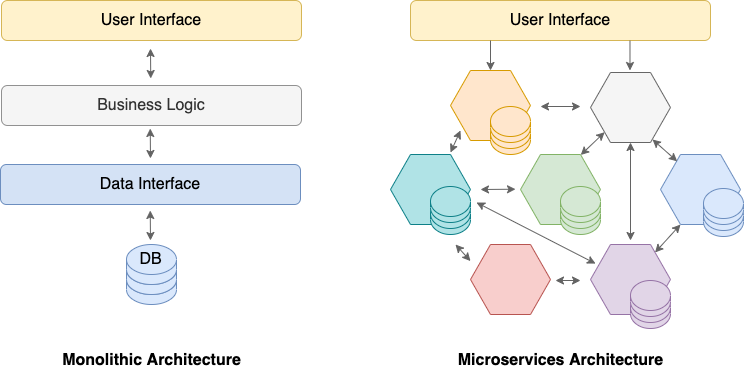
\includegraphics[width=0.9\textwidth]{myImages/monovsmicro.png}
    \caption{Monolithic vs Microservices Architecture}
    \label{fig:monovsmicro}
\end{figure}

Second, the microservice architecture advocates for those services to be small.
It is not easy and in some cases inaccurate (e.g, in terms of LOC) to give an estimate of the magnitude of a service, however, a rule of thumb to keep in mind is, microservices should be small enough and not smaller \cite{newman}.
Each service should focus on one business functionality and do it well.
\\
Third, and the last major aspect that defines the microservice architecture is autonomy.
Each service in the microservice architecture is a separate entity, even to the degree that they are mostly designed, developed and deployed by separate teams.
Each team has staff that can together carry out full range of skills required for development, such as database, UX and project management.
\\
At this point, in order to summarize the mentioned major aspects of the microservice architecture and make the architecture more concrete by adding a bit more detail about the implementation, it is a good opportunity to take a look at the definition of the microservice architecture given by an influential software engineer in the field.
According to Fowler, the microservice architecture is, "in short, an approach to developing a single application as a suite of small services, each running in its own process and communicating with lightweight mechanisms, often an HTTP resource API.
These services are built around business capabilities and independently deployable by fully automated deployment machinery.
There is a bare minimum of centralized management of these services, which may be written in different programming languages and use different data storage technologies."\cite{microdef}.
In the next section, each characteristic of the microservice architecture is explained in more detail.

\subsection{General Characteristics}
\label{subsec:chars}

\begin{itemize}
    \item Each microservice is developed by a small, cross-functional team.
    The team decides which programming language(s) and technology stack to choose to implement the microservice, and has their own CI/CD tools for testing, release and deployment.
    Each microservice is considered not just a project, but a product, and the development teams are responsible also for the deployment and productions processes of their microservice, in the Amazon's notion of "you build it, you run it"\footnote{\href{https://www.infoq.com/news/2015/12/microservices-amazon/}{https://www.infoq.com/news/2015/12/microservices-amazon/}}.
    
    \item Each microservice is a light-weight component that is independently deployable. 
    In case of a change in a particular library, systems that have multiple libraries in a single process like a monolithic architecture has to redeploy entire application. 
    Instead, in a same scenario, having multiple services facilitates redeploying only the changed service. Moreover, this kind of ease in deployment enables the system to be more fault-tolerant and scalable in a more dynamic way, scaling only the desired services, as illustrated Figure~\ref{fig:scalability}, which is adapted from a figure in Fowler's blog\footnote{\href{https://martinfowler.com/articles/microservices.html}{https://martinfowler.com/articles/microservices.html}}.
    
    \begin{figure}[H]
    \centering
    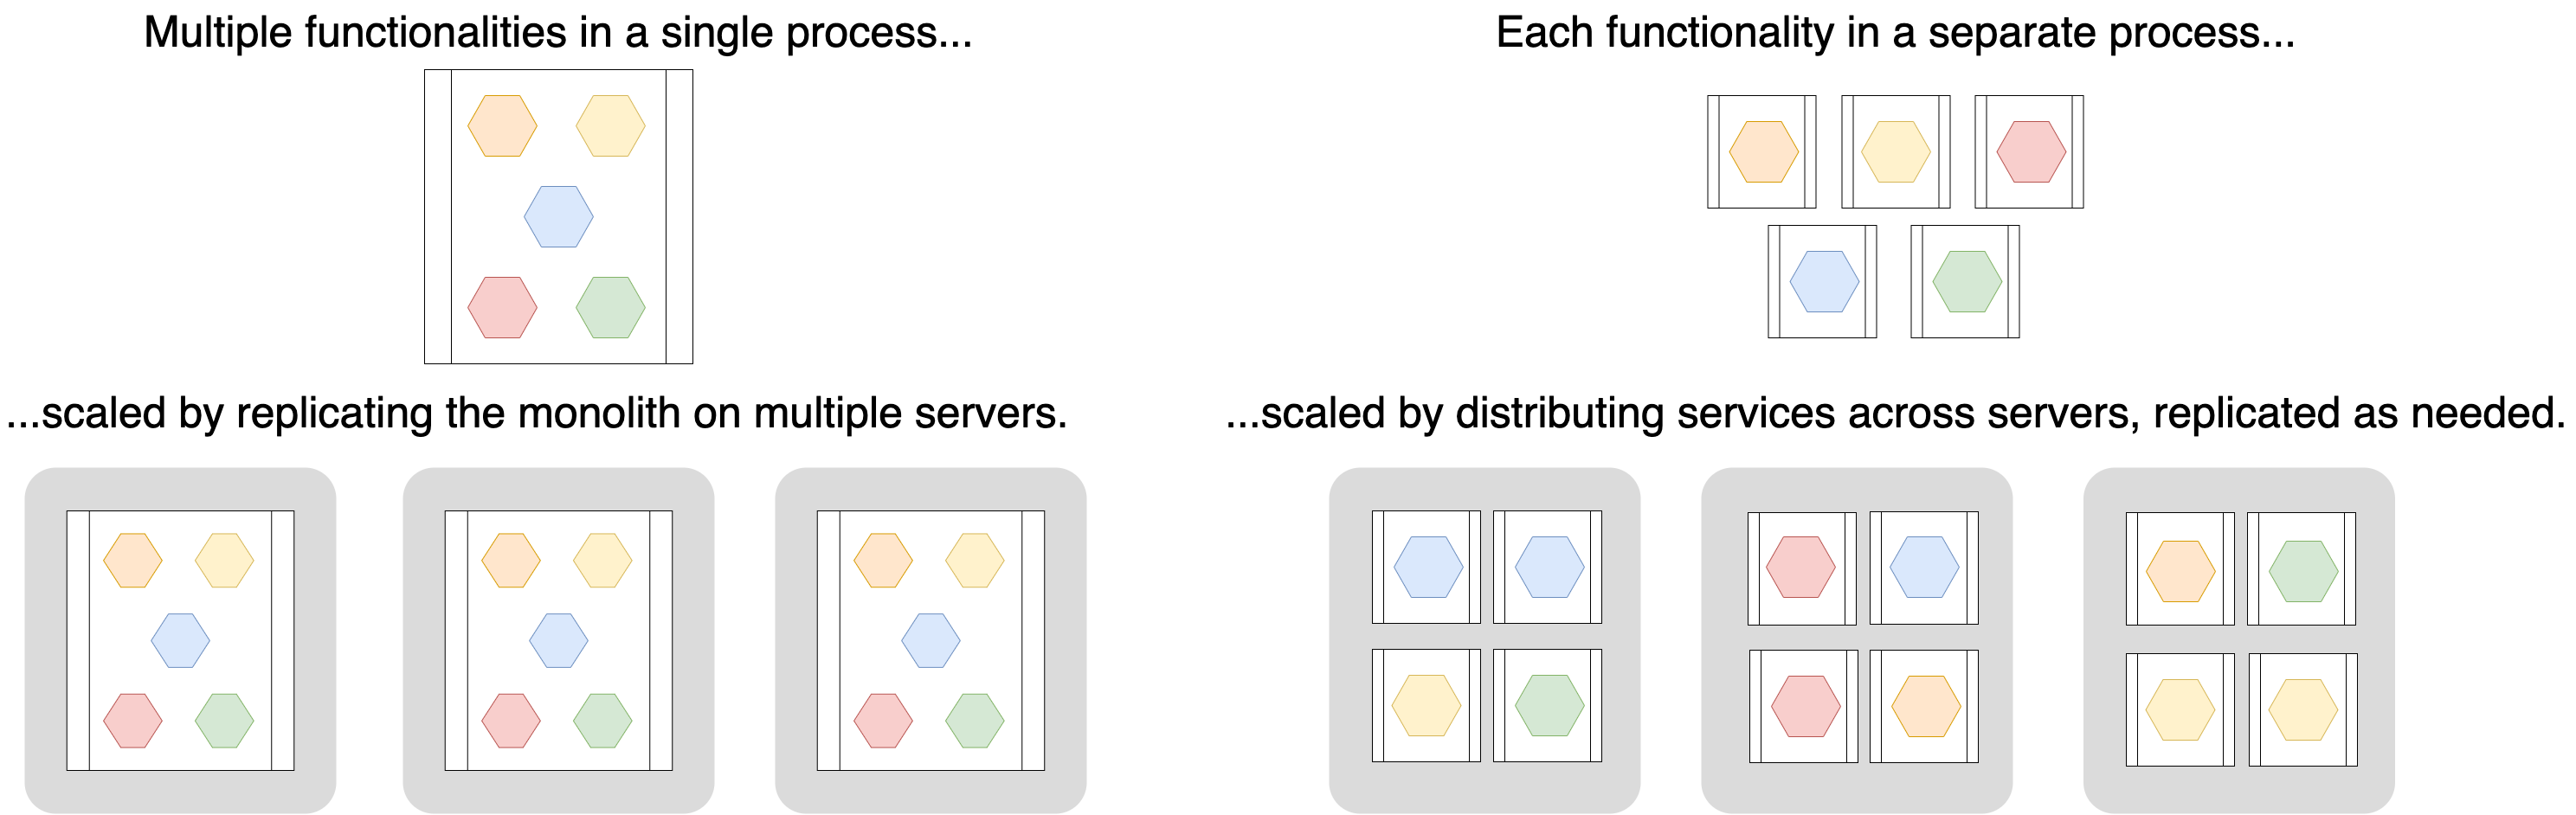
\includegraphics[width=0.90\textwidth]{myImages/scalability.png}
    \caption{Scalability in Monolithic vs Microservice Architectures}
    \label{fig:scalability}
    \end{figure}

    \item Microservices communicate with each other by means of network calls, using well-defined APIs, and simple protocols like REST over HTTP. While some other architectures incorporate smart (and heavy-weight) messaging mechanisms, such as Enterprise Service Buses (ESB) that can do routing, transformation, choreography and some business logic, the microservices architecture opt for simple communication infrastructure that can do basic routing of messages. In short, they have smart endpoints and dumb pipes.
    
    \item Each microservice is a loosely-coupled business unit, that is responsible for a single part of the capabilities of the system.
    Each model of a microservice is designed using the concept of bounded context, which is part of domain driven design technique \cite{boundedcontext}. Conceptual model of the real world entities are decentralized, meaning that the representation (name) and modeling (attributes) of same real world entities might be distinct in microservices that deal with a particular business domain. Figure~\ref{fig:context} illustrates an example bounded context design and highlights the representation of the same entities with different attributes belonging to different business aspect of the system.
    
    \begin{figure}[H]
    \centering
    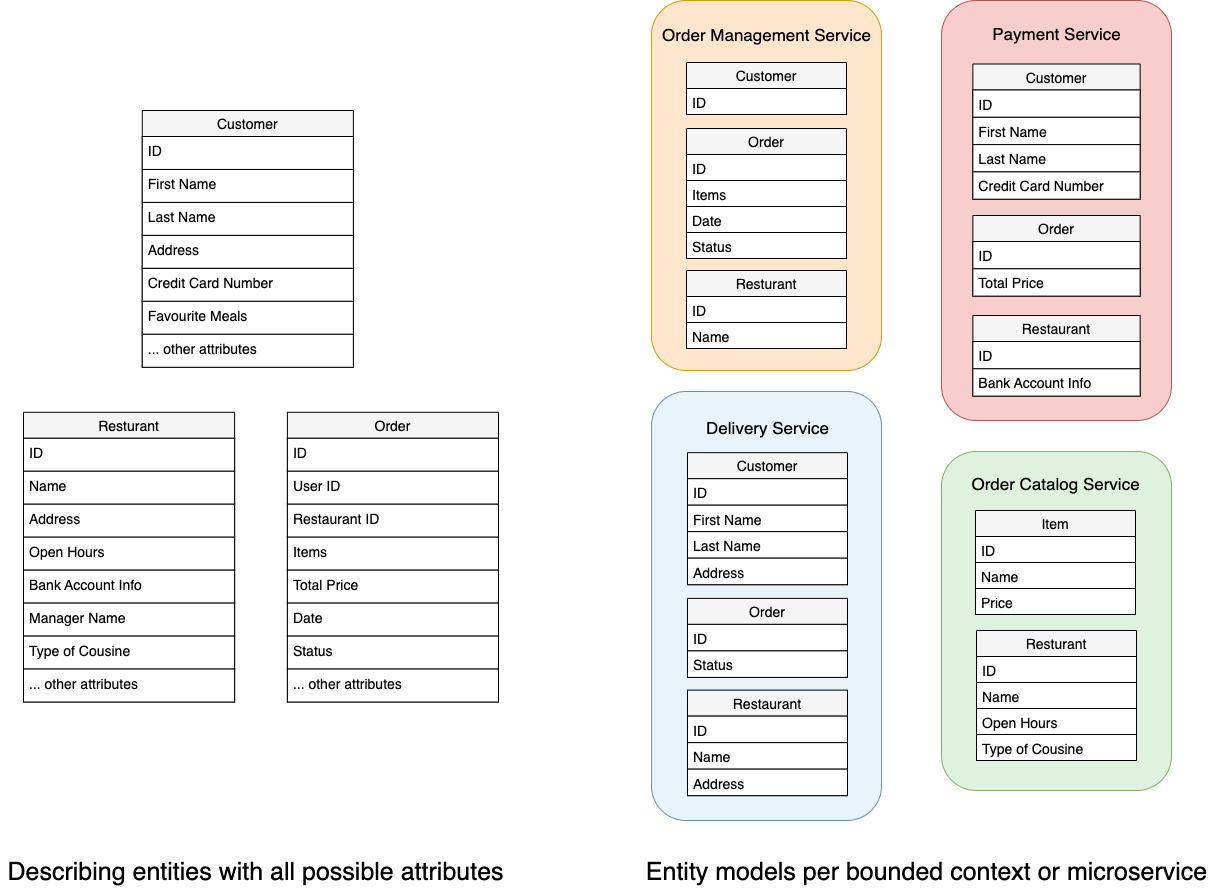
\includegraphics[width=0.93\textwidth]{myImages/context.png}
    \caption{Decomposition methods using traditional vs. bounded context models}
    \label{fig:context}
    \end{figure}

    \item Just like the decentralized modeling, the persistence layer of the whole application is decentralized, in other words, each microservice and associated team is responsible for managing their own data. The team decides on which kind of database (SQL, NoSQL, graph, columnar, etc) they make use of, taking into consideration their own models and needs.

\end{itemize}

\subsection{Differences from Service Oriented Architecture}
\label{subsec:diff}

The profound idea of microservice architecture, which proposes splitting a system into loosely-coupled, reusable, specialized components is not new.
In the late 90's, Service Oriented Architecture (SOA) emerged as an enterprise-wide approach to software development of components that takes advantage of reusable software components, or services.
Similar to microservice architecture, each service is designed to execute business functions.
\\
Although the two architectures look quite identical at the first glance, they take different stands on the solutions of common problems in software architecture and therefore there are substantial differences between the two.
Listing the distinctions under three categories will help explain the difference.

\begin{itemize}
    \item Scope: SOA in general relates to enterprise-wide service exposure, while the microservice architecture has an application scope.
    The services are designed using common standards across development teams, aiming at re-usability and sharing of components, resources and data in SOA.
    On the other hand, microservices architecture embraces more relaxed governance approach, giving development teams more freedom of choice.
    Foregoing potential re-usability of code and data, microservices architecture prefers de-coupling of teams and services.
    
    \item Granularity: Having "re-usability across enterprise-wide system" in mind results in services that are fewer in number and larger in size in SOA.
    Each service typically handles more business functionalities compared to each microservice.
    As for the persistence, SOA has a single data storage layer which is shared by all services, while each microservice has its own persistence mechanism, if needed for its specific business functionality.
    Although this results in data duplication in microservices architecture, it enables each microservice to be an independent business unit in general\footnote{\href{https://www.guru99.com/microservices-vs-soa.html}{https://www.guru99.com/microservices-vs-soa.html}}.
    Moreover, with respect to fine-grained microservices, coarse-grained services in SOA causes time-consuming deployment and less scalability.
    
    \item Communication: SOA makes use of ESB concept, which can handle, in addition to the communication between services using multiple protocols (RESTful API, SOAP, AMQP, MSMQ), management and configuration of services and even some business logic if needed \cite{soa_comm}.
    Having multiple capabilities like these can solve difficult integration problems in large scale systems, however, can possess the danger of single point of failure.
    In addition, the services across the enterprise frequently make synchronous calls, which can lead to latency issues and impact performance.
    To keep things simple, within an application scope, the microservices architecture prefers less elaborate and straightforward  messaging protocols such as HTTP, REST and Apache Thrift\footnote{\href{https://thrift.apache.org}{https://thrift.apache.org}}.
    To provide communication and data synchronization across microservices, asynchronous communication models like event sourcing and pub/sub model are preferred.
\end{itemize}

\section{Design Patterns and Anti-Patterns in Microservices Architecture}
\label{sec:patterns}

Since its introduction by Netflix and discussions at workshops and software architecture conferences, the microservices architecture has gained quite a lot of popularity.
As the architecture is adopted more and more as time goes, legacy systems have been migrated and new projects have been developed utilizing the microservices architecture.
By sharing the experience after successful projects, similar to the evolution of design patterns in other paradigms, reusable solutions to commonly occurring problems have been identified and consequently design patterns in the microservice architecture showed up.
On the flip side, there has also been sub-optimal solutions during this period, resulting from several factors, some of which might be lack of experience, misunderstanding of the microservice architecture or just old habits from SOA.
In the same manner as design patterns, the anti-patterns of the microservice architecture has been identified by researchers and experienced engineers.
In the next two sections, the design patterns and anti-patterns that exist in microservice architectures are explored.
In doing so, in addition to the resources cited in appropriate places, Microsoft Docs website for cloud patterns \cite{microsoft_docs} and microservice patterns book \cite{richardson_book} have been consulted.
For the anti-patterns, the two studies about microservice anti-patterns \cite{10.1145/3424771.3424812}\cite{9522227} have been utilized, details of which are provided as part of the argumentation related to one of the research questions of this study.

\subsection{Design Patterns}
\label{subsec:designpattern}

\subsubsection{API Gateway}
\label{subsubsec:api_gateway}

API gateway acts as a single point of entry for all clients as well as an edge service for exposing microservices to the outside world as managed APIs.
It sounds like a reverse proxy, but also has additional responsibilities like simple load-balancing, authentication, authorization, failure handling, auditing, protocol translations, and routing. An API Gateway should always be a highly-available and performant component, since it is the entry point to the entire system, as illustrated in Figure~\ref{fig:api_gateway}.

\begin{figure}[H]
    \centering
    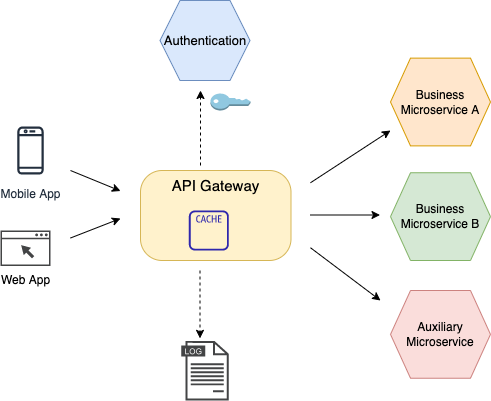
\includegraphics[width=0.6\textwidth]{myImages/APIgw.png}
    \caption{An example diagram of API gateway pattern}
    \label{fig:api_gateway}
\end{figure}

The most common duties of an API gateway include:

\begin{itemize}
    \item Gateway Aggregation: Aggregate multiple client requests (usually HTTP requests) targeting multiple internal microservices into a single client request, reducing chattiness and latency between consumers and services.
    
    \item Gateway Offloading: Enable individual microservices to offload their shared service functionality to the API gateway level.
    Such cross-cutting functionalities include authentication, authorization, service discovery, fault tolerance mechanisms, QoS, load balancing, logging, analytics etc.
    
    \item Gateway Routing (layer 7 routing, usually HTTP requests): Route requests to the endpoints of internal microservices using a single endpoint, so that consumers don’t need to manage many separate endpoints.
\end{itemize}

Developers can choose from implementing their own API gateway, using an existing API gateway solution such as Kong\footnote{\href{https://konghq.com}{https://konghq.com}} or Express-Gateway\footnote{\href{https://www.express-gateway.io}{https://www.express-gateway.io}}, or in case of cloud deployment, choose from products such as Google Cloud Platfrom (GCP) API Gateway\footnote{\href{https://cloud.google.com/api-gateway}{https://cloud.google.com/api-gateway}}, Amazon Web Services (AWS) API Gateway\footnote{\href{https://aws.amazon.com/api-gateway}{https://aws.amazon.com/api-gateway}} or Azure Application Gateway\footnote{\href{https://docs.microsoft.com/en-us/azure/application-gateway/overview}{https://docs.microsoft.com/en-us/azure/application-gateway/overview}}.

\subsubsection{Service Mesh with Sidecar}
\label{subsubsec:service_mesh}

A service mesh is a configurable, low-latency infrastructure layer that is designed to tackle high volume of network-based inter-process communication among  application infrastructure services through APIs.
Service mesh pattern is in general implemented as an array of lightweight network proxies called sidecar, without needing the application to be aware of proxies \cite{li2019service}. The sidecar proxies in each service instance handles inter-process communication, monitoring and many other concerns.
Some aspects provided by this helper infrastructure include resiliency (fault tolerance, load balancing), service discovery, routing, observability, security, access control, communication protocol support and alike.
\\
The service mesh pattern is divided into two parts, namely, the control part and the data part, commonly referred as the control plane and the data plane. The control plane generates routing tables and deploy routing configuration to the proxies in the data plane. The actual forwarding of the network traffic is done by the proxies in the data plane, and for this reason, the data plane is also said to be the forwarding plane. Figure~\ref{fig:service_mesh} shows the diagram of an application with service mesh pattern, with the distinction of the control and data planes.

\begin{figure}[H]
    \centering
    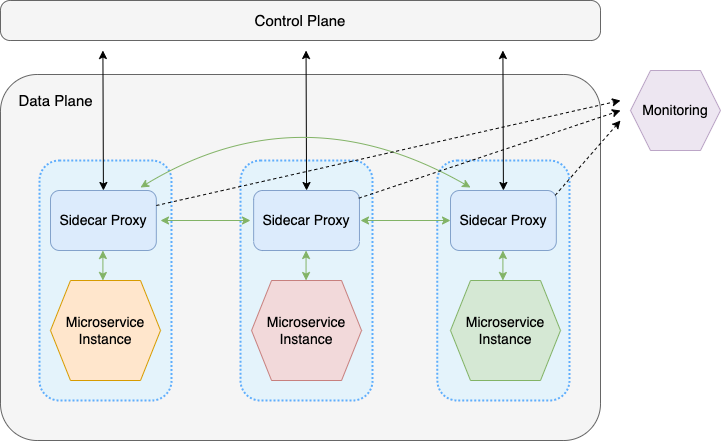
\includegraphics[width=0.75\textwidth]{myImages/mesh.png}
    \caption{An application architecture utilizing service mesh with sidecar proxy}
    \label{fig:service_mesh}
\end{figure}

Some of the advantages of making use of a service mesh are:

\begin{itemize}
    \item Logic Decoupling: Decoupling of network communications from microservice business logic code allows developers to focus on the business capabilities.
    
    \item Routing: Primitive routing capabilities, but no routing logic related to the business functionality of the service.
    
    \item Resiliency for inter-service communications: Circuit-breaking, retries and timeouts, fault injection, fault handling, load balancing and fail-over. 
    
    \item Service Discovery: Discovery of service endpoints through a dedicated service registry.
    
    \item Observability: Metrics, monitoring, distributed logging, distributed tracing.
    
    \item Security: Transport level security (TLS) and key management.
    
    \item Access Control: Simple blacklist and whitelist based access control.
    
    \item Deployment: Native support for containers, Docker\footnote{\href{https://www.docker.com}{https://www.docker.com}} and Kubernetes\footnote{\href{https://kubernetes.io}{https://kubernetes.io}}. 
    \item Support for inter-service communication protocols: HTTP1.x, HTTP2, gRPC\footnote{\href{https://grpc.io}{https://grpc.io}}.
\end{itemize}

Implementations of the service mesh pattern include products such as Istio\footnote{\href{https://istio.io}{https://istio.io}}, Linkerd\footnote{\href{https://linkerd.io}{https://linkerd.io}} and Consul\footnote{\href{https://www.consul.io}{https://www.consul.io}}.

\subsubsection{Service Registry and Discovery}
\label{subsubsec:srd}

In order for services to communicate, they expose a remote API at a particular location, specified by host and port number.
However, the number of service instances and locations change dynamically.
Scaling of services are done thanks to virtualization/containerization technologies and virtual machines and containers are usually assigned dynamic IP addresses.
For a service client to get a service, it needs to know the location of that particular service and this is done through service registry and discovery pattern.
When making a request, the client (of a service, it can be API gateway or another service) consults directly or indirectly to a service registry that keeps the up-to-date addresses of all service instances.
The clients of the service registry need to know the location(s) of the service registry instances, hence service registry instances must be deployed on fixed and well known IP addresses.
Although clients should cache data provided by the service registry, if the service registry fails that data will eventually become out of date. 
Consequently, the service registry must be highly available.

\begin{itemize}
    \item Service Registry: Service instances register themselves or a third party registers the service.
    A service registry might invoke a service instance’s health check API to verify that it is able to handle requests.
    Systems that provide service registry include middlewares such as Netflix Eureka\footnote{\href{https://github.com/Netflix/eureka}{https://github.com/Netflix/eureka}}, Apache Curator\footnote{\href{https://curator.apache.org}{https://curator.apache.org}} with centralized configuration service Apache Zookeeper\footnote{\href{https://zookeeper.apache.org}{https://zookeeper.apache.org}}; and service meshes such as Consul and distributed key-value stores such as Etcd\footnote{\href{https://etcd.io}{https://etcd.io}}.
    Some other systems such as Kubernetes and AWS Elastic Load Balancer (ELB)\footnote{\href{https://aws.amazon.com/elasticloadbalancing}{https://aws.amazon.com/elasticloadbalancing}} have implicit service registry.
    
    \item Client-side Service Discovery: Query (of service registry) logic is built into the client.
    In other words, it is the client who has to talk to the service registry to learn the host address and port number to make the final request to the service it is interested in.
    Spring Cloud framework\footnote{\href{https://spring.io/projects/spring-cloud}{https://spring.io/projects/spring-cloud}} provides client-side service discovery, which is implemented by Netflix Open Source Software components: service registry Eureka and HTTP client Ribbon\footnote{\href{https://github.com/Netflix/ribbon}{https://github.com/Netflix/ribbon}} that queries Eureka registry.
    
    \item Server-side Service Discovery: The client makes the request via a router that runs on a well known location.
    The router queries the service registry, which might as well be built into the router, and forwards the request to an available service instance.
    Hence, server-side service discovery results in simpler client code, since it is the router who has to implement the actual service query logic.
    As an example, AWS ELB acts as a router that load balances both external and internal traffic and also acts as a service registry for AWS EC2 instances.
    Some clustering solutions such as Kubernetes run a proxy (“service” in Kubernetes terminology) on each host, which functions as a server-side discovery router.
    In order to access a service, a client connects to its local proxy service using the port assigned to that service.
    The proxy then forwards the request to a service instance or to controller such as Ingress-nginx\footnote{\href{https://github.com/kubernetes/ingress-nginx}{https://github.com/kubernetes/ingress-nginx}} running in the cluster.

\end{itemize}

\subsubsection{Backends For Frontends}
\label{subsubsec:bff}

Instead of using one common backend service for multiple clients, there are separate deployments of the same service with different configurations or implementations that can meet different UI requirements of different clients.
Each microservice that implements backends for frontends pattern provides an API, tailored specifically for one kind of client.
Because each backend is specific to one kind of client, it can be optimized for the interface the client uses.
As an example, while a microservice returns the detailed result of a query for the web application to use, another microservice with the same business capability, implemented with slightly different logic or configuration can return a concise version of the result to a mobile client.
As a result, each interface team has autonomy to control their own backend and does not need to rely on a centralized backend development team.

\subsubsection{Asynchronous Messaging}
\label{subsubsec:async_msg}

The distributed nature of microservices requires messaging mechanisms, ideally in a loosely-coupled manner.
The synchronous messaging results in tight run-time coupling, that is, both the client and the service need to be available during the whole messaging period.
To solve these issues and improve scalability, asynchronous messaging mechanisms are widely used in microservices architecture.
Solutions typically include light-weight event buses and message brokers.
Although an extra layer adds complexity, event buses and message brokers decrease run-time coupling by buffering messages, in other words, allowing the recipient to process messages when it becomes available.
Moreover, topics and content filtering can be used to create subsets of messages, delivered only to the interested parties.
With the help of built-in mechanisms of message brokers, different asynchronous messaging styles such as request/response, notification and publish/subscribe can be achieved.
Figure~\ref{fig:rabbitmq} illustrates an example diagram that includes RabbitMQ\footnote{\href{https://www.rabbitmq.com}{https://www.rabbitmq.com}} as a message broker, providing the publish/subscribe messaging manner.

\begin{figure}[H]
    \centering
    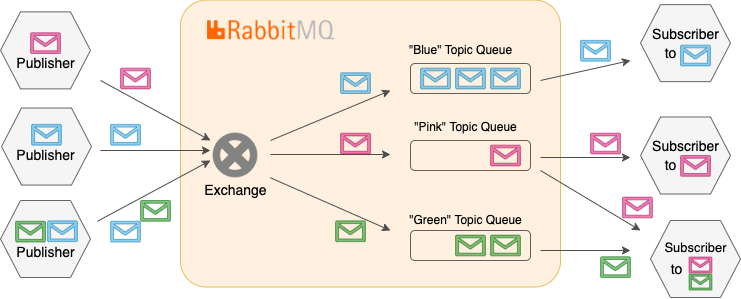
\includegraphics[width=0.9\textwidth]{myImages/asynch_messaging.png}
    \caption{RabbitMQ message broker with pub/sub mechanism}
    \label{fig:rabbitmq}
\end{figure}

Implementations of message brokers include RabbitMQ and Apache Kafka\footnote{\href{https://kafka.apache.org}{https://kafka.apache.org}}.
The in-memory database Redis\footnote{\href{https://redis.io}{https://redis.io}} can also be used as a message broker.
In addition, cloud providers offers message brokers and event buses with different capabilities, such as AWS Simple Notification Service (SNS)\footnote{\href{https://docs.aws.amazon.com/sns/latest/dg/welcome.html}{https://docs.aws.amazon.com/sns/latest/dg/welcome.html}}, AWS Simple Queuing Service (SQS)\footnote{\href{https://docs.aws.amazon.com/sqs/}{https://docs.aws.amazon.com/sqs/}}, AWS Eventbridge\footnote{\href{https://aws.amazon.com/eventbridge}{https://aws.amazon.com/eventbridge}}, Azure Service Bus\footnote{\href{https://docs.microsoft.com/en-us/azure/service-bus-messaging/service-bus-messaging-overview}{https://docs.microsoft.com/en-us/azure/service-bus-messaging/service-bus-messaging-overview}} and GCP Pub/Sub\footnote{\href{https://cloud.google.com/pubsub/docs/overview}{https://cloud.google.com/pubsub/docs/overview}}.

\subsubsection{Database per Service}
\label{subsubsec:dps}

For the sake of loose-coupled services, each service’s persistent data is private to that service and accessible only via its API.
Even though keeping private tables or schema per service facilitates private data, having separate database instances per service also enables the deployment and scaling of services and allows the teams to be more independent.
By this means, each service can use the type of database that is best suited to its needs.
For example, an archiving service that provides fast text searches could use ElasticSearch\footnote{\href{https://www.elastic.co}{https://www.elastic.co}}, while
another service that models social interactions using graphs could use graph database Neo4j\footnote{\href{https://neo4j.com}{https://neo4j.com}}.
Although having a separate database server per service is aligned with loose coupling idea, it increases complexity in terms of implementation of transactions that span multiple services, since not all No-SQL databases support atomic commits among distributed database instances, which are in general implemented using atomic transaction algorithms (two-phase or three-phase commit) in ACID-compliant relational databases.

\subsubsection{Saga}
\label{subsubsec:saga}

In order to solve the issue of implementing business transactions across multiple services, each multi-service transaction is implemented as a sequence of local transactions, which is called a saga.
If a local transaction fails because it violates a business rule then the saga executes a series of compensating transactions that undo the changes that were made by the preceding local transactions.
The two ways of implementing a saga pattern are:

\begin{itemize}
    \item Choreography-based Saga: A transaction is first targeted to a particular service (“order” service receives a POST request to "/orders").
    The service completes local transaction with its own database and emits an event to the event bus or a particular event channel (“order created” event in “order events” or a common channel).
    The service that subscribed to that kind of event sees the emitted event and does its own logic and local transaction to its own database and emits another event for any service that listens for that kind of event.
    If all steps are successful, the last service will let the first service know by emitting an event.
    Otherwise, if a failure occurs in a step, the service that could not get its job done (in terms of logic or infrastructure) fires a failure event for the previous step, so the services that have worked before this step can sequentially perform rollbacks.
    
    \item Orchestration-based Saga: In this approach, unlike the above method, there is an orchestrator that manages the entire transaction.
    When a transaction order that is related to multiple services comes to the service, the service sends a command to the orchestrator.
    The orchestrator starts calling services to be called directly or indirectly and after a successful response, it calls the next one. Upon an answer that tells about a failure, the orchestrator then starts sending rollback messages to the previous services.
    With respect to the choreography approach, this method brings about scalability and single point of failure issues.
\end{itemize}

In addition, in some systems where saga or event sourcing patterns are used, transactional outbox method solves the issue of atomicity between changing the state and sending of messages, if there are requirements that are not met with eventual consistency and require atomicity.
A business microservice that uses a relational database inserts messages/events into an outbox table in the database as part of the local business logic transaction, with an additional boolean attribute that means "unpublished" for newly created messages, and "published" for messages that are acknowledged by message relay service.
A separate message relay service either polls the outbox table or reads the transaction log of business services, to get the "unpublished" messages.
Then, the message relay service sends those "unpublished" messages to a message broker that delivers messages to interested parties.
The message relay service then waits for acknowledgement from message broker, and upon an acknowledgement, changes the status of successfully sent "unpublished" messages to "published" in the outbox table of the business microservice.
In short, by storing messaging as part of business transaction in the DBMS and using a buffer service between business microservices and message broker, the atomicity between database transactions and messages can be achieved.

\subsubsection{API Composition}
\label{subsubsec:api_comp}

A simple way to implement queries that spans multiple services is API composition pattern.
API composer service can take the query, then starts querying individual services that are related to the main query, join the responses and format the main query result to the client.
However, some queries would result in inefficient, in-memory joins of large datasets.

\subsubsection{Command Query Responsibility Segregation (CQRS)}
\label{subsubsec:cqrs}

Another way to respond to a query that covers numerous services is Command Query Segregation Pattern.
A service is wrapped around a view database that is a read-only replica that fulfils the query responsibility of the application.
The service keeps the database up-to-date by subscribing to domain events, published by the service that owns the data.
As the name suggests, separate services are responsible for the query (read) and command (write and any other logic) parts of the application.
Although it comes with potential complexity, code duplication and eventually consistent view nature, it supports multiple de-normalized views that are scalable and performant in terms of command and query throughput.

\subsubsection{Event Sourcing}
\label{subsubsec:event_sourcing}

A microservice typically needs to update its data and send or publish messages that conveys some information about the transaction or related business action.
For example, a service that participates in a saga needs to atomically update the database and sends messages or events.
If the database transaction is executed successfully, resulting messages must be sent and later, if the entity in the database rolls back to its previous state or changed again into a new state, related appropriate messages must be send to interested microservices.
In addition, the  ordering of messages must be preserved across multiple service instances that update the same entity.
\\
A good solution to this problem is to use event sourcing pattern.
Event sourcing persists the state of a business entity such as Order or a Customer as a sequence of state-changing events.
Whenever the state of a business entity changes, a new event is fired from the respective microservice, and stored in a database named as the event store, which can be an ACID-compliant database, a time-series database or a database server specifically implemented for event sourcing pattern, such as EventStore\footnote{\href{https://www.eventstore.com}{https://www.eventstore.com}}.
The most recent state of the application data is constructed by processing the events and storing the data in a materialised view that handles read-only queries.
Embracing the eventual consistency paradigm, the materialised view can be updated according to the constraints of the domain of the application, by finding the most recent snapshot of the application data and processing the persisted events that have occurred since that snapshot. Figure~\ref{fig:event_sourcing} illustrates the flow and storage of the events in a possible software version tracking application that makes use of event sourcing pattern, where event store is benefited especially for temporal queries that show the state of the software in a particular point in time.

\begin{figure}[H]
\centering
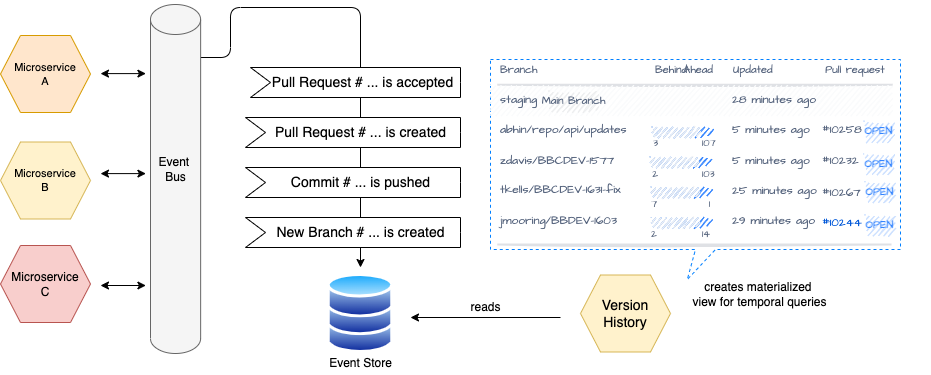
\includegraphics[width=1\textwidth]{myImages/event_store.png}
\caption{A possible use of event sourcing pattern for a software version tracking application}
\label{fig:event_sourcing}
\end{figure}

Moreover, event sourcing pattern makes it possible to implement temporal queries that determine the state of an entity at any point in time.
Append-only storage mechanism enables to see the actions taken related to a particular set of data, as well as assisting in testing and debugging \cite{event_sourcing_docs}.

\subsubsection{Service Instance per Virtual Machine}
\label{subsubsec:per_vm}

The microservices architecture promotes some ideas also for the deployment stage of the software lifecycle and these ideas are, as expected, built around loose-coupling paradigm.
The first of these patterns regarding the deployment process is service instance per virtual machine (VM) pattern.
Basically, in this method, each microservice is packaged as a VM image and deployed as an application running in its own VM, possibly with other VMs running on an hypervisor-based machine which is managed by Infrastructure-as-a-Service (IaaS) provider, such as AWS Elastic Compute Cloud (EC2) \footnote{\href{https://aws.amazon.com/ec2/}{https://aws.amazon.com/ec2/}}, Google Compute Engine\footnote{\href{https://cloud.google.com/compute}{https://cloud.google.com/compute}} and Digital Ocean\footnote{\href{https://www.digitalocean.com}{https://www.digitalocean.com}}.
Packaging of a service as a VM image results in ease of scaling of services, which can also be automatically done by the IaaS provider based on the load.
Moreover, the details of the implementation of the service can be encapsulated in a VM image, therefore the dependence of the service technology over the physical host can be reduced.
With regard to the drawbacks, it is time-consuming for developers to create VM images and configure infrastructure components such as load balancers and firewalls.

\subsubsection{Service Instance per Container}
\label{subsubsec:per_container}

Another microservice pattern regarding the deployment aspect is service instance per container pattern.
Similar to packaging each service as a VM image, this pattern proposes packaging each service as a container image, in most cases, as a Docker image.
According to the official docs, Docker is an open platform for developing, shipping, and running applications, and provides the ability to package and run an application in a loosely isolated environment called a container \cite{docker_def}.
Docker containers provide many of the same advantages as VM images, however, due to the underlying virtualization method, Docker containers are much more lightweight with respect to VMs \cite{eder2016hypervisor}.
Rather than using a separate operating system, containers share a operating system, resulting in a significantly smaller size of each deployment.
Underneath, Docker make use of "linux kernel namespaces" and "control groups" to isolate resources of a single virtual or physical host (resources of a single operating system in both cases) and allows Docker containers and services inside to consume resources of the host.
Being a more "micro" approach, containers make it easier for developers to package and share an application through Docker Hub\footnote{\href{https://hub.docker.com}{https://hub.docker.com}} and deploy a service as a container image, which is built with specifications taken from a "Dockerfile", to a private cloud or a Container-as-a-Service (CaaS) provider, such as Google Cloud Run\footnote{\href{https://cloud.google.com/run}{https://cloud.google.com/run}} or AWS Fargate\footnote{\href{https://aws.amazon.com/fargate}{https://aws.amazon.com/fargate}}.
Moreover, the overall resiliency of the application can be improved since it takes less time and effort to run a container with respect to a service with its own operating system.
For the sake of a clear understanding of the two virtualization methods mentioned and how they differ from traditional deployment methods, the evolution of concepts are illustrated in Figure~\ref{fig:hypervisor_vs_container}. As a side note, it is interesting to see the same evolution towards fine-granularity, seen in application architecture from monoliths and SOA to microservices, also in software deployment approaches.

\begin{figure}[H]
\centering
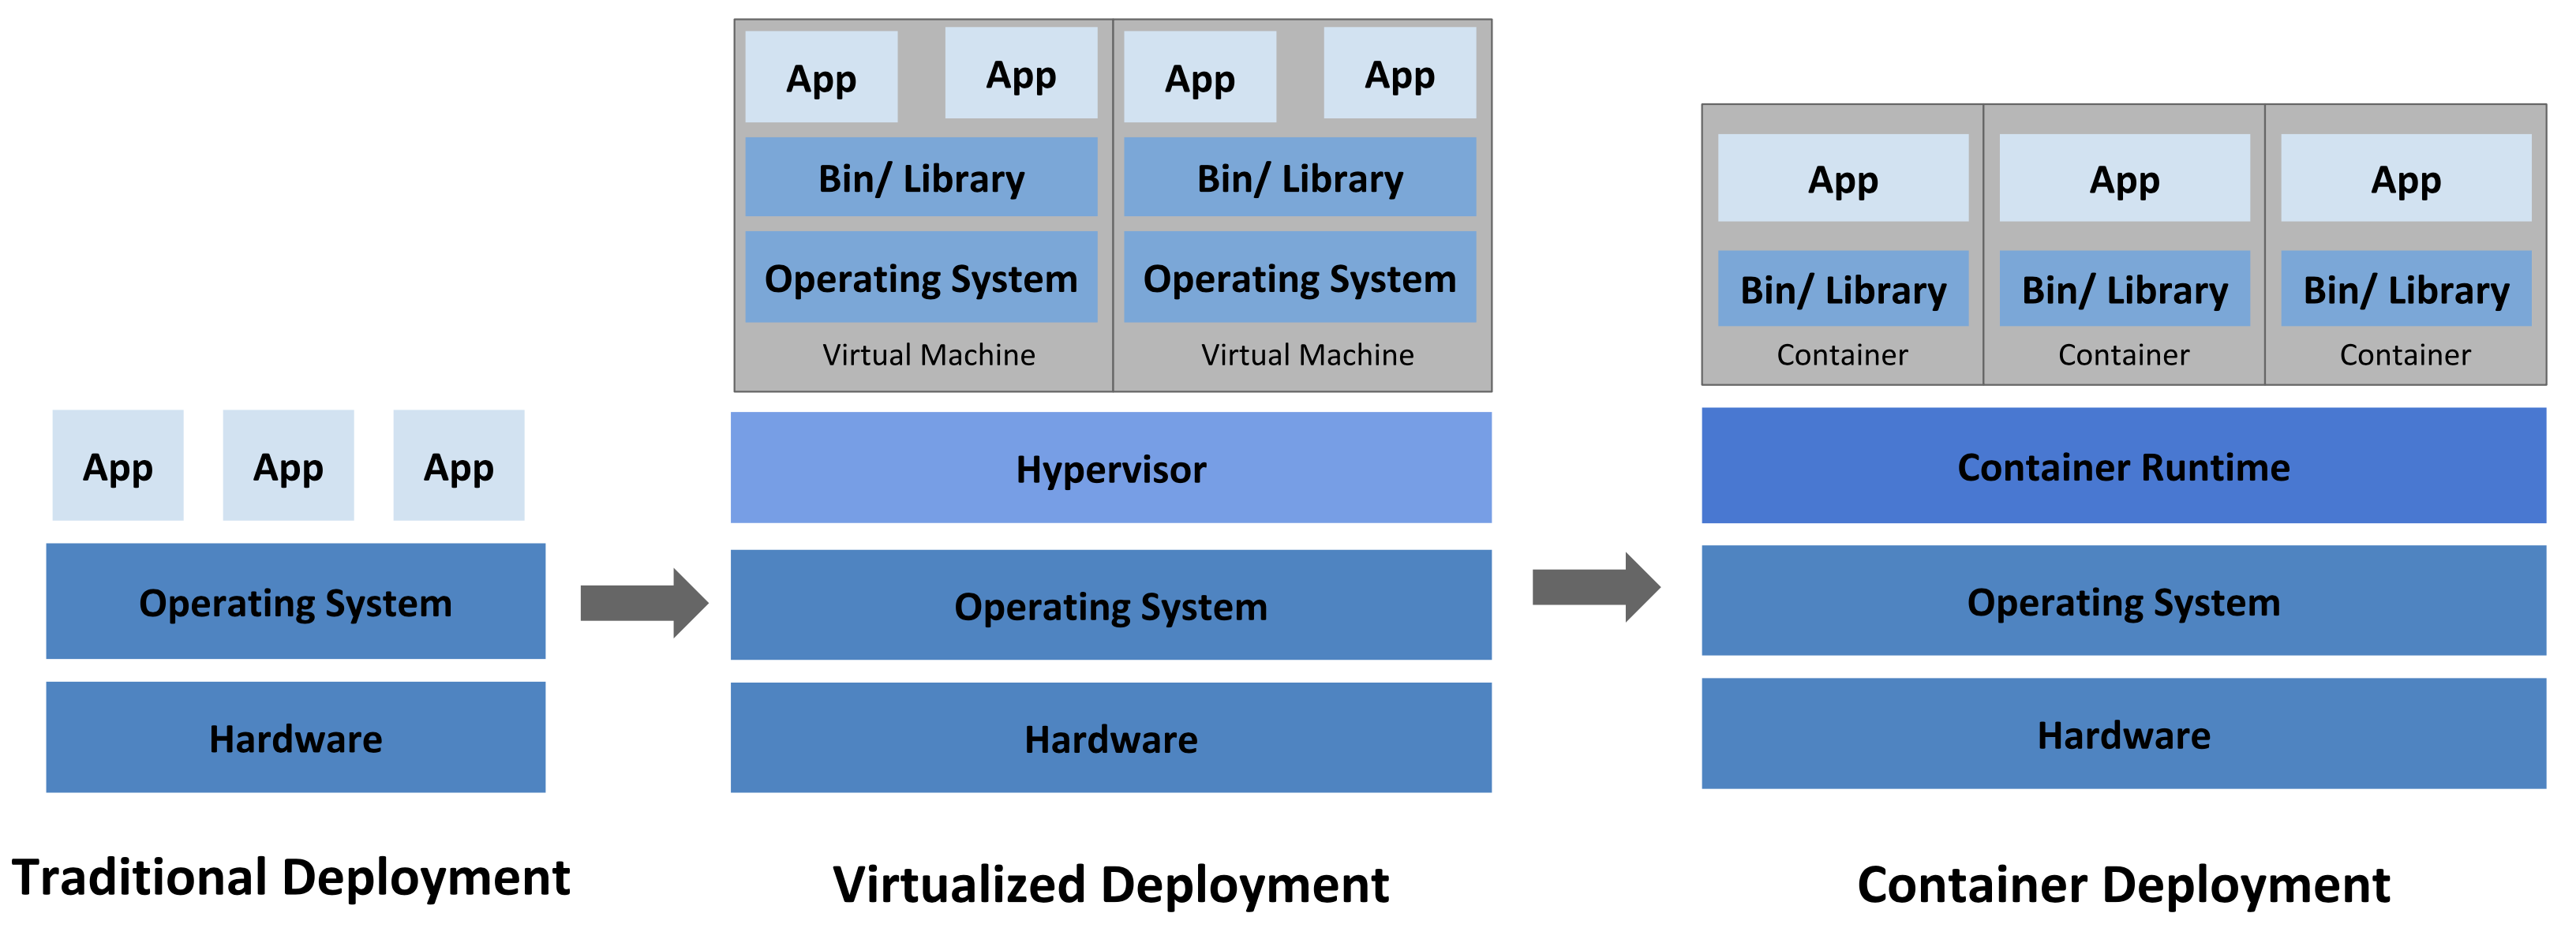
\includegraphics[width=0.95\textwidth]{myImages/kubernetes_evo.png}
\caption{Comparison and evolution of traditional, hypervisor-based and container-based deployment, by Kubernetes Documentation under CC-BY-4.0 license}
\label{fig:hypervisor_vs_container}
\end{figure}

Microservice applications consist of tens or hundreds of microservices, and considering multiple instances for some services, the total number of service instances can be quite high.
In order for the advantages promised by the microservices architecture, supposing the adoption of container-based deployment, the cluster of containers must be properly instantiated, managed and observed.
To simplify the management of a cluster of containers, there are container orchestration platforms, such as Kubernetes and AWS Elastic Container Service (ECS)\footnote{\href{https://aws.amazon.com/ecs}{https://aws.amazon.com/ecs}}, in addition to a few deprecated tools, such as Docker Swarm and Mesosphere.
Kubernetes was initially developed by Google, open-sourced in 2014 and since then has been the most widely used container orchestration platform, according to a 2019 survey\cite{hackernoon} by Cloud Native Computing Foundation\footnote{\href{https://www.cncf.io}{https://www.cncf.io}}.
At this point, to see how containerization technology and orchestration platforms comes together to realize a microservices application, it is crucial to mention some capabilities of Kubernetes and challenges it tackles.
According to official documentation\cite{kubernetes_docs}, some of the features of Kubernetes are:
\begin{itemize}
    \item Service Discovery and Load Balancing: Kubernetes exposes container via a DNS name or IP address to the cluster, can deploy an "ingress-nginx" component that can act as an API gateway, and can distribute network traffic between service instances if the load is high.
    
    \item Storage orchestration: Allows mounting (attaching, binding) of different storage options such as local storage and public cloud provider, to the containers.
    
    \item Automated rollouts and rollbacks: Enables developers to describe the desired state of the containers at hand and via a feed-back mechanism, tries to realize the desired state into the actual state of the cluster. In other words, "rolls out" changes in a progressive way and if something bad happens, "rolls back" changes to the previous stable state. It can create or remove containers and some kinds of Kubernetes objects such "Pods", "Deployments" and "Services" to carry out the task.
    
    \item Automatic bin packing: When provided with the information of how much CPU and memory a container needs, Kubernetes can figure out how to place containers to a set of nodes so that the resources are best utilized.
    
    \item Self-healing: Restarts containers that failed, and based on user-defined health-check, replaces or kills containers that do not respond. Moreover, it routes traffic to healthy instances until the failed container is ready to handle requests.
    
    \item Secret and Configuration Management: Stores and manages sensitive information such as passwords, OAuth access token and SSH keys. Without having to re-build container images, stores and updates application configuration such as environment variables.
\end{itemize}

In addition to stand-alone Kubernetes platform for on-premise solution, the cloud providers offer Kubernetes-as-a-Service options, such as Google Kubernetes Engine (GKE)\footnote{\href{https://cloud.google.com/kubernetes-engine}{https://cloud.google.com/kubernetes-engine}}, AWS Elastic Kubernetes Service (EKS)\footnote{\href{https://aws.amazon.com/eks/}{https://aws.amazon.com/eks/}} and Azure Kubernetes Service (AKS)\footnote{\href{https://azure.microsoft.com/en-us/services/kubernetes-service/}{https://azure.microsoft.com/en-us/services/kubernetes-service/}}, that enables to run Kubernetes clusters on the cloud, by means of container images and Kubernetes configuration files.
\\
As a consequence of the capabilities explained above, and as also stated by researchers from IBM in a research paper \cite{jaramillo2016leveraging}, it is appropriate to say that Docker has been a disruptive technology which changed the way applications are developed and distributed.
Following the same concepts and ideas as microservices architectural paradigm itself, Docker is quite a good fit for building and deploying microservices.

\subsubsection{Serverless}
\label{subsubsec:serverless}

To deploy a microservice application, the services as source codes can be packaged (e.g., as a ZIP file) and uploaded to the deployment infrastructure, which is an utility operated by a public cloud provider.
The infrastructure hides any concept of servers, resources, virtual machines and containers, it just takes the code and runs it.
Under the hood, it uses virtual machines and containers to isolate the services.
The client (of this service) is charged for each request based on the resources consumed.
This solution is very elastic in terms of scaling, however, it comes with significant constraints in the environment.
As an example, AWS Lambda\footnote{\href{https://aws.amazon.com/lambda}{https://aws.amazon.com/lambda}} limits the maximum time it can take for a microservice to serve a request to be fifteen minutes, making it unsuitable for microservices that need to execute for longer amount of time, such as data-processing batch jobs \cite{aws_lambda}.
Another important constraint in serverless pattern is, the microservices need to be "stateless", in other words, the microservice should not assume the existence of a particular data in its local file storage or memory to serve requests, instead, the state should be stored in persistence services such as AWS Simple Storage Service (S3)\footnote{\href{https://aws.amazon.com/s3/}{https://aws.amazon.com/s3}}.
Constraints such as these allow small microservices to be instantiated quickly, making it suitable for developers to deploy not the entire microservice application but some particular microservices that are not called frequently enough to be deployed to its own host, reducing the insfrastructure costs.
Examples include AWS Lambda, Google Cloud Functions\footnote{\href{https://cloud.google.com/functions}{https://cloud.google.com/functions}}, Azure Functions\footnote{\href{https://docs.microsoft.com/en-us/azure/azure-functions}{https://docs.microsoft.com/en-us/azure/azure-functions}}.

\subsubsection{Health Check API}
\label{subsubsec:health_check_api}

Microservices, like any other software component, can crash or fail to serve the requests even if they still run.
During the times of unavailability, it is critical to notice those services that cannot carry out requests so that the requesting services do not wait unnecessarily, and instead, if there is another healthy instance of the failing service, are routed to those available instances.
Since the scope of a microservice is in general small, the availability status in terms of sufficient disk memory, connection to a database or a cache service or in general any other service it is dependant upon, can be coded or created from features of the framework being used.
As an example, the microservice can have an health check endpoint such as "/api/v1/health", and can respond to GET request with the status of the service described in a simple JSON file, possibly with one of the HTTP status codes such as 200, 204, 500 or 503 which stand for "OK", "No Content", "Internal Server Error" and "Service Unavailable", respectively.
\\
In addition to health check mechanisms as code, the container orchestration platform Kubernetes offers health check methods that can be configured descriptively in Kubernetes configuration files by developers.
Kubernetes offers two kinds of health checking or "probing" options, named as liveness and readiness, and can carry out the health checks in periodic time intervals specified.
The first type, liveness, refers to whether a set of one or more containers, also knows as a "pod", is responsive or not.
In cases of a crash or a deadlock situation, restarting the pod can help make the service available again.
The second type, readiness, is used to decide if the service is ready to serve the requests, i.e., serves request only after loading data or configuration files or checking with services it depends on.
The health check API pattern, as seen from examples, is in fact helpful to detect and manage failures in microservices and hence in the whole system, improving the resiliency of the application.

\subsubsection{Log Aggregator}
\label{subsubsec:log_aggregator}

As mentioned in the previous health check API pattern, from time to time, microservices may fail to serve the request and in some cases, it takes more than simply restarting the service to solve the issue.
Developers might need to take a look in the log files to find the exact cause of the problem.
In a microservice application, however, inspecting log files of a microservice by connecting to its host can be frustrating.
One reason is, there can be multiple instances of a microservice on different hosts, and it would be time-consuming to find the right host, especially if the services are scaled to new hosts automatically.
Another reason might be that, merely finding log files in most cases does not suffice to remove the bug, but trouble-shooting the microservices and comparing the logs from a chain of microservices is needed.
In order to ease the trouble-shooting process, log aggregator pattern can be utilized.
\\
Essentially, what log aggregator pattern proposes is, creating a central service and simply aggregating all log files from other microservices instances. Although this is simple idea, with some additions, the trouble-shooting process and developer experience can be significantly improved.
Through a configuration or log aggregator service, different logging types with various levels of detail can be specified during run-time of microservices.
After creating a structured logging for all microservices with appropriate fields, to some extent, aggregated log files can be searchable.
Furthermore, advanced analyzing tools can be used to have more insights about the whole system.
As an example, ElasticSearch, Logstash and Kibana tools, also known as the "ELK" stack\footnote{\href{https://www.elastic.co/elastic-stack}{https://www.elastic.co/elastic-stack}}, are widely used for this purpose.
From microservices themselves or from a message broker, the logs are sent to data ingestion tool Logstash, and afterwards, ElasticSearch is used to analyze text or JSON data and Kibana is used to visualize the results to make the data more presentable for developers and data analysts.
Another example from a public cloud provider is AWS CloudWatch\footnote{\href{https://aws.amazon.com/cloudwatch}{https://aws.amazon.com/cloudwatch}}.
In addition to above-mentioned capabilities of ELK stack, CloudWatch can be configured to send alerting events or do some operational changes such as auto-scaling, if a particular word or a message occurs among the logs.

\subsubsection{Distributed Tracing}
\label{subsubsec:distributed_tracing}

In a microservice-based application, in contrary to a monolithic application, a request does not get handled by a single software component but rather by multiple microservices needed for that particular request.
From a system-wide point of view, a request, whether it is from an external UI agent or an internal microservice for a background job, results in an execution of a chain of microservices.
Naturally, this type of multi-call mechanism of microservices brings about complexity in terms of application development and performance monitoring.
For example, it would be helpful for developers to see which microservices are being called and which bounded domain contexts are being touched by a specific request.
Another exemplary scenario is that, some microservices might take more time to execute their tasks before calling the next microservice in the chain, so it would be beneficial to acquire how long it takes for microservices to complete their tasks so that the bottleneck of the system can be pinpointed and improved.
For these kind of tasks, distributed tracing pattern can be quite advantageous.
\\
In essence, distributed tracing pattern suggests assigning IDs to each external requests and passing it along with each call down the chain or path of execution, so that the path can be traced.
Each microservice is attached or instrumented with an agent that creates new spans for incoming requests and attaches context information required for identification to outgoing request.
Similar to log aggregator pattern, a central collector service receives trace data from agents, validates and stores data to be queried.
Finally, a query process queries the tracing database and shows the result of the query, possibly as a visualization using nodes, arrows, nested spans and related data.
Figure~\ref{fig:jaeger_trace} illustrates a detailed view of inter-service calls resulted from a GET request to an endpoint in frontend service, created by Jaeger\footnote{\href{https://www.jaegertracing.io}{https://www.jaegertracing.io}}, which is an open-source distributed tracing system.

\begin{figure}[H]
\centering
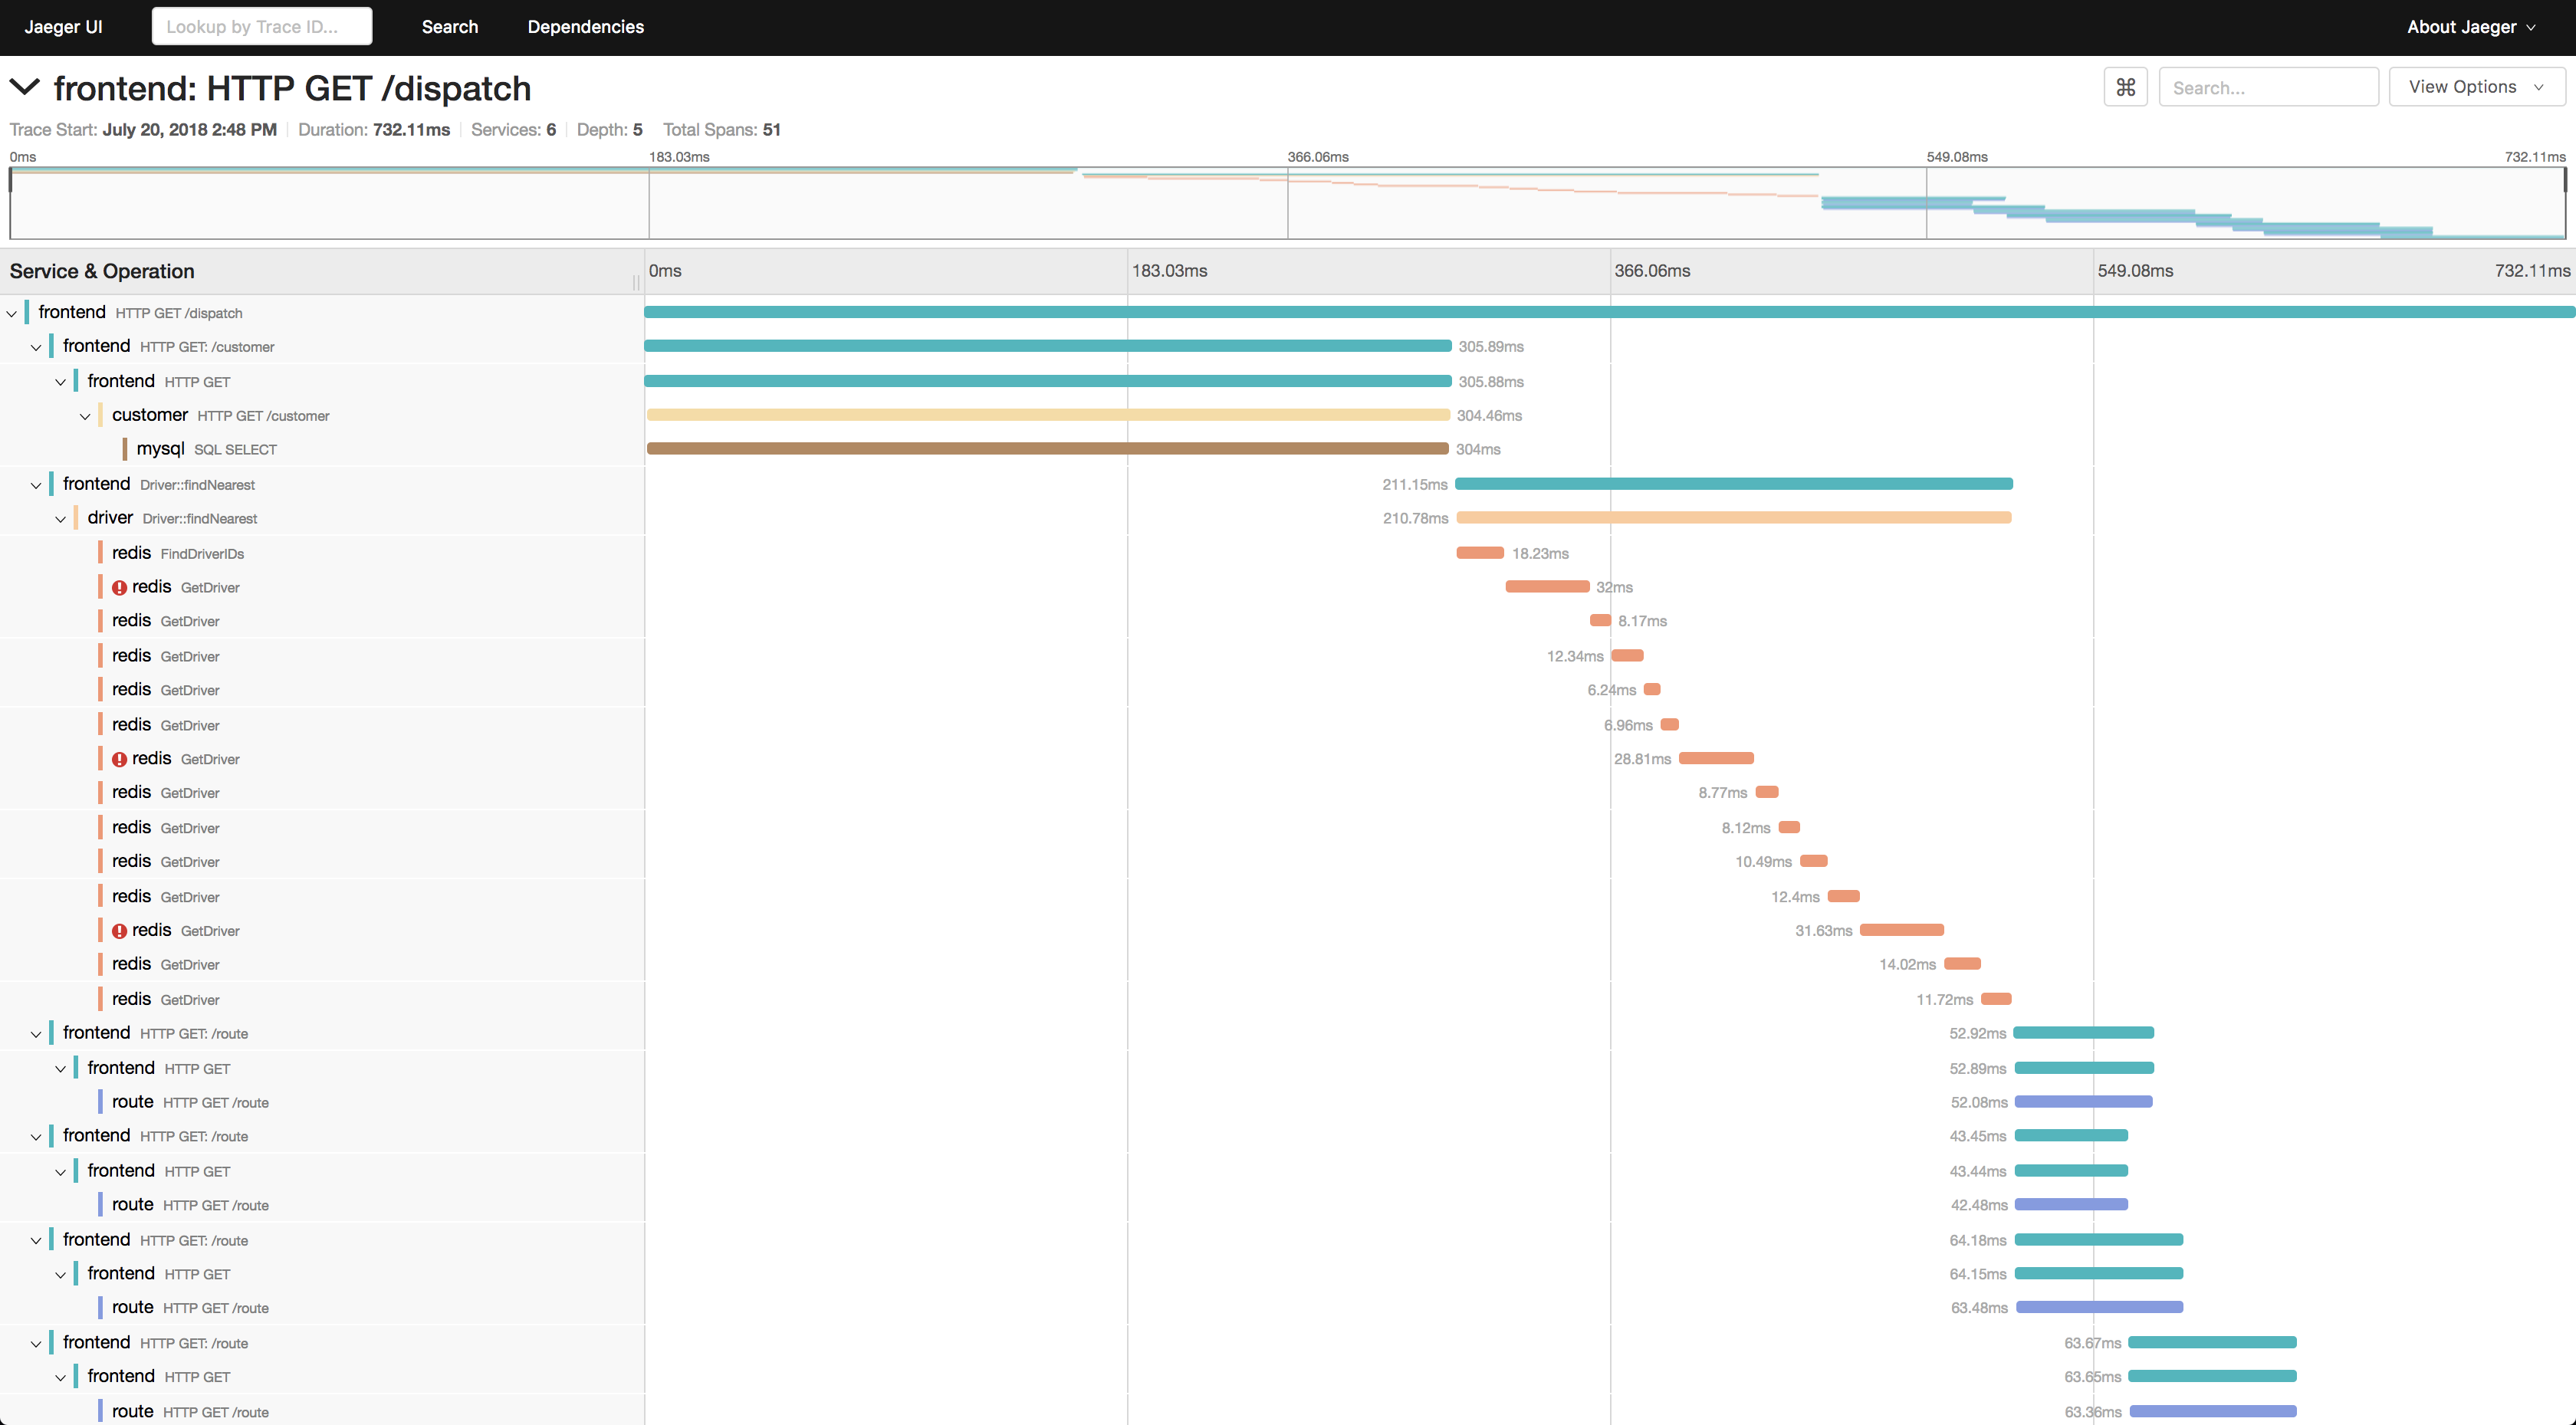
\includegraphics[width=1.0\textwidth]{myImages/trace-detail-ss.png}
\caption{Visualization of inter-service calls and timing data in Jaeger, by Jaeger Documentation under CC-BY-4.0 license}
\label{fig:jaeger_trace}
\end{figure}

As mentioned above, the distributed tracing pattern, similar to a service mesh, can be divided into two parts, an intrumentation or tracing part and the collection part.
Unsurprisingly, in order for a system to have distributed tracing capability, these two parts must be compatible, in other words, they must adhere to the same API specification.
In the open-source community, although there is no standardization yet, collective efforts such as OpenTracing\footnote{\href{https://opentracing.io}{https://opentracing.io}} tries to create a standardization of APIs, naming of concepts and shows tools such as Jaeger that complies with the OpenTracing standard.
Another major distributed tracing system is Zipkin\footnote{\href{https://zipkin.io}{https://zipkin.io}}, which supports distributed tracing integration with popular cloud frameworks such as Spring Cloud.

\subsubsection{Circuit Breaker}
\label{subsubsec:circuit_breaker}

From time to time, microservice instances may become unresponsive to other microservices, due to a high load that makes the service instance run out of resources, or a bug in the source code that makes the instance crash during run-time.
In a typical microservice application, the failure of microservice instances can be remedied by provisioning new ones, taking advantage of agile deployment capability thanks to fine-grained nature of the microservice architecture.
Nonetheless, in some cases, provisioning new instances of the failing microservice after the failure might not be good enough in terms of quality of service of the entire application.
As an example, if a call from the client side needs a service from a particular microservice and the request is routed to the failing microservice instance, the client would need to wait indefinitely, resulting in poor user experience.
In another and possibly more serious situation, if there are microservices that depend on the failing microservice instance, calls on the failing microservice might result in poor utilization of precious resources such as threads in other microservices, therefore causing poor performance and possible unresponsiveness in those client microservice instances as well, effectively cascading the original failure to other connected components in the system.
The circuit breaker pattern, in effect, intends to block a failure in a microservice instance from spreading to other instances in the rest of the system.
The mechanism of doing so is basically wrapping calls to a service and inspecting the result of call in terms of success or failure.
If there are enough failures, the circuit breaker component cuts the connection logically, or "trips" as the electrical circuit breaker does.
After that, all attempts to invoke the failing instance immediately returns an error for a specified period of time, so that the clients of the service do not wait or consume resources in a futile waiting mode.
The circuit breaker pattern can be implemented in either the client or server side, or it can have its own microservice instance as a proxy between them \cite{montesi2016circuit}.
Figure~\ref{fig:circuit_breaker} shows the three states found in the circuit breaker pattern and the flow between them.

\begin{figure}[H]
\centering
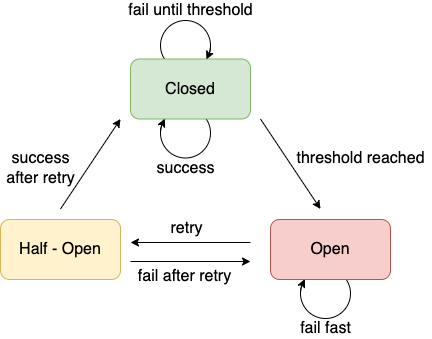
\includegraphics[width=0.60\textwidth]{myImages/circuit.png}
\caption{State diagram of circuit breaker pattern}
\label{fig:circuit_breaker}
\end{figure}

\begin{itemize}
    \item Closed State: The closed state is the normal state of operation in which the requests are conveyed to the invoked service. The number of cases, in which there is a erroneous return value from the called service or no return at all, is counted, and when the threshold is reached, the circuit breaker trips to the open state.
    
    \item Open State: In the open state, the requests are not conveyed and instead an immediate failure message is given back to the caller service. By means of periodically polling the failing service and checking if there is a successful return, or just waiting for a specified amount of time, the half-open state is reached.
    
    \item Half-Open State: The half-open state acts as an intermediary step before making the circuit closed and granting all requests admission to the invoked service. In this state, only a limited number of requests are permitted to the target service, while others are returned with an immediate error message. In case any of the limited calls made to the service fails, the circuit goes back to the open state. Lastly, if the limited calls are handled and returned successfully by the previously failing instance, the circuit becomes closed again, returning to the normal operation with counters being reset.
\end{itemize}

Example libraries that implement the circuit breaker pattern include Netflix Hystrix\footnote{\href{https://github.com/Netflix/Hystrix}{https://github.com/Netflix/Hystrix}} and Resiliency4j\footnote{\href{https://resilience4j.readme.io/docs}{https://resilience4j.readme.io/docs}} for Java, Opossum\footnote{\href{https://github.com/nodeshift/opossum}{https://github.com/nodeshift/opossum}} for Node.js and Gobreaker\footnote{\href{https://github.com/sony/gobreaker}{https://github.com/sony/gobreaker}} for Go languages.

\subsection{Anti-Patterns}
\label{subsec:antipattern}

% write which papers are used as a guide for this section

\subsubsection{Wrong Cut}
\label{subsubsec:wrong_cut}

As mentioned previously, microservices are designed using bounded context method, that is, each microservice is designed to carry out tasks related to one small business capability.
One misconception for the separation of microservices is the construction of microservices in a layered fashion, as opposed to assigning one business capability per microservice.
Designing microservices so that each microservice takes care of a major task from a technical perspective of the whole application is in fact a bad habit from SOA.
To explain shortly and to not repeat the differences between SOA and microservices architecture, it is appropriate to say that, while designing microservices in a layered style like UI, logic and data increases re-usability of both code and data, it conflicts with the requirements needed for the microservices architecture to deliver its benefits.
The wrong cut anti-pattern causes deployments to be dependant on other services, breaks team independence and brings about high-coupling, since each business task would then require more microservices to be available.
To avoid this pattern, microservices should be designed from a business perspective and the ownership of logic and data to a development team should be preserved.

\subsubsection{Nano Microservice}
\label{subsubsec:nano_microservice}

Another anti-pattern due to bad design choices in terms of separation of microservices is the nano microservice anti-pattern.
Unlike the wrong cut anti-pattern, the nano microservice anti-pattern does not stem from a misconception of the design paradigm but the excess use of separation of business boundaries.
As the name suggests, there might be cases that the microservices are designed so small that they cannot carry out business capabilities in a more or less indepedent way.
Designing microservices unnecessarily small results in a larger number of microservices in the system, and increases communication overhead.
This anti-pattern can also manifests itself as a cyclic dependency among a set of microservices, hinting at the fact that they are designed to be dependant on each other's logic or data to serve an outside request.
To remedy this anti-pattern, the nano microservices can be re-designed around business capabilites, aimed at one business capability per microservice.
In case of cyclic dependencies and frequent calls related to one business request, the microservices that take part in the related cluster or cycle can merged into a single microservice, while taking caution so that the new microservice does not become a megaservice.

\subsubsection{Mega Microservice}
\label{subsubsec:mega_microservice}

At the opposite end, there is the mega microservice anti-pattern, which means, designing one or more microservices in the system so that they can accomplish multiple business capabilities.
Having mega microservices in the application puts more work on the shoulders of the development team, and adding developers to the team leads to a situation that resembles a monolithic architecture.
It also results in additional difficulty in the deployment process, since in this case the part of system that changes in each deployment is larger, on contrary to one small microservice.
Again, it is important to design microservices in a way that each microservice performs one business capability.
Refactoring a mega microservice into a couple of microservices can help ease the deployment stage, and increase team independence.

\subsubsection{ESB Usage}
\label{subsubsec:esb_usage}

In Section \ref{subsec:diff}, the differences between the microservice and service-oriented architectures have been explained and particular roles each architectural paradigm assigns to the message broker component have been discussed.
Related to this difference, there is in fact an anti-pattern called ESB usage in the microservices world, that is based on the usage of ESB-like smart communication components in a microservice application.
The use of communication components that additionally takes care of service registry and discovery, transformation and some business logic contradicts with the "smart endpoints, dumb pipes" principle of the microservice architecture.
Rather than relying on the transformation of messages by an ESB, microservices should understand and handle different outlines of messages, register and discover services through a separate mechanism themselves.
Removing additional tasks such as these from the messaging component and using a lightweight message broker makes it easier to maintain the software and decreases the probability of a single point of failure case for the entire system.

\subsubsection{Hardcoded Endpoints}
\label{subsubsec:hardcoded_endpoints}

For a microservice to be able to make a request to another microservice, the requesting microservice need to know the location of the provider microservice.
The location of a microservice on the network is specificed via an IP address of its host and also a port number that is allocated for the process by the host in order to route network packets to the related process.
For that reason, to be able to communicate on the network, microservices need to know IP addresses and the port numbers of other microservices that they need to make a request to.
In short, there are two main methods to handle this task.
The first solution is to delegate this task of knowing which microservice is where on the network to a separate microservice or an underlying infrastructure designed for microservice architectures, namely, using the service registry and discovery design pattern.
The second way, however, is the anti-pattern that is about to be explained, the hardcoded endpoints anti-pattern.
The solution of the second way, and the poor one, is explicitly stating the addresses of microservices through different mechanisms, such as writing in the source code or storing them in a configuration file or environment variable.
Although this method can be used during the development process, it makes it harder to scale the services in the production stage, since it would be necessary to update all other microservice instances to know about the location of a new microservice deployment.
In addition, using hardcoded endpoints undermines the benefits of an internal load balancer, if one is used to distribute some share of the traffic of requests to a recently instantiated microservice.
Taking into consideration the promises proposed by the microservice architecture, it is quite beneficial and in some cases necessary to employ design patterns such as service registry and discovery that shapes the system in a way that allows those promises to be delivered.

\subsubsection{No API Gateway}
\label{subsubsec:no_api_gateway}

Similar to the two previous anti-patterns, the no API gateway anti-pattern is in fact the absence of a microservice design pattern, namely API gateway pattern.
Without an API gateway, clients of the microservice application need to communicate directly with the microservice that are needed for a particular task.
The clients have to know the location of multiple microservices and might have to send multiple requests for the resources they need.
The auxiliary tasks such as authentication, without an API gateway, are needed to be done for each microservice.
Last and probably the biggest difficulty of not having an API gateway is that the clients need to know how the application is structured, in other words, the names, locations and capabilities of microservices need to be conveyed to the client side.
For all these reasons, having an API gateway is of utmost importance for a microservice application to be able to communicate with the client in an effortless way.

\subsubsection{Shared Persistence}
\label{subsubsec:shared_persistence}

In Section \ref{subsec:chars}, while listing the general characteristics of the microservices architecture, it is stated that each microservice in general has its own persistence layer, meaning that each microservice deals with storing and managing its own data in its own database instance.
The shared persistence anti-pattern, as the name suggests, stem from using the same database record (entity, row or document) or the same database instance to serve requests from multiple microservices.
It is important to note that, unlike many of the previous anti-patterns, the shared persistence anti-pattern contains a spectrum of choices that can be made to decide the extent how much flexibility is desired at the cost of duplication of data and less efficient use of infrastructure resources.
Besides having one database instance per service, microservices can share a single database instance, a database schema in a database and even tables in a database schema.
While the use of a single database maximizes re-usability, private database schemes and private database tables allow for various degrees of data privacy and ownership, at the expense of possible data duplication and redundancy in the database instance.
In some cases, the decision to share data among multiple microservices may seem reasonable to developers and architects, however, it is crucial to remember that shared persistence anti-pattern diminishes team independence in the sense that changes to schema and table design need to be coordinated, hence increasing run-time coupling, since all microservices need a particular database instance to be up and running to serve a single business capability.

\subsubsection{Shared Libraries}
\label{subsubsec:shared_libraries}

Similar to the shared persistence anti-pattern, the shared libraries is a common anti-pattern in the sense that developers opt for sharing logic instead of data for this particular anti-pattern.
Extracting common code to a library is one of the best practices in software development discipline, since it reduces development efforts by following "Don't repeat yourself" (DRY) principle.
In addition, if there are multiple microservices on the same host, they can share a run-time library so that the resources of the host are best utilized.
However, sharing both development and run-time libraries can be detrimental to the independent development principle of the microservices architecture.
Because of sharing libraries, a change in the shared library requires careful coordination among teams, slowing down development speed in the long term. Furthermore, if the change is not coordinated well enough, an update on a shared library may cause significant changes in other microservices, potentially breaking the entire application.
As a remedy, the run-time libraries can be refactored into a separate microservice, so that if there is a need to change the library, the change can be incrementally introduced, in other words, there can be separate instances that support both versions, or the library can a have versioned API.
For the shared development libraries, developers should prefer code duplication instead of risking wrong abstraction so that the development efforts remain predictable in the future.

\subsubsection{No CI/CD Tools}
\label{subsubsec:no_cicd}

One of the main pillars of the microservices architecture is creating teams that develop microservices that handle one business capability.
The fine-grained decomposition allows teams to develop and maintain the microservice they own in an agile yet solid way.
To support the integration of development and operation tasks, teams are encouraged to use CI/CD tools, which allows for faster delivery without compromising software quality.
While it may seem easier to develop software without CI/CD tools at the first glance, the development and testing stage takes more time since a human agent needs to test the changed software part and possibly the whole software component, causing the time it takes to give feedback to developers to be longer.
On the other hand, having version control repositories for microservices, unit and integration tests in appropriate places, automated delivery mechanisms on successful commits and merges makes development faster and more under control.
Although the absence of CI/CD tools can also be disadvantageous for other software architectures, it is especially beneficial to use them in complex and modern architectures such as microservices so that the agility for microservice development can be achieved.

\subsubsection{Multiple Service Instances per Host}
\label{subsubsec:multiple_service_per_host}

For a microservices application, one of the deployment ways is deploying multiple microservice instances on a single virtual or physical host.
While this deployment option makes best use of resources of the underlying infrastructure, it severely harms the ease of scaling of services, since simply scaling a host results in all services that runs on the host to be scaled.
Moreover, different microservices may try to use different software components that runs on different OSs, or they can require different versions of the same dependency on the host machine, resulting in conflicting technologies and the need for a substantial amount of cooperation between teams during the development period.
In short, deploying multiple microservices on a single host is an anti-pattern and should be avoided in a microservice architecture.

\subsubsection{No API Versioning}
\label{subsubsec:no_api_versioning}

When a new version of a microservice is deployed, the developers may also decide to introduce a modified version of the former API, if it has been seen as a better fit for the newer version of the microservice.
In order not to break the communication between the altered microservice and other microservices, from time to time it is necessary for the altered microservice to support both the new and the old versions of its API, until other teams make changes required in their code that adopts the new API.
In cases such as these, API versioning can help identify the version of the API to be used between the client and the modified microservice.
The version of the API can be inserted in the URL path to be used by the client, or inserted as one of the custom headers in the HTTP request.
In addition, the degree of the change made to the API can be clarified to some extent, by using semantic versioning method.
The teams can coordinate and agree on a particular way of interpreting version numbers, or they also can make use of standization efforts such as SemVer\footnote{\href{https://semver.org}{https://semver.org}}.
In summary, utilizing API versioning is simple yet rewarding practice for microservices applications and not doing so may lead to inefficient communication efforts between teams.

\subsubsection{No Health Check}
\label{subsubsec:no_health_check}

Microservice applications may contain dozens of microservice instances, and for this reason, a failure or a crash in a microservice instance does not necessarily lead to an entire system-wide breakdown, making the failure hard to notice.
Not implementing a health check API endpoint in microservices or utilizing the related health check feature of the underlying container orchestration platform such as the one from Kubernetes is not just a trade-off but an anti-pattern in microservice architectures.
Specifying periodic health check in the orchestration platform or adding a couple of simple health check logic into request handling code of microservices is a valuable investment that can help monitor the whole application, making it easier to find and fix the service instance down or route requests to up-and-running instances until the problem is solved.

\subsubsection{Local Logging}
\label{subsubsec:local_logging}

Another bad practice that makes microservice applications less transparent to the developers is local logging anti-pattern.
Although implementing a distributed logging service is not trivial, say, compared to adding a health check endpoint, because of the significant disadvantages it causes in applications with large number of microservices, solely storing logs locally per microservice basis constitutes an anti-pattern.
Without a log aggregation mechanism, analyzing the state of the application requires more time and unimaginable effort in cases where the logs are larger in size and number.
In consequence, having a distributed logging structure in staging and production environments reduces trouble-shooting efforts and helps with monitoring processes.

\section{Summary}
\label{sec:state_of_the_art_summary}

In summary, the microservices architecture promotes the division of the application domain into bounded contexts and small business capabilities, carried out by one microservice per bounded context in general.
Each microservice is treated as a small software product that is designed, implemented and maintained by a small cross-functional team. Unlike SOA, the communication agent between microservices should perform plain and simple message distribution, without additional capabilities such as transformation of messaging format depending on the sender or receiver microservice or integration of services into the application.
For these infrastructure-related or auxiliary tasks, instead of having a central service that takes care of these duties, microservices application should have separate helper service instances, either through deploying these services themselves or using the ones offered by cloud platforms.
As an example, rather than collecting remote procedure call data between microservices thanks to an intelligent message broker, microservices should have a separate distributed trace collector service (such as Zipkin or Google Cloud Trace) in the system, and integrate themselves with the collector service by having a client SDK (such as Jaeger Client or Google Stackdriver Agent) in the microservice source code.
\\
To solve the common problems faced in microservices architecture, there are numerous approaches that vary in quality.
Choosing the right ones and implementing the design patterns related to the task at hand can help improve the quality of the architecture and hence quality of the service to end-users.
On the other hand, having anti-patterns in the application harms the independence of services and teams, diminishes the ease of scaling of individual services and results in poor developer experience and unsatisfactory end-users.
\\
As one can notice, there are quite a number of design patterns and anti-patterns about microservices architecture.
Utilizing the design patterns and avoiding the anti-patterns, in short, keeping in mind both kinds of practices might be intimidating from a practitioner's point of view who is new to microservices.
For this reason, we develop two research questions about these practices.
In the first one, we take a look into the literature to see if there exists a common classification regarding patterns and anti-patterns, that may help microservices practitioners and enthusiasts learn, embrace or avoid the practices, in the sense that the classification provides some structure of these practices, gathers similar ones into groups from some kind of perspective, making it easier for people to connect dots of microservice principles.
In case there is no consensus regarding patterns and anti-patterns, we aim to develop and propose a classification that we think may help people in the microservices area.
In the second research question, we change our perspective from literature to open source microservice applications and try to check and verify the use of the design patterns and the occurrence of the anti-patterns.
By doing so, we intend to see the level of correspondence between the "theory" and "practice" regarding these practices, in addition to providing example cases of design patterns and anti-patterns.

\chapter{Research Methodology}
\label{ch:research_method}%

In this chapter, the work conducted is described.
First, the research questions constructed for the study are introduced and in the next section, the methodology used to answer those research questions are explained.

\section{Research Questions}
\label{sec:research_questions}

For the scope of this study, the following two research questions have been established.

\begin{itemize}
    \item \textbf{RQ1}: Is there a consistent categorization or classification of design patterns and anti-patterns of microservices architecture in the academia?
    If not, what could be an alternative way to structure those design patterns and anti-patterns?
    
    \item \textbf{RQ2}: Which of these design patterns and anti-patterns exist in popular open source microservices applications?
\end{itemize}

Through these two research questions, the goal of this study is to see the level of sophistication and finesse in which the microservice design patterns and anti-patterns are categorized in the academia, propose a classification in case there is no consensus and to validate the occurrence of microservice design patterns and anti-patterns mentioned in the academia on a limited set of open source microservice projects.

\section{Adopted Methodology}
\label{sec:adopted_method}

\subsection{Methods Adopted for Research Question 1}
\label{subsec:adopted_method_RQ1}

To answer first research question, the following steps have been adopted.

\begin{itemize}
    \item First of all, in order to find out whether there exists a consistent classification of microservice design patterns and anti-patterns, research papers about the topic have been investigated.
    Digital libraries such as IEEE Explore, ACM Digital Library, Springer, Scopus, and the literature research tool, Google Scholar, have been consulted.
    The keywords used in the search queries made to the libraries included "microservice pattern", "microservice pattern classification", "microservice anti-pattern" and "microservice anti-pattern classification".

    \item After initial review of the studies found, few more studies have been added through snowballing technique, and from this extended set, the studies that do not contain a classification or grouping of patterns and anti-patterns have been eliminated.
    The studies found in this step have been labeled as primary studies.
    
    \item To be able to propose a classification of patterns and anti-patterns on a sound basis, various perspectives through which microservice architectures can be examined needed to be identified.
    For this reason, the systematic mapping studies found in the literature review process have been consulted.
    Because these studies do not bring a classification, they have been labeled as secondary studies.
    
    \item The contents of primary and secondary studies that are related to RQ1 have been summarized and under the light of findings a classification proposal is developed in Chapter \ref{ch:classification_result}.
\end{itemize}

\subsection{Methods Adopted for Research Question 2}
\label{subsec:adopted_method_RQ2}

Regarding the research method for the second research question, the work provided in the steps below have been conducted.

\begin{itemize}
    \item As a first step, open source projects implemented with a microservice architecture are searched in the repository hosting service GitHub.
    The keyword pattern "microservice OR micro-service" have been utilized.

    \item The search result are sorted using "most stars" sorting option.
    The rationale behind this decision is to see both the "text-book" microservice application examples provided by software companies and other projects that are potentially being used for microservice architecture reference.
    Although this decision does not necessarily result in a set of very high quality microservice applications with various design patterns implemented to solve microservice challenges, it is helpful in identifying the projects that has some visibility among the open source community and the patterns and anti-patterns that exist in those projects.
    
    \item The number of projects to be examined is selected as ten and accordingly ten microservice applications implemented either as a case study from software companies or example applications from individuals or group of developers have been selected.
    The repositories that are software development tools implemented to aid in microservice application development, such as frameworks, libraries, tool-kits and microservice application templates are excluded.
    Additionally, the repositories that include microservice term but implemented as examples of other architectures, or application repositories that do no have the source code but only the readily-built Docker images are excluded, since neither kinds of applications are suitable for the investigation to be conducted.
    
    \item Because of the technological heterogeneity that exist in both individual microservices in a microservice project and in the set of microservice projects to be examined, two design patterns, namely "saga" and "shared libraries" which require a competent understanding of the programming language being used and a thorough comprehension of the business logic are excluded from the list of patterns and anti-patterns to be identified.
    
    \item For the detection of other design patterns and anti-patterns, manual inspection of the source code of the application has been carried out, and if available, explanation of the application in terms of technologies involved in the repository has been consulted.
    The reason automated code analysis has not been utilized is that, the projects are implemented using various languages, libraries and frameworks, so there are a number of ways these patterns and anti-patterns can exist, such as through annotations in source code or including a ".yaml" or similar file that is related to the pattern.
    By inspecting a dependency management file (e.g., "pom.xml") to check if the library that implements a particular feature is utilized would not simply work for all kinds of pattern and anti-patterns.
    Furthermore, the way a pattern is implemented in a particular language or framework has not been known prior to the actual inspection of the project for all kinds of patterns, and through consulting to the documentation of the library or framework, the particular use of the library has been recognized in the examined application.
    The methods of detecting patterns and anti-patterns are explained in more detail in Section \ref{subsec:adopted_method_OS}.
\end{itemize}
    
\subsection{Methods Adopted to Detect Patterns and Anti-Patterns in Open Source Projects}
\label{subsec:adopted_method_OS}

Below, the methods used to detect patterns and anti-patterns have been described.

\paragraph{API Gateway} We checked the presence of a separate non-business microservice that makes calls to business microservices depending on the incoming requests, in cases where the connection to other services can be detected in source code of API gateway.
For applications that use a third-party API gateway component, we simply looked for a ".yaml", ".json", ".settings" or any similar file that involves routing logic rules, which mostly depend on the URL of the requested resource.

\paragraph{Service Mesh with Sidecar} We looked for dependencies that suggests the use of a common sidecar implementation, such as Linkerd, Envoy and Istio.
We searched for those sidecar names in the source code, and examined repository to check whether there are deployment instructions to "turn on" those sidecars on a specific deployment platform.

\paragraph{Service Registry and Discovery} The service registry and discovery pattern had two main ways to be utilized in the application, either through the use of a common service registry component (e.g., Eureka) or by delegating this mechanism to the infrastructure such as Kubernetes.
In cases where Eureka is used, we examined source code of microservices to check if there are necessary code or annotation related to the Eureka service discovery.
For cases that uses the service discovery of Kubernetes, we checked the service definitions inside Kubernetes ".yaml" files, that are constructed either on service basis or a single file that includes all service definitions.
For applications that use other infrastructures such as Docker Compose, Dapr, and Docker Swarm, we checked if the infrastructure provides service discovery in scenarios where the application is to be deployed on a multi host platform, by consulting official documentations and software forums.
As a result of the research on this issue, we concluded Dapr and Docker Swarm provides service discovery if the services are deployed on multiple hosts, while Docker Compose networking is only useful if the services are deployed on the same host.

\paragraph{Backends for Frontends} We looked for business services that have similar names and are related to the same business domain in the system, that might be implemented or configured in a slightly different way.

\paragraph{Asynchronous Messaging} We checked the source code of services to see if there is the notion of events/messages/channels in the business logic, and the presence of a message broker instance that the business microservices connect to in the application, without diving deep in the business logic of the entire system.

\paragraph{Database per Service} We checked if the business microservices have their own database instances, by checking the number of database instance definitions in Docker/Kubernetes files that deploy the whole application.
If most of the business microservices had their own database instances, and the microservices are not provided with the connection strings to other databases except for their own database instance, we concluded that the application has database per service pattern.

\paragraph{API Composition} For the API composition pattern, in order to not misjudge and state the status of presence correctly, we decided to look only for API composer or aggregator services, which serve API endpoints that combine responses from multiple business microservices.
The reason we omitted the inspection for API composition in the source code of business microservices is that, it would require understanding the business logic of the application, which might be doable for some small applications but would require a substantial amount of time and effort for applications that have, for example, nine or ten microservices which also use business abstractions or data-transfer objects provided by the utilized framework.
To spend less time on the business aspect of applications and to look for more patterns and anti-patterns in more projects, we made no observation about API composition that is part of the business logic in business microservices and conclude that the application utilizes API composition pattern only if the architecture involves a separate API aggregator service.

\paragraph{CQRS} We looked for microservices that deal only with query or command tasks, by inspecting the business logic of the services. 
Additionaly, we searched for keywords "command", "query" and "handler" to see if a mechanism similar to CQRS has been implemented in the source code, possibly in the endpoint handlers of services.

\paragraph{Event Sourcing} To detect event sourcing pattern, we first looked for an event store instance, which might be a database instance itself or might be a service that is featured as an event store and acts as wrapper or proxy to the stand-alone database.
Then, we checked if there is a connection from business microservices to event store and if the services use the notion of events.

\paragraph{Service Instance per Virtual Machine} We investigated the repository of the application to see if it includes VM-images, such AWS AMI or images for any other cloud provider, or any instruction for how to deploy the application using VM image per service method.

\paragraph{Service Instance per Container} We checked if the repository contains Docker or Kubernetes files, which would result in, by applying them through tools such as "docker-compose" or "kubectl", one container instance per service.

\paragraph{Serverless} We simply checked if the repository contains instructions for serverless deployment as one of the possible deployment approaches.

\paragraph{Health Check} With the help of keyword-searching (keywords such as "health", "check", "hc" "healthz"), we examined the source code of microservices to see if they implement health endpoints manually, or use automatic health endpoint feature of frameworks, for example by calling "addHealthChecks()" method of some interface provided by a framework.
In addition to the health endpoints of services, we checked if those endpoints are indeed probed by a monitoring service, for example, defined in Kubernetes .yaml files as "liveness" or "readiness", or a separate "status" service that periodically calls those health endpoints.

\paragraph{Distributed Tracing} Similar to health check method, we looked for trace generator libraries in source code and dependency files of services.
To conclude the presence of distributed tracing pattern positively, we also checked if the architecture contains a trace collector such as Zipkin or Jaeger.
In cases the microservices are instrumented with trace generators but the architecture does not contain a trace collector service, we checked if the trace generators are compatible with any cloud provider trace collector component, and if compatible, we concluded positively by justifying that the application is distributed-tracing-ready in a cloud environment.

\paragraph{Log Aggregator} Similarly, we checked for structured logging libraries in the source code of services manually and for the presence of a log aggregator service in the architecture.
Because the microservices are in general deployed to cloud platforms, to benefit from scalability in the best possible way, we also concluded positively if the application is ready for log monitoring component of a cloud platform.

\paragraph{Circuit Breaker:} For the circuit breaker pattern, we manually inspected the source code of services to see implementation or use of a circuit breaker library.
In our criteria, we also checked for possible circuit breaker mechanism definition in the deployment on a service mesh scenario, if the service mesh ".yaml" configuration files are provided in the repository.

\paragraph{Wrong Cut} To detect the wrong cut anti-pattern, we checked whether the microservices are designed around domains that are similar to actual business aspects or divisions that might be found in an application related to that area of expertise.
We checked the names of services and examined the source code to see whether one service is all about logic while some other service only deals with persistence tasks of multiple business services.
For user interface tasks, we did not count the presence of a single frontend service as wrong cut anti-pattern, as separating also the user interface components per business domain is not a must-have for microservice architectures.
Concerning this, there is also the "micro-frontends"\footnotemark[62]\footnotetext[62]{\href{https://micro-frontends.org}{https://micro-frontends.org}} paradigm which takes microservice mindset also to frontend components in a way that is not always present in microservice applications.

\paragraph{Nano or Mega Microservice} As for the imbalance in terms of business tasks, we simply judged the design of the application in a subjective way.
Again, without trying to go deep and understand the business logic of all services, we checked for services that have much more or much less endpoints than other services to be able to state the service is a candidate for nano or mega microservice anti-pattern.
Because the applications are exemplary applications, in general, the business services were expected to consist of simple endpoints such as "get all items" or "get item by ID".
In these cases, we did not conclude that the microservice is a candidate for nano microservice anti-pattern, as the logic is not quite imbalanced considering the other business microservices have similar logic and the scope of the application is small in general.

\paragraph{ESB Usage} We checked whether the implementation contains a ESB component such as NServiceBus\footnotemark[63]\footnotetext[63]{\href{https://particular.net/nservicebus}{https://particular.net/nservicebus}}, Apache Camel\footnotemark[64]\footnotetext[64]{\href{https://camel.apache.org}{https://camel.apache.org}} or Tibco Enterprise Message Service\footnotemark[65]\footnotetext[65]{\href{https://www.tibco.com/products/tibco-enterprise-message-service}{https://www.tibco.com/products/tibco-enterprise-message-service}}, instead of simpler message brokers such as RabbitMQ or Kafka.

\paragraph{Hardcoded Endpoints} For hardcoded endpoints, we checked for hardcoded IP address and port number pairs that are used to locate services from one service or through configuration files.
The port numbers are manually found in most cases inside Docker or Kubernetes files.
For IP addresses, we opted for simple regular expression "\textbackslash b\textbackslash d\{1,3\}\textbackslash .\textbackslash d\{1,3\}     \textbackslash .\textbackslash d\{1,3\}\textbackslash .\textbackslash d\{1,3\}\textbackslash b"
that finds four numbers up to three digits separated by dots, such as "0.0.0.0" but also "999.999.999.999", since there was already few items in the search result.
We inspected the found cases to see if it is indeed related to a bad practice about service discovery, and omitted cases where the IP addresses such as "0.0.0.0" and "127.0.0.1", in addition to word "localhost", are used in tests for the individual microservices, or for starting servers and binding them to localhost inside Docker containers.
In short, we tried to inspect the use of hardcoded IPs and port numbers in a way that separates the cases where they are used to by-pass the service discovery mechanism from cases where they are used for testing or legitimate server starting code from the point of view inside the Docker container.

\paragraph{Shared Persistence} To detect shared persistence anti-pattern, we checked whether there are connections to the same database instance from multiple microservices.
To inspect connections, we manually looked for the same connection string to the same database instance provided to microservices as environment variables, which are defined in Docker or Kubernetes .yaml files or any other file in case these tools are not utilized.

\paragraph{No CI/CD} We inspected the repository if there is a display of development status, as in a sign or statement about build or test status of the accepted pull request.
In addition, we checked the repository for folders or files that might include scripts that define the CI/CD pipeline, through one of the common CI/CD tools.

\paragraph{Multiple Service Instance per Host} Regarding this anti-pattern, since there is no way that we know of that prevents developers to deploy all microservices to the same host, we decided to check if there are conditions in the repository that might compel or "pressure" developers to deploy multiple services on the same host.
For this reason, we checked the containerization of services and see if there are cases that containerize multiple services or components to the same Docker image, which might be a result of a misunderstanding about microservice architecture paradigm.
In short, if the services have their own Docker image and do not share the image with other services, we concluded there is no multiple services per host anti-pattern, even though individual containerization does not prevent the actual bad practice.

\paragraph{No API Versioning} We manually checked API endpoints in the source code of services and API gateway component to see whether the URL contains "/v1/" or any similar substring.

\paragraph{No Health Check} We considered the presence of a health check pattern in the application and simply negated the result.
In case the health check pattern is implemented for a subset of services, we concluded that the pattern is utilized to some degree, as most of these applications are built for exemplary purposes, and concluded that there is evidence about the concept and implementation of health check pattern in the application.

\paragraph{Local Logging} Similarly, we took into consideration the log aggregator pattern and negated its result.
As for the implementation for a subset of services, we followed the same reasoning that we did for health check aspect,
and concluded negatively for this anti-pattern even if only some of services send their logs to a log collector service instance.

\chapter{Results of Research Question 1}
\label{ch:classification_result}%

In this chapter we address Research Question 1. According to the methodology we described in Section \ref{subsec:adopted_method_RQ1}, we have conducted a literature review. We have detected that, while there exists many studies regarding one or more design patterns or anti-patterns of microservice architectures, few studies approach to the topic from holistic point of view, in other words, mention or conduct a study involving different kinds of design patterns and anti-patterns of microservice architectures. In this chapter we start presenting those papers that we have identified at the end of our literature review, after the inclusion of papers found using snowballing technique and exclusion of papers that do not present a taxonomy of patterns or anti-patterns. Then we highlight the differences between the various classifications and motivate the need for a new proposal that we present at the end of the chapter.

\section{Classification of Patterns and Anti-Patterns Papers}
\label{sec:class_papers}

The primary studies that has been used to answer the first research question are listed in Table~\ref{table:primary_studies}.

\begin{table}[H]
\centering 
    \begin{tabular}{|l p{28em} l|}
    \hline
    \rowcolor{bluepoli!40}
    \textbf{ID} & \textbf{Title} & \textbf{Format}\T\B \\
    \hline \hline
    P1 & Architectural patterns for microservices: a systematic mapping study \cite{TaibiD2018APfM} & Conference\T\B\\
    \hline
    \rowcolor{bluepoli!10}
    P2 & Deployment and communication patterns in microservice architectures: a systematic literature review \cite{KARABEYAKSAKALLI2021111014} & Journal\T\B\\
    \hline
    P3 & Patterns related to microservice architecture: a multivocal literature review \cite{valdivia} & Journal\T\B\\
    \hline
    \rowcolor{bluepoli!10}
    P4 & A pattern language for scalable microservices-based systems \cite{10.1145/3241403.3241429} & Conference \T\B\\
    \hline
    P5 & Actual use of architectural patterns in microservices-based open source projects \cite{8719492} & Conference\T\B\\
    \hline
    \rowcolor{bluepoli!10}
    P6 & Quality attributes in patterns related to microservice architecture: a systematic literature review \cite{9105640} & Conference\T\B\\
    \hline
    P7 & Microservices anti-patterns: a taxonomy \cite{Taibi2020} & Book chapter\T\B\\
    \hline
    \rowcolor{bluepoli!10}
    P8 & On the study of microservices antipatterns: a catalog proposal \cite{10.1145/3424771.3424812} & Conference\T\B\\
    \hline
    P9 & Towards a collaborative repository for the documentation of service-based antipatterns and bad smells \cite{8712355} & Conference\T\B\\
    \hline
    \rowcolor{bluepoli!10}
    P10 & Quality assurance for microservice architectures \cite{9522227} & Conference\T\B\\
    \hline
    \end{tabular}
    \\[10pt]
    \caption{Primary studies that contain classification of patterns or anti-patterns}
    \label{table:primary_studies}
\end{table}

A concise explanation of primary studies and their views on the categorization of microservice design patterns and anti-patterns are given below.

\paragraph{P1} P1 is a systematic mapping study that reports on the widely used microservice architecture patterns and presents a catalogue regarding the advantages and disadvantages of microservice patterns.
As a result, they establish three categories, namely "orchestration and communication", "deployment" and "data storage".
In the first category, they include "API gateway", "service discovery" and "hybrid" patterns, and in the second category, "multiple service per host" and "single service per host" patterns.
Lastly, in the data storage category, they add "database per service", "database cluster" and "shared database server" patterns.
The "hybrid" pattern is, according to their definition, is a combination of "API gateway" and "service discovery" patterns, and is similar to ESB used in service-oriented architectures, which is, in fact, presented as an anti-pattern in this study.
Next, P1 suggests "multiple service per host" as a microservice pattern, explaining its advantages and disadvantages, while in this study, it is clearly stated as an anti-pattern.
In addition, P1 presents several options in the data management spectrum, presenting every option as a pattern, although in this study, some options such as "shared database server" is counted as an anti-pattern.

\paragraph{P2} In P2, the researchers make a systematic literature review, exploring "deployment" and "communication" patterns in microservice architectures.
While the researchers do not attempt to study other kinds of microservice patterns, they list several microservice patterns in the two categories, hence the study was considered useful in regard to the selection of patterns into different categories.
In the "deployment" category, they present "serverless", "service instance per VM" and "service instance per container" approaches, while in the "communication" category, they list "synchronous communication", "publish/subscribe communication", "combination of HTTP and message queue", "asynchronous communication", "communication using binary protocols" and "point-to-point communication" patterns.
Although the patterns belonging to the "deployment" category are also presented as patterns in this study, some communication approaches presented as options such as "publish/subscribe" and "communication using binary protocols" are described as communication patterns in P2, suggesting that there can be different levels of granularity in the detail of patterns that can be viewed as separate design patterns by researches.

\paragraph{P3} The authors of P3 make a literature review of patterns related to microservice architectures and come up with group names encompassing design patterns.
The grouping is made by quality attributes and benefits associated with each pattern and the resulting group names include "data persistence", "communication", "entry point", "distribution", "fault tolerance" and "supplementals".
Moreover, the quality attributes used in grouping involves "maintainability", "reliability", "performance efficiency", "security", "compatibility", and "portability".
Similar to the different levels of treatment towards design patterns and finer techniques around patterns seen in P2, the researchers of P3 choose to state what is presented in this study as options and techniques as patterns.

\paragraph{P4} The researchers of P4 present a taxonomy of microservices architectural patterns and further investigates design patterns that might help software architects develop highly scalable systems.
The taxonomy in the paper includes "migration", "design", "mitigation", "IOT", "front-end", "back-end", "DevOps", "deployment", "communication", "behaviour" and "orchestration" as microservice architectural patterns.
Coming to the architectural patterns related to scalability, they propose three categories, namely, "load balancer patterns", "decomposition patterns" and "grouping patterns".
Finally, resulting from two-step filtering activity, they suggests three actual microservice patterns, each of which belongs to the aforementioned category respectively: "internal load balancer", "circuit breaker" and "container" patterns.

\paragraph{P5} The next study P5 investigates microservice design patterns first in the academia and then in the open source software platform GitHub.
The two authors of P4 in this separate study P5 uses the same classification names that they do in P4, and also differentiate between the design patterns that are also used in SOA and the design patterns that solely belongs to microservice architectures.
One observation about P5 is that the researchers leave out some of the categories while assigning design patterns into the categories.
As a result, the pattern categories "deployment", "mitigation", "communication", "migration", "orchestration" and "back-end" has a number of design patterns selected for those categories, even though the categories "design", "behaviour", "front-end", "DevOps" and "IOT" do not have any patterns inside these groups.

\paragraph{P6} The three authors of P3 investigate quality attributes in microservice patterns in the study P6.
While doing so, they use the same quality attributes and present the same grouping of microservice patterns from P3.

\paragraph{P7} In the study P7, the authors conduct a survey that involves developers and practitioners who have experience in microservice architectures and ask them about microservice anti-patterns and their perceived harmfulness.
The anti-patterns mentioned by developers are then divided into two main groups: "technical" and "organizational" anti-patterns.
The technical anti-patterns are further classified into "internal", "communication" and "others", while organizational anti-patterns are segregated into "team oriented" and "technology and tool oriented".
The first observation about P7 is that it includes the behavioral pitfalls that can be seen in companies trying to embrace microservices, which are not included in this study.
For the technical anti-patterns, the authors choose to categorize anti-patterns based on the number of microservices each anti-pattern directly affects, in other words, according to the authors, internal anti-patterns impact individual authors, while communication anti-patterns undermines the communication between microservices and other anti-patterns, namely "lack of monitoring", "shared persistence" and "wrong cuts" hurts more or less the whole system.

\paragraph{P8} The researchers of the study P8 conduct a literature review and examine open source microservice projects to find anti-patterns of microservice architectures.
As a result of the study, they find sixteen microservice anti-patterns and categorize them based on the development cycle of a microservice system.
The four categories of microservice anti-patterns the authors present in P8 are "design", "implementation", "deployment" and "monitoring".

\paragraph{P9} The authors of the study P9 conduct a systematic literature review and extract 36 service-based anti-patterns that can be found in both SOA and microservice architectures.
While categorizing anti-patterns, they choose to consider the levels of abstraction the anti-patterns impact in the system and propose the "business", "application" and "architecture" anti-pattern categories.

\paragraph{P10} In the study P10, the researchers present the bad practises found in microservice architecture, and in doing so, they try to differentiate anti-patterns of microservice architectures from architectural (bad) smells.
For example, while in this study, "hardcoded endpoints" and "shared persistence" are considered anti-patterns, P10 considers them as architectural smells, nonetheless stating that the difference is blurred.
For the anti-patterns, the authors refer to the study P8 and present the same anti-patterns under the same categories as P8.

\section{Analysis of the Classifications}
\label{sec:analysis_of_class}

Considering the studies and the classifications listed above, there exists 5 pattern-related papers (P1, P3, P4, P5, P6) that gives output to 3 different categorizations (those from P1, P3, P5), since the study pairs P3-P6 and P4-P5 are written by the same researchers and use the same classification of patterns, and P2 presents only the patterns that the authors have seen fit to be placed under "communication" and "deployment" categories.
In addition, although the literature review was limited to the studies presented in the academia, during the literature review phase, one classification from a microservice patterns blog appeared valuable to be considered.
The author of the book \cite{richardson_book}, in his blog \cite{blogtaxonomy}, divides microservice design patterns into three main "application", "application infrastructure" and "infrastructure" categories, and considers some of what is presented in this study as the finer techniques as patterns, which can be put into many smaller categories.
\\
With regard to the classifications of anti-patterns of microservices, it has been observed that 4 anti-pattern related papers (P7 to P10) bring 3 different classifications, as the authors of P10 refer to P8 and use the same classification.
\\
In the light of these findings, it can be concluded that, although there are studies that investigate a particular aspect of microservices and attempt to associate design patterns with that category, there does not exist a consistent classification of both the design patterns and anti-patterns of microservice architectures.
\\
In an attempt to develop another classification of microservice design patterns and anti-patterns, it is useful to take into consideration the names of the categories the patterns and anti-patterns are associated with in other studies.
For ease of reference, the names of the categories of patterns and anti-patterns, including those from P2 and excluding empty group names from P5, are presented in Table~\ref{table:category_names}. 

\begin{table}[H]
\centering 
    \begin{tabular}{|l p{27em} l|}
    \hline
    \rowcolor{bluepoli!40}
    \textbf{ID} & \textbf{Category Names} & \textbf{Type}\T\B \\
    \hline \hline
    P1 & Orchestration \& Coordination, Deployment, Data Storage & Pattern\T\B\\
    \hline
    \rowcolor{bluepoli!10}
    P2 & Communication, Deployment & Pattern\T\B\\
    \hline
    P3 \& P6 & Data Persistence, Communication, Entry Point, Distribution, Fault Tolerance, Supplementals & Pattern\T\B\\
    \hline
    \rowcolor{bluepoli!10}
    P4 \& P5 & Deployment, Mitigation, Communication, Migration, Orchestration, Back-End & Pattern\T\B\\
    \hline
    P7 & Technical: Internal, Communication, Others; Organizational: Team Oriented, Technology and Tool Oriented & Anti-Pattern\T\B\\
    \hline
    \rowcolor{bluepoli!10}
    P8 \& P10 & Design, Implementation, Deployment, Monitoring & Anti-Pattern\T\B\\
    \hline
    P9 & Architecture, Application, Business & Anti-Pattern\T\B\\
    \hline
    \end{tabular}
    \\[10pt]
    \caption{Names of pattern and anti-pattern categories used in related studies}
    \label{table:category_names}
\end{table}

From the category names presented in Table~\ref{table:category_names}, the concepts and aspects around which the authors categorize the patterns and anti-patterns can be inferred.
First of all, the classifications from P1, P2, P4 and P8 use the explicit "deployment" category for patterns and anti-patterns related to the deployment aspect of microservices.
When examined thoroughly, the "distribution" name used in P3 encapsulates techniques such as "container", "microservice DevOps", "self-contained services" and "enable continuous integration", in other words, the methods that aid in the deployment of microservice systems.
In regard to P7, the bad practises of deployment aspect of microservices is discussed under "organizational" and further "technology and tool oriented" anti-pattern category.
The wrong-doings in the deployment aspect is not discussed in P9 in detail, possibly because the study P9 aims to encompass anti-patterns in the traditional service-oriented architectures, and the deployment of SOA could be said to be more similar and follows more or less the deployment norms of monolithic systems.
\\
Another observation about the classifications is that the category "communication" is often used in the studies.
For those studies that do no explicitly use "communication" category, when examined in detail, it is observed that the communication aspect is dealt with in different categories.
For example, the communication aspect of microservices is mentioned to some extent in P1 under "orchestration \& coordination" category, although the term "orchestration" is more used in the community to imply infrastructure-related tasks, such as the ones Kubernetes can carry out.
While P9 does not use "communication" category, P8 places some anti-patterns that undermines the communication in a microservice system to some extent.
As an example, P8 puts "hardcoded endpoints" anti-pattern into "implementation" category and "no API gateway" anti-pattern into "deployment" anti-pattern category.
\\
The last commonality that could be observed from the classifications is that the classifications from P1 and P3 choose to use "data storage" and "data persistence" category names to emphasis those patterns related to the persistence aspect of microservices.
\\
As a side note, again, from the careful examination of studies, it has been observed that some classifications use particular category names that do not effectively convey the underlying aspect, benefit of patterns or harm of anti-patterns that are put into those categories. 
One exemplary case could be of P1 using "orchestration" category to present "service discovery" and "API gateway" patterns.
Another example about this point is that the study P5 presents "circuit breaker" under "deployment", "service discovery" under "migration" and "continuous integration" under "orchestration" categories, while P8 associates "no API gateway" under "deployment" anti-pattern category.

\section{Systematic Mapping Studies}
\label{sec:sys_map}

In order to aid the development of a classification for microservice patterns and anti-patterns, it can be beneficial to take a look at the studies that conduct systematic mapping studies.
The three papers listed in Table~\ref{table:secondary_studies} present a list of keywords that are gathered around similar concepts.

\begin{table}[H]
\centering 
    \begin{tabular}{|l p{30em} l|}
    \hline
    \rowcolor{bluepoli!40}
    \textbf{ID} & \textbf{Title} & \textbf{Format}\T\B \\
    \hline \hline
    S1 & A systematic mapping study in microservice architecture \cite{7796008} & Conference\T\B\\
    \hline
    \rowcolor{bluepoli!10}
    S2 & Microservices: a systematic mapping study \cite{10.5220/0005785501370146} & Conference\T\B\\
    \hline
    S3 & Towards a taxonomy of microservices architectures \cite{10.1007/978-3-319-74781-1_15} & Conference\T\B\\
    \hline
    \end{tabular}
    \\[10pt]
    \caption{Secondary studies about concepts and keywords in microservice architectures}
    \label{table:secondary_studies}
\end{table}

Short explanations about the parts found in these studies that could be helpful in development of classification are stated below.

\paragraph{S1} The authors of S1 present the challenges and quality attributes of microservice architectures that they discovered during their literature review that involves 33 studies.
The microservice challenges include "communication/integration", "service discovery", "performance", "fault-tolerance", "security", "tracing and logging", "application performance monitoring", and "deployment operations", any of which is tackled by one or more design patterns presented in this study.
Another observation that could be made about the findings presented in S1 is that the top six quality attributes mentioned in the literature are "scalability", "independence", "maintainability", "deployment", "health management" and "modularity", hinting at the fact that the emphasis on the microservice systems is that they are built as a set of small independent software products that are developed and maintained independently.

\paragraph{S2} The researchers in S2 extract keywords out of 21 studies and based on the results, it can be observed that the four most frequent key terms are "scalability", "independently deployable", "testing" and "architectural style", again, putting emphasis on the nature of microservice that microservices are a composition of small independently deployable software components.
Additionaly, as a result of the research, the authors of S2 states that they can distinguish two technical perspectives about the methods found in microservice architectures: "architecture" and "methods".
The "architecture" perspective encompasses architecture design and implementation methods, while "methods" perspective is more process-centric, according to the authors.

\paragraph{S3} Lastly, the author of S3 conducts a literature review and based on the 46 relevant primary work, proposes a taxonomy of concepts that exists in microservice architecture landscape.
The six core categories of the suggested taxonomy include "design", "implementation", "deployment", "runtime", "crosscutting concerns" and "organizational aspects".
In this taxonomy, the domain-related and architecture-related design tasks are placed under the "design" category, while data storage kinds (SQL or NoSQL), data exchange methods (REST or RPC) and service discovery methods are found  in the "implementation" category.
Next, the "deployment" category involves different options to where the code physically runs, such as cloud or in-house, and "runtime" encompasses the deployment approaches presented in this study, such as containers, virtual machines and serverless options.
The aspects that are in general considered supplementary techniques such as monitoring, testing and DevOps are divided into "crosscutting concerns" and "organizational aspects" category.

The first observation about the secondary studies is that there are indeed a number of ways the patterns and anti-patterns can be categorized.
Using challenge key terms directly from S1 would result in a large number of categories, although some challenges can be merged under a larger category.
The two perspectives "architecture" and "methods" from S2 sounds promising since the placement of patterns and anti-patterns could be intuitive, that is, whether a pattern or an anti-pattern belongs to architecture or methods category might be deduced from the size of the change it brings into the architecture.
For example, while the "service discovery" pattern makes a big change in the architecture, the "no health check API" anti-pattern is more process-centric hence belongs to the methods category.
On the other hand, the taxonomy of S3 uses the stages of microservice application development as categories and add supplementary methods into two new categories.

\section{A Proposal for a New Classification}
\label{sec:proposal}

Considering the classifications from primary studies and insights from secondary studies explained in detail above, we propose the taxonomy of patterns and anti-patterns in microservice architectures given in Table~\ref{table:pattern_table} and Table~\ref{table:antipattern_table}, respectively.
The important aspects valued during the development of the classification is that, first, we aimed at categories being more rigid in that one pattern or anti-pattern in a category do not influence the other categories much, whether it is a challenge, attribute or development stage in microservice architectures.
For example, having "asynchronous communication" pattern solely in "communication" category would be acceptable at first, however, when examined in detail, the mechanisms of utilizing an asynchronous communication might require a messaging pipeline or an event source that is capable of storing messages in queues, and would in turn influence how the application business domain is reflected in the implementation.
Another example could be of that using a separate "data persistence" category for the patterns and anti-patterns.
Our argument of not using any data-related category is that it also influences other parts of the system in a significant way.
To illustrate, having "event sourcing" or "CQRS" patterns or "shared database instance" anti-pattern in a data-related category would look good at first glance, although patterns such as "event sourcing" and "CQRS" considerably changes the architecture of the system, in the sense that those patterns change the ways and logical layers through which microservices communicate with each other.
While "event sourcing" and "CQRS" adds persistence mechanisms other than the norm of database-per-service pattern, "event sourcing" imposes the use of pub/sub mechanism for microservices to be able to benefit from it, and "CQRS" alters the way the front-end and back-end communicate, causing the front-end to use different data models based on the particular request.
As for the "shared database instance" anti-pattern, it relieves microservices from the constraint that they should communicate only through API calls, by their API definitions and not directly use the target data source.
\\
\begin{table}[H]
\centering 
    \begin{tabular}{ 
  | >{\centering\arraybackslash} m{12em} 
  | >{\centering\arraybackslash} m{12em} 
  | >{\centering\arraybackslash} m{12em} | }
    \hline
    \rowcolor{bluepoli!40}
    \textbf{Architectural Patterns} & \textbf{Deployment Patterns} & \textbf{Monitoring \& Reliability Patterns}\T\B \\
    \hline \hline
    API Gateway & Service Instance per Container & Health Check\T\B\\
    \hline
    \rowcolor{bluepoli!10}
    Service Mesh with Sidecar & Service Instance per VM & Distributed Tracing\T\B\\
    \hline
    Service Registry \& Discovery & Serverless & Log Aggregator\T\B\\
    \hline
    \rowcolor{bluepoli!10}
    Backends for Frontends &  & Circuit Breaker\T\B\\
    \hline
    Asynchronous Messaging & & \T\B\\
    \hline
    \rowcolor{bluepoli!10}
    Database per Service & & \T\B\\
    \hline
    Saga & & \T\B\\
    \hline
    \rowcolor{bluepoli!10}
    API Composition & & \T\B\\
    \hline
    CQRS & & \T\B\\
    \hline
    \rowcolor{bluepoli!10}
    Event Sourcing & & \T\B\\
    \hline
    \end{tabular}
    \\[10pt]
    \caption{Proposed Classification of Microservice Design Patterns}
    \label{table:pattern_table}
\end{table}
\\
\begin{table}[H]
\centering 
    \begin{tabular}{ 
  | >{\centering\arraybackslash} m{12em} 
  | >{\centering\arraybackslash} m{12em} 
  | >{\centering\arraybackslash} m{12em} | }
    \hline
    \rowcolor{bluepoli!40}
    \textbf{Architectural Anti-Patterns} & \textbf{Deployment Anti-Patterns} & \textbf{Monitoring \& Reliability Anti-Patterns}\T\B \\
    \hline \hline
    Wrong Cut & No CI/CD & No Health Check\T\B\\
    \hline
    \rowcolor{bluepoli!10}
    Nano Microservice & Multiple Service Instances per Host & Local Logging\T\B\\
    \hline
    Mega Microservice & No API Versioning & \T\B\\
    \hline
    \rowcolor{bluepoli!10}
    ESB Usage &  & \T\B\\
    \hline
    Shared Libraries &  & \T\B\\
    \hline
    \rowcolor{bluepoli!10}
    Hardcoded Endpoints & & \T\B\\
    \hline
    No API Gateway & & \T\B\\
    \hline
    \rowcolor{bluepoli!10}
    Shared Persistence & & \T\B\\
    \hline
    \end{tabular}
    \\[10pt]
    \caption{Proposed Classification of Microservice Anti-Patterns}
    \label{table:antipattern_table}
\end{table}
The reason why an "implementation" category is not used, although it is for sure one of the stages of typical software development and could be used for a category, is that, we argue that points illustrated in "implementation" categories are actually indications related to other groups or concepts.
For instance, the "hard-coded endpoint" and "shared libraries" anti-patterns given in P8 are the result of bad architectural design choices, in the sense that the first is the direct result of the absence or neglect of the "service discovery" pattern, and the second is related to a bad design decision about whether a common logic should be employed as a library or a microservice, and not necessarily an original wrong-doing that show up during the implementation phase.
One counter-argument claiming that the "hard-coded endpoint" anti-pattern is still related to the implementation category might be that, even though a service discovery mechanism is utilized in the system, developers can hard-code endpoints and by-pass the service discovery for some of the microservices.
About this argument, we argue that the same can be true as well for many other design decisions, and not obeying the design and not implementing microservices accordingly should count as implementation anti-patterns for each of the design decision in a trivial manner.
We claim that creating a separate implementation anti-pattern for each design decision serves no purpose for research purposes other than cluttering the landscape, and it is a reasonable assumption to make that the benefits and drawbacks of options stated in this study are only valid if they are executed or chosen to do so.
\\
For the reasons stated above, it has been seen fit in this study to merge main topics such as communication, data, design and implementation into one main category called "architectural design" patterns and anti-patterns, similar to the categorization used for techniques related to microservices in systematic mapping study S2.
For the techniques that are more process-centric, we have chosen to split the remaining patterns and anti-patterns into two method-oriented categories, namely "deployment" and "monitoring \& reliability".
While the "deployment" category is also used by other studies, we have seen it suitable to merge the challenges "tracing and logging", "application performance monitoring" and "fault-tolerance" presented in S1, into the "monitoring \& reliability" category.
We believe that this classification is also intuitive in the sense that it reflects the deployment and maintenance periods of a software product lifecycle, hence might be more useful for developers to see all kinds of patterns and anti-patterns during a particular step of software development period.
Inside the "deployment" category, in addition to the deployment options such as "service instance per container" and "serverless", the pitfalls "no CI/CD" and "no API versioning" have been judged appropriate to be placed under "deployment" anti-patterns since they occur during the deployment stage, the first tool not being utilized to make the deployment more frequent and the second is a bad practice when developers change the API definition between the two releases of a microservice.
As for the "monitoring \& reliability" category, the patterns and anti-patterns that helps or undermines the actual capability and continuity of serviceability have been considered relevant to be placed.
\\
Effectively, the proposed taxonomy merges the inter-related topics such as communication, data and architectural design into one "architecture" category and presents "architectural patterns" and "architectural anti-patterns" categories, and then gather the process-centric techniques and pitfalls into the four "deployment patterns", "deployment anti-patterns", "monitoring \& reliability patterns" and "monitoring \& reliability anti-patterns".


\chapter{Results of Research Question 2}
\label{ch:pattern_result}%

To investigate the occurrence of patterns and anti-patterns of microservice architecture in open source microservice projects, ten microservice project repositories on GitHub have been identified.
The list of projects examined are given in Table~\ref{table:project_list}, with the number of GitHub stars that indicates to a certain degree that the projects have significant visibility to the practitioners.

\begin{table}[H]
\centering 
    \begin{tabular}{ 
  | >{\centering\arraybackslash} m{2em}
  | >{\centering\arraybackslash} m{19em} 
  | >{\centering\arraybackslash} m{11em}
  | >{\centering\arraybackslash} m{3.5em} | }
    \hline
    \rowcolor{bluepoli!40}
    \textbf{ID} & \textbf{Repository Name} & \textbf{URL} & \textbf{GitHub Stars}\T\B \\
    \hline \hline
    R1 & dotnet-architecture/eShopOnContainers & \href{https://bit.ly/3uQzv6e}{https://bit.ly/3uQzv6e} & 20.3k\T\B\\
    \hline
    \rowcolor{bluepoli!10}
    R2 & GoogleCloudPlatform/microservices-demo & \href{https://bit.ly/3JrKOFX}{https://bit.ly/3JrKOFX} & 12k\T\B\\
    \hline
    R3 & sqshq/piggymetrics & \href{https://bit.ly/34GC4gv}{https://bit.ly/34GC4gv} & 11.5k\T\B\\
    \hline
    \rowcolor{bluepoli!10}
    R4 & cer/event-sourcing-examples & \href{https://bit.ly/3JqMeAz}{https://bit.ly/3JqMeAz} & 2.9k\T\B\\
    \hline
    R5 & microservices-patterns/FTGO-application & \href{https://bit.ly/3oPndHn}{https://bit.ly/3oPndHn} & 2.4k\T\B\\
    \hline
    \rowcolor{bluepoli!10}
    R6 & vietnam-devs/coolstore-microservices & \href{https://bit.ly/3v4YVgL}{https://bit.ly/3v4YVgL} & 2k\T\B\\
    \hline
    R7 & Crizstian/cinema-microservice & \href{https://bit.ly/3GOe3RC}{https://bit.ly/3GOe3RC} & 1.6k\T\B\\
    \hline
    \rowcolor{bluepoli!10}
    R8 & asc-lab/dotnetcore-microservices-poc & \href{https://bit.ly/3sE87FU}{https://bit.ly/3sE87FU} & 1.5k\T\B\\
    \hline
    R9 & elgris/microservice-app-example & \href{https://bit.ly/3sIn6i7}{https://bit.ly/3sIn6i7} & 1.4k\T\B\\
    \hline
    \rowcolor{bluepoli!10}
    R10 & aspnetrun/run-aspnetcore-microservices & \href{https://bit.ly/3pB7zjd}{https://bit.ly/3pB7zjd} & 1.1k\T\B\\
    \hline
    \end{tabular}
    \\[10pt]
    \caption{List of examined projects}
    \label{table:project_list}
\end{table}

Starting from the repository R1, the result of the examination is presented in the following pages.
First, a table that indicates the existence of each design pattern and anti-pattern for the project examined is prepared.
Then, a few sentences that explain the state of presence of each design pattern or anti-pattern in terms of implementation and libraries or frameworks used are provided. 

\section{R1: eShopOnContainers}
\label{sec:R1}

\subsection{Overview of the Application R1}
\label{subsec:R1_overview}

The first examined application is "eShopOnContainers" application, developed by Microsoft to provide use cases for .NET framework features implemented for microservice architectures.
As the name suggests, the application is intended to be an e-commerce application, involving four business microservices, namely "identity", "catalog", "ordering" and "basket" services.
In addition business services, the system contains an event bus, two separate API gateways for web and mobile clients, a web status service that conducts health checks and a log collector service.
Figure~\ref{fig:R1_arch} shows the architectural diagram of the application, adapted from the architectural diagram in the repository.

\begin{figure}[H]
\centering
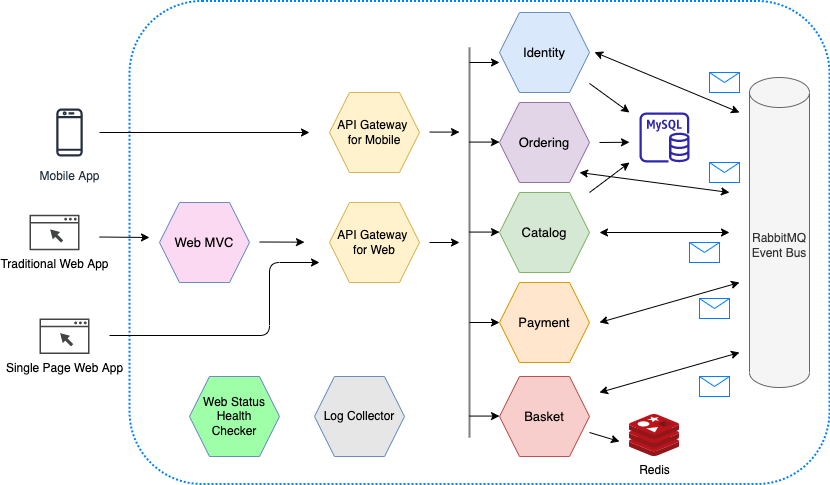
\includegraphics[width=1\textwidth]{myImages/R1.png}
\caption{Architectural diagram of eShopOnContainers application, adapted from diagram in repository under MIT license}
\label{fig:R1_arch}
\end{figure}

\subsection{Microservices Design Patterns and Anti-Patterns in R1}
\label{subsec:R1_detection}

As a result of inspection for design patterns and anti-patterns, we present Table~\ref{table:R1_result} which shows the presence of each pattern and anti-pattern in the application.

\begin{table}[H]
\centering 
    \begin{tabular}{ 
  | >{\centering\arraybackslash} m{16em} 
  | >{\centering\arraybackslash} m{2.2em} 
  | >{\centering\arraybackslash} m{16em} 
  | >{\centering\arraybackslash} m{2.2em} | }
    \hline
    \rowcolor{bluepoli!40}
    \textbf{Design Pattern} & \cmark \textbackslash – & \textbf{Anti-Pattern} & \cmark \textbackslash – \T\B \\
    \hline \hline
    API Gateway & \cmark & Wrong Cut & – \T\B\\
    \hline
    \rowcolor{bluepoli!10}
    Service Mesh with Sidecar & \cmark & Nano Microservice & – \T\B \\
    \hline
    Service Registry \& Discovery & \cmark & Mega Microservice & – \T\B \\
    \hline
    \rowcolor{bluepoli!10}
    Backends for Frontends & \cmark & ESB Usage & – \T\B \\
    \hline
    Asynchronous Messaging & \cmark & Hardcoded Endpoints & – \T\B \\
    \hline
    \rowcolor{bluepoli!10}
    Database per Service & – & No API Gateway & – \T\B \\
    \hline
    API Composition & \cmark & Shared Persistence & \cmark \T\B \\
    \hline
    \rowcolor{bluepoli!10}
    CQRS & \cmark & No CI/CD & – \T\B \\
    \hline
    Event Sourcing & – & Multiple Service Instances per Host & – \T\B \\
    \hline
    \rowcolor{bluepoli!10}
    Service Instance per VM & – & No API Versioning & – \T\B \\
    \hline
    Service Instance per Container & \cmark & No Health Check & – \T\B \\
    \hline
    \rowcolor{bluepoli!10}
    Serverless & – & Local Logging & – \T\B \\
    \hline
    Health Check & \cmark &  & \T\B \\
    \hline
    \rowcolor{bluepoli!10}
    Distributed Tracing & – & & \T\B \\
    \hline
    Log Aggregator & \cmark &  & \T\B \\
    \hline
    \rowcolor{bluepoli!10}
    Circuit Breaker & – &  & \T\B \\
    \hline
    \end{tabular}
    \\[10pt]
    \caption{Presence of microservice design patterns and anti-patterns in repository R1}
    \label{table:R1_result}
\end{table}

Below, the particular implementation of design patterns and explanations about anti-patterns are provided.

\paragraph{API Gateway} The application uses two API gateways, one for web applications in browsers and another one for mobile clients using Xamarin-based app.
The gateways are implemented using Envoy\footnotemark[66]\footnotetext[66]{\href{https://www.envoyproxy.io}{https://www.envoyproxy.io}} proxies, which routes incoming requests from clients to internal microservices based on the route of the particular HTTP request.
The routing rules are specified by "envoy.yaml" files, which matches the HTTP requests with string prefixes and routes requests to hosts specified in the same "envoy.yaml" file.

\paragraph{Service Mesh with Sidecar} Because of its complexity, the service mesh pattern is not employed throughout the eShopOnContainers application but only provided as a deployment option.
The required configuration files for configuring sidecars per microservice container are given as examples for two microservices, namely Linkerd "ServiceProfile" files "basket-api-sp.yaml" and "catalog-api-sp.yaml" files.
The remaining instructions to deploy the application on Linkerd service mesh (installing Linkerd and then deploying the application on Kubernetes and so on) are presented in the deployment section of the repository.

\paragraph{Service Registry and Discovery} The application is provided with both "docker-compose" yaml files, to deploy multiple containers on a single host, and Kubernetes yaml files, to deploy the containers on multiple hosts. 
The Kubernetes files are provided as Helm\footnotemark[67]\footnotetext[67]{\href{https://helm.sh}{https://helm.sh}} yaml files, which is a package manager that is used to create template yaml files, called "Helm charts", and values to be used in those templates for Kubernetes, so that the deployment specifications can be changed easily without creating multiple Kubernetes files or changing them manually.
In short, the application does not include a microservice for service registry and discovery purposes but uses the service registry and discovery features of the underlying deployment infrastructure.

\paragraph{Backends for Frontends} For mobile clients that use Xamarin mobile app and for web clients, there are two different API gateways and two different aggregator microservices.
While the routing rules for the API gateways are identical, the controllers for aggregator services are different, implying the fact that the returned data would be different based on the kind of the client.

\paragraph{Asynchronous Messaging} The application uses the concept of events as part of some of the logic involved and proposes two kinds of message queues.
For on-premise use cases, the microservices use a RabbitMQ instance to communicate about events, while for on-cloud deployment, instead of RabbitMQ, the application offers integration with Azure Service Bus.

\paragraph{Database per Service} Even though there is not an evidence detected that signals accessing the same data entry from multiple microservices, the three microservices "catalog", "ordering" and "identity" uses the same MySQL server instance to store their data, by creating their own database schema in the same database instance.
The only other microservice that involves data storing and accessing is the "basket" microservice and it utilizes Redis key-value store as another container instance.
At this point, it is important to note that this repository is created as an example to be tinkered by developers who are new to the microservice architecture and it is stressed by creators of this project in the Wiki page of repository that this decision is not ideal for microservice projects in production and is only taken to lower the infrastructure requirements for the application to let it run on also on hosts with lower computing resources.
Nonetheless, since the detection criteria for this pattern is set in this study such that each microservice that needs a data-related service should have its own database instance, it can be concluded that the database per service pattern is not employed in this application.

\paragraph{API Composition} As previously said, the application utilizes two aggregator services and the client requests that are data-wise complex are handled by those aggregator services.
Instead of regular HTTP requests, the aggregator services use gRPC protocol to communicate with "ordering", "catalog" and "basket microservices, take required data, execute logic to transform data into appropriate structure for response and respond to API gateways with HTTP responses.

\paragraph{CQRS} The CQRS pattern is utilized to some degree inside the "ordering" microservice.
The API definition of "ordering" service is divided into two command and query parts, where the command part involves commands and respective command handler classes, and the query part includes query classes that makes a connection to the database and returns the result.
In contrary to using different data models for command and query, the two parts read or write data through the same "OrderAggregate" data model.
The implementation of these classes are aided by MediatR\footnotemark[68]\footnotetext[68]{\href{https://docs.microsoft.com/en-us/dotnet/architecture/microservices/microservice-ddd-cqrs-patterns/microservice-application-layer-implementation-web-api}{https://docs.microsoft.com/en-us/dotnet/architecture/microservices/microservice-ddd-cqrs-patterns/microservice-application-layer-implementation-web-api}} library, created to help implement CQRS and mediator patterns in .NET platforms.

\paragraph{Event Sourcing} Although the use of event concept is detected in the application, the architecture is not constructed in a way that there exists a separate event store for microservices to send and consume events.

\paragraph{Service Instance per Virtual Machine} The repository does not include service instance per VM as a deployment option with readily-built VM images.

\paragraph{Service Instance per Container} The application utilizes one microservice instance per container deployment pattern as the default deployment method.
The containers can be instantiated locally using Docker Compose or Kubernetes or deployed onto cloud using Azure Kubernetes Service or any other Container-as-a-Service platform.

\paragraph{Serverless} Even though integration with Azure Functions is provided in a few sentences, the application is neither ready nor suitable to be deployed to a serverless environment since the microservices involved work with databases and replacing those databases with persistent cloud resources would not be trivial.

\paragraph{Health Check} The microservices use built-in health monitoring feature of .NET platform and implement health check endpoint "\textbackslash hc" and liveness endpoint "\textbackslash liveness" in source code.
The Kubernetes yaml files are decorated with liveness and readiness probes that makes HTTP requests to respective health check endpoints when the application is deployed on Kubernetes.
Additionaly, a separate microservice called "WebStatus" uses those endpoints as well and provides users with a UI in the browser that display the health status of each microservice.

\paragraph{Distributed Tracing} In the application no distributed tracing client library or trace collector mechanism has been found.

\paragraph{Log Aggregator} The application uses structured logging mechanism Serilog\footnotemark[69]\footnotetext[69]{\href{https://serilog.net}{https://serilog.net}} of .NET framework per microservice basis and Seq\footnotemark[70]\footnotetext[70]{\href{https://datalust.co/seq}{https://datalust.co/seq}} log collector service instantiated as a separate container during run-time.
Thanks to structured logging mechanism of Serilog and UI feature of Seq the logs can be inspected using different filters that involves tags, event types and application contexts.

\paragraph{Circuit Breaker} The system does not have a fully implemented circuit breaker pattern but uses retry logic implemented by sidecars when deployed on Linkerd service mesh.
Related to the circuit breaker, one microservice named "basket" has a "FailingMiddleware" example feature that can be enabled or disabled by HTTP calls, when "FailingMiddleware" is enabled, all calls to "basket" microservice returns a HTTP 500 response, and when disabled works normally.

\paragraph{Wrong Cut} The application consists of "basket", "ordering", "catalog", "payment", "identity" business domain microservices and other infrastructure-related components, such as API gateways, API aggregator and log aggregators, web frontend and status microservices and an event bus.
Although the business domain microservices access to the same SQL database instance, the architecture is not layered as in traditional monolithic systems and does not have the wrong cut anti-pattern.

\paragraph{Nano or Mega Microservices} The separation of business domains seems to reflect good practice of bounded context technique, so the microservices are not designed in a way that results in a nano or mega microservice anti-pattern.

\paragraph{ESB Usage} The application utilizes both synchronous and asynchronous calls, and for the asynchronous calls, it uses RabbitMQ, which is a simple message queue without advanced features of a typical ESB.
As a result, ESB usage anti-pattern is avoided in this application.

\paragraph{Hardcoded Endpoints} The system makes use of Kubernetes service discovery and does not have hardcoded fully qualified IP addresses in the source code.

\paragraph{No API Gateway} The architecture includes two API gateways that acts as intermediaries between frontend and microservices.

\paragraph{Shared Persistence} The microservices access the same MySQL server instance even though create their own schemas, so it can be concluded that there exists shared persistence anti-pattern to some degree.

\paragraph{No CI/CD} In the "workflows" folder the repository has ".yaml" files that define GitHub Actions\footnotemark[71]\footnotetext[71]{\href{https://github.com/features/actions}{https://github.com/features/actions}} workflows and on the repository page the build status of each microservice is shown.
Hence, the repository makes use of GitHub Actions as their choice of CI/CD pipeline.

\paragraph{Multiple Service Instances per Host} The application does not containerize multiple services into one single container, so that it does not force multiple services to be deployed on the same host.

\paragraph{No API Versioning} Even though implemented as an example and all endpoints have the same version number, the good practice is employed and the endpoints of microservices start with version numbers, for example, the "catalog" microservice has a GET endpoint "/api/v1/Catalog/items".

\paragraph{No Health Check} As explained in the health check pattern, the presence of health check endpoints and probing mechanism of Kubernetes prevents no health check anti-pattern.

\paragraph{Local Logging} Thanks to the structured logging and log collector service, local logging anti-pattern is avoided in this application.

\section{R2: GCP Online Boutique Microservices}
\label{sec:R2}

\subsection{Overview of the Application R2}
\label{subsec:R2_overview}

The second examined application is Online Boutique application implemented by Google Cloud Platform, similar to eShopOnContainers application, to show some of the cloud technologies provided by GCP for microservice applications.
The nine business microservices include "email service", "ad service", "payment service", "checkout service", "shipping service", "currency service", "product catalog service", "recommendation service" and "cart service", together with a Redis store for "cart service", a frontend app for static assets, single point of entry for HTTP calls and calling internal microservices using gRPC protocol.
Additionally, the system contains a load generator for tinkering purposes.
The microservices are implemented using Node.js, Python, Java, \Csharp and Go, hence the application is a good example of polygot microservice architecture.
The architectural diagram provided in the repository of the application is used as it is, in Figure~\ref{fig:R2_arch}.

\begin{figure}[H]
\centering
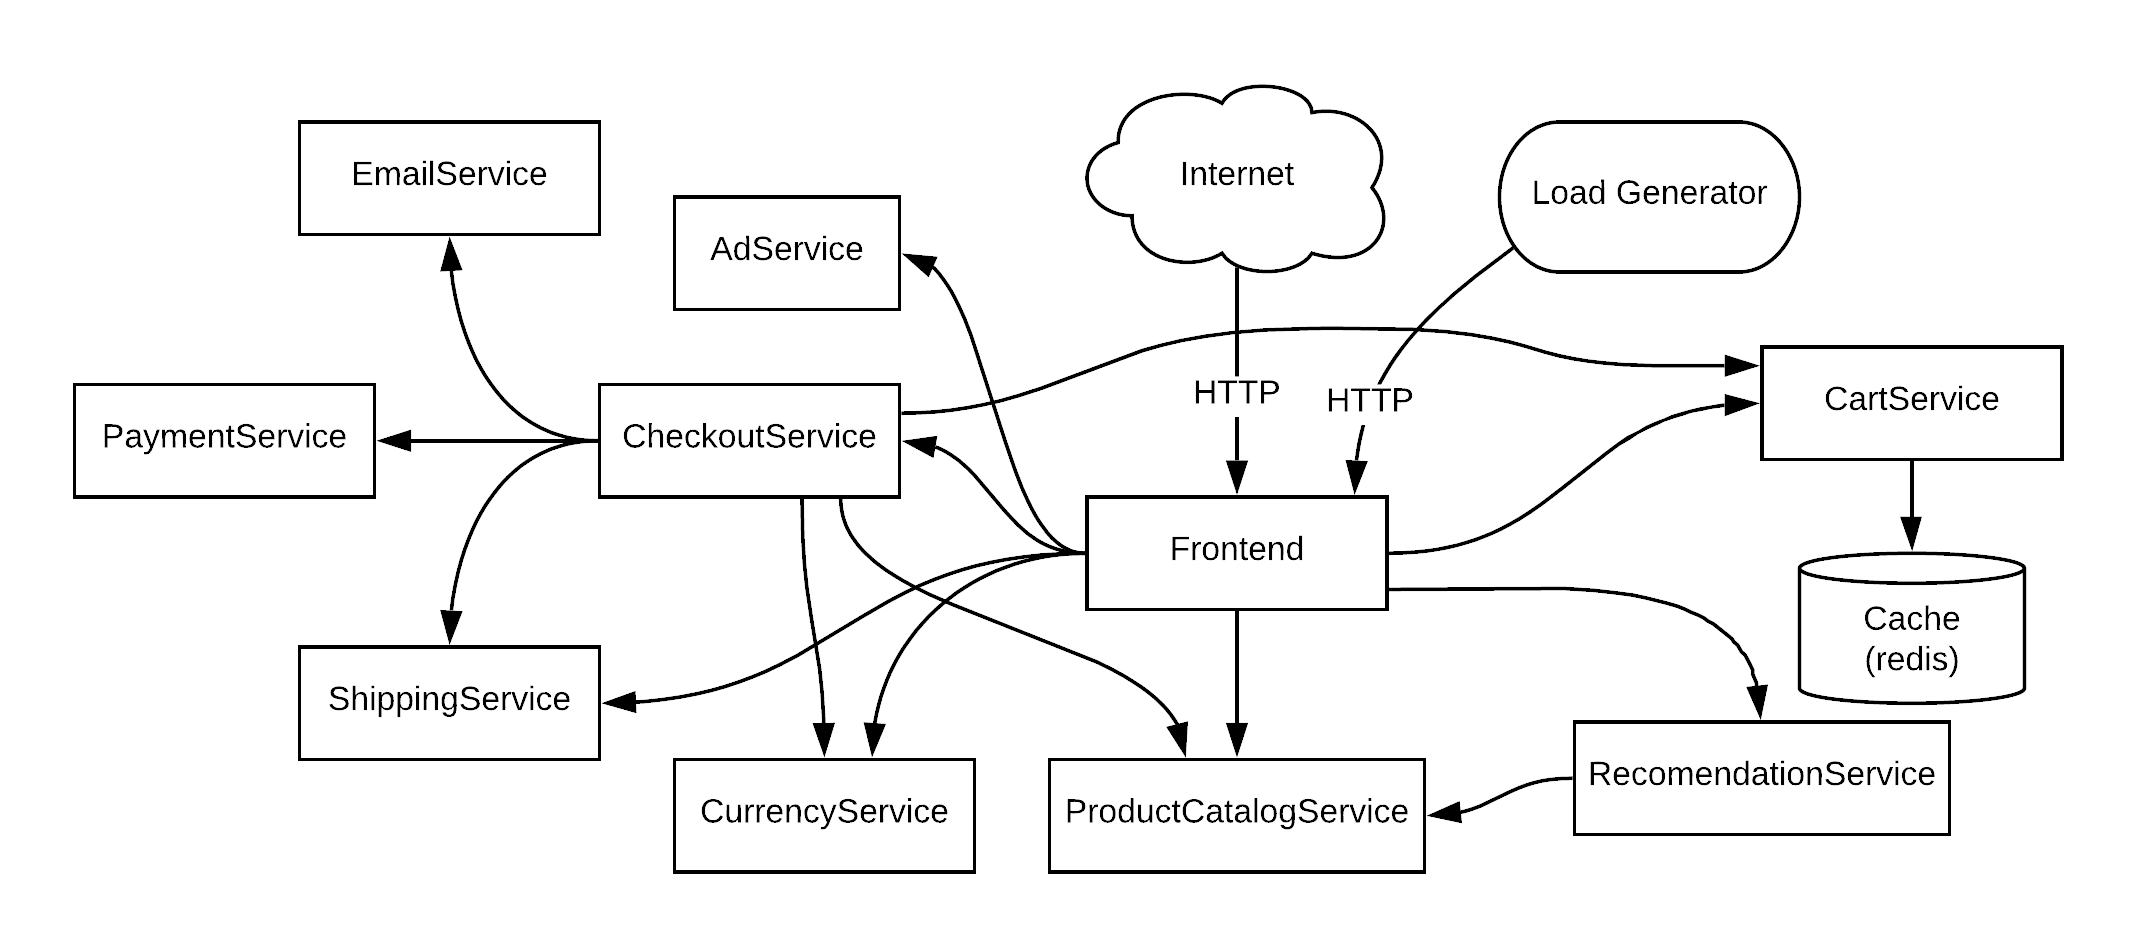
\includegraphics[width=1\textwidth]{myImages/R2.png}
\caption{Architectural diagram of GCP Online Boutique application, from repository under Apache 2.0 license}
\label{fig:R2_arch}
\end{figure}

\subsection{Microservices Design Patterns and Anti-Patterns in R2}
\label{subsec:R2_detection}

The presence of design patterns and anti-patterns have been listed in Table~\ref{table:R2_result}.

\begin{table}[H]
\centering 
    \begin{tabular}{ 
  | >{\centering\arraybackslash} m{16em} 
  | >{\centering\arraybackslash} m{2.2em} 
  | >{\centering\arraybackslash} m{16em} 
  | >{\centering\arraybackslash} m{2.2em} | }
    \hline
    \rowcolor{bluepoli!40}
    \textbf{Design Pattern} & \cmark \textbackslash – & \textbf{Anti-Pattern} & \cmark \textbackslash – \T\B \\
    \hline \hline
    API Gateway & \cmark & Wrong Cut & – \T\B\\
    \hline
    \rowcolor{bluepoli!10}
    Service Mesh with Sidecar & \cmark & Nano Microservice & – \T\B \\
    \hline
    Service Registry \& Discovery & \cmark & Mega Microservice & – \T\B \\
    \hline
    \rowcolor{bluepoli!10}
    Backends for Frontends & – & ESB Usage & – \T\B \\
    \hline
    Asynchronous Messaging & – & Hardcoded Endpoints & – \T\B \\
    \hline
    \rowcolor{bluepoli!10}
    Database per Service & – & No API Gateway & – \T\B \\
    \hline
    API Composition & – & Shared Persistence & – \T\B \\
    \hline
    \rowcolor{bluepoli!10}
    CQRS & – & No CI/CD & – \T\B \\
    \hline
    Event Sourcing & – & Multiple Service Instances per Host & – \T\B \\
    \hline
    \rowcolor{bluepoli!10}
    Service Instance per VM & – & No API Versioning & \cmark \T\B \\
    \hline
    Service Instance per Container & \cmark & No Health Check & – \T\B \\
    \hline
    \rowcolor{bluepoli!10}
    Serverless & – & Local Logging & – \T\B \\
    \hline
    Health Check & \cmark &  & \T\B \\
    \hline
    \rowcolor{bluepoli!10}
    Distributed Tracing & \cmark & & \T\B \\
    \hline
    Log Aggregator & \cmark &  & \T\B \\
    \hline
    \rowcolor{bluepoli!10}
    Circuit Breaker & – &  & \T\B \\
    \hline
    \end{tabular}
    \\[10pt]
    \caption{Presence of microservice design patterns and anti-patterns in repository R2}
    \label{table:R2_result}
\end{table}

To clarify each pattern or anti-pattern item, a few sentences are provided below.

\paragraph{API Gateway} The "frontend" microservice serves static web app assets (HTML, CSS, JS) and acts as an API gateway by making the appropriate gRPC calls to other business domain microservices when an HTTP request is made to an endpoint, providing the clients with a single entry point to communicate with microservices.

\paragraph{Service Mesh with Sidecar} Similar to the eShopOnContainers application, the use of a service mesh is provided as an option and sidecar configuration files are given for only one microservice.
When the application is to be deployed to GCP cloud, by applying "istio-manifests.yaml" file, the "frontend" service can be injected with a sidecar and communicate with other GCP services for monitoring, profiling and other similar tasks. 
Additionaly, instructions for GCP service mesh Anthos\footnotemark[72]\footnotetext[72]{\href{https://cloud.google.com/anthos/service-mesh}{https://cloud.google.com/anthos/service-mesh}} are also provided.

\paragraph{Service Registry and Discovery} As with the previous project, the service registry and discovery tasks are delegated to Kubernetes.
The application of Kubernetes .yaml files containing Kubernetes "deployment" and "service" object descriptions per microservice container solves this critical aspect for the Online Boutique project.

\paragraph{Backends for Frontends} In this application, there is no multiple microservice implementations or detected configurations for different kinds of clients.

\paragraph{Asynchronous Messaging} The architecture does not contain a message broker such as RabbitMQ or any other temporary message storage mechanism.
Communication between microservices are done through the synchronous gRPC calls.

\paragraph{Database per Service} Out of the ten microservices, the only microservice that uses a database is the "cart" microservice, which stores and retrieves user's items in his/her shopping cart in Redis key-value store, instantiated as a separate container.
Because of the limited complexity of the application, the database per service pattern is not needed and utilized.

\paragraph{API Composition} The "frontend" microservice makes calls to multiple microservices and combines the responses into one data structure to be rendered in an HTML template as a response to specific endpoints.
Because a separate aggregator service is not present, according to the detection criteria, the API composition pattern is not utilized.

\paragraph{CQRS} The only microservices that reads and writes data is the "cart" microservice and there is no separation of read and write tasks that signals the presence of CQRS pattern.

\paragraph{Event Sourcing} The application does not make use of notion of events and does not contain an event store.

\paragraph{Service Instance per Virtual Machine} The repository does not contain VM images as deployment option.

\paragraph{Service Instance per Container} The microservices are containerized into Docker images and the Kubernetes .yaml files are provided for running the entire application.

\paragraph{Serverless} Although the application may be deployed using serverless approach by making additional effort, in the repository, no instructions about serverless deployment is provided.

\paragraph{Health Check} The health check mechanism is implemented by using Kubernetes liveness and readiness probes, configured to execute a health check utility for gRPC applications called "grpc-health-probe"\footnotemark[73]\footnotetext[73]{\href{https://github.com/grpc-ecosystem/grpc-health-probe}{https://github.com/grpc-ecosystem/grpc-health-probe}}.

\paragraph{Distributed Tracing} Except for "payment" and "cart" microservices, all other services are instrumented with either StackDriver (renamed now as Google Cloud Operations\footnotemark[74]\footnotetext[74]{\href{https://cloud.google.com/products/operations}{https://cloud.google.com/products/operations}} or Jaeger, which are OpenCensus-compatible tracing libraries.
Additionally, StackDriver library is compatible with GCP so that the tracing information can also be collected by Google Cloud Trace\footnotemark[75]\footnotetext[75]{\href{https://cloud.google.com/trace}{https://cloud.google.com/trace}}.

\paragraph{Log Aggregator} The presence of log aggregator mechanism depends on the selected deployment method.
When deployed locally using Kubernetes, the logs of all microservices can be collected and saved to a file but cannot be analyzed efficiently since the logs might not have the same structure and text readers might not have filtering mechanisms helpful for particular log reading.
On the other hand, the deployment on GCP Google Kubernetes Engine (GKE) method offers automatic structured logging and filtering options since containers are automatically injected with StackDriver logging agent when deployed on GKE.

\paragraph{Circuit Breaker} The application in its current state does not employ circuit breaker pattern but additional service mesh Istio configuration files can be created and applied to enable the tripping mechanism when deployed on Istio.

\paragraph{Wrong Cut} The architecture consists of one frontend/API gateway service, one load generator service for tinkering purposes and nine business domain microservices, namely "cart", "productcatalog", "currency", "payment", "shipping", "email", "checkout", "recommendation" and "ad" services, implemented in various programming languages, all executing logic based on their names.
As a result, the layered separation of wrong cut anti-pattern is not detected.

\paragraph{Nano or Mega Microservices} The gRPC API definitions are given "demo.proto" file, which is a gRPC file used to auto-generate client libraries according to API definitions in various languages.
From this file, it is seen that each microservice has three or four API endpoints, implying that there is not significant difference in the amount of tasks the microservices carry out.
As a side note, only the two "currency" and "frontend" microservices might be discussed as potential candidates for nano and mega microservices, respectively.
Separating the task of converting currencies and updating on the latest conversion rates as a separate business domain and a microservice might be an excessive interpretation and be an example of nano microservice, while combining the frontend and API gateway tasks in a single microservice might constitute an example of mega microservice.
Nonetheless, considering the scope of the entire application, it is safe to conclude that there is not a big difference that would be seen in microservice applications with true nano or mega microservice anti-patterns.

\paragraph{ESB Usage} The architecture does not contain any simple or advanced message broker mechanism.

\paragraph{Hardcoded Endpoints} One hardcoded IP address that is not excluded as explained in the adopted method section was "169.254.169.254", in the deployment files to be used to deploy the application on GCP cloud proud. 
However, upon further investigation it has been seen that the mentioned IP address is a private IP address, not to be used on the Internet, and used by the containers to access the metadata of the hosting VM, when deployed on cloud.
In this case, the IP address would be, when deployed on GCP, the metadata server of Google Cloud Engine (GCE), to be used to collect metadata of the VM hosting the container on cloud.
Therefore, even though the repository contains one hardcoded IP address, it is specific to one deployment scenario and is not relevant to the hardcoded endpoint anti-pattern, which is related to the absence of a service discovery mechanism.

\paragraph{No API Gateway} The architecture contains one API gateway that acts as a single entry point.

\paragraph{Shared Persistence} In the application only one microservice uses a database and the other microservices do not access the instantiated database directly, but the the API definition.
Hence, the system does not have shared persistence anti-pattern.

\paragraph{No CI/CD} The repository has GitHub Actions continuous integration files that defines unit and other tests on pushes and master releases, as a result, no CI/CD anti-pattern is avoided.

\paragraph{Multiple Service Instances per Host} Since each service is containerized into its own container, the system does not force deploying multiple services on the same host.

\paragraph{No API Versioning} The frontend microservice does not utilize API versioning on the HTTP endpoints, while other microservices does not have versioned gRPC API definitions.

\paragraph{No Health Check} The system contains health check mechanisms offered by Kubernetes, therefore does not have the related anti-pattern.

\paragraph{Local Logging} Even though the architecture does not contain a separate log collector microservice, because the cloud deployment options include log aggregator mechanism, and the microservices are supposed to be deployed to the cloud in general, it would be inappropriate to conclude that the example project contains local logging anti-pattern.
Since the microservices are instrumented with StackDriver agent to be used for cloud deployment, the system does not contain local logging anti-pattern.

\section{R3: Piggy Metrics}
\label{sec:R3}

\subsection{Overview of the Application R3}
\label{subsec:R3_overview}

The next examined repository belongs to the Piggy Metrics application, designed as a financial budget application to demonstrate Spring Boot, Spring Cloud and Docker for microservice architectures.
The three microservices "statistics service", "account service" and "notification service" constitute business domain microservices, while "auth service" deals with user authentication, each of the four services having their own MongoDB database instance.
The implementation makes use of Spring Cloud components such as API gateway Zuul\footnotemark[76]\footnotetext[77]{\href{https://github.com/Netflix/zuul}{https://github.com/Netflix/zuul}}, service discovery server Eureka, Spring Cloud support for service registry and Spring Cloud Config\footnotemark[77]\footnotetext[77]{\href{https://cloud.spring.io/spring-cloud-config/reference/html/}{https://cloud.spring.io/spring-cloud-config/reference/html/}} for centralized configuration for services.
Last but not least, the architecture contains Turbine stream aggregator\footnotemark[78]\footnotetext[78]{\href{https://github.com/Netflix/Turbine}{https://github.com/Netflix/Turbine}}, which is used to collect performance metrics from services via Spring Cloud Bus\footnotemark[79]\footnotetext[79]{\href{https://spring.io/projects/spring-cloud-bus}{https://spring.io/projects/spring-cloud-bus}} component, which in turn uses a RabbitMQ message broker instance to collect and push metrics.
The architectural diagram is shown in Figure~\ref{fig:R3_arch}, modified from the diagram in the repository in a way that reflects the current state of implementation, as the original diagram does not include ELK log aggregator mechanism and correctly shows the current state of the architecture.

\begin{figure}[H]
\centering
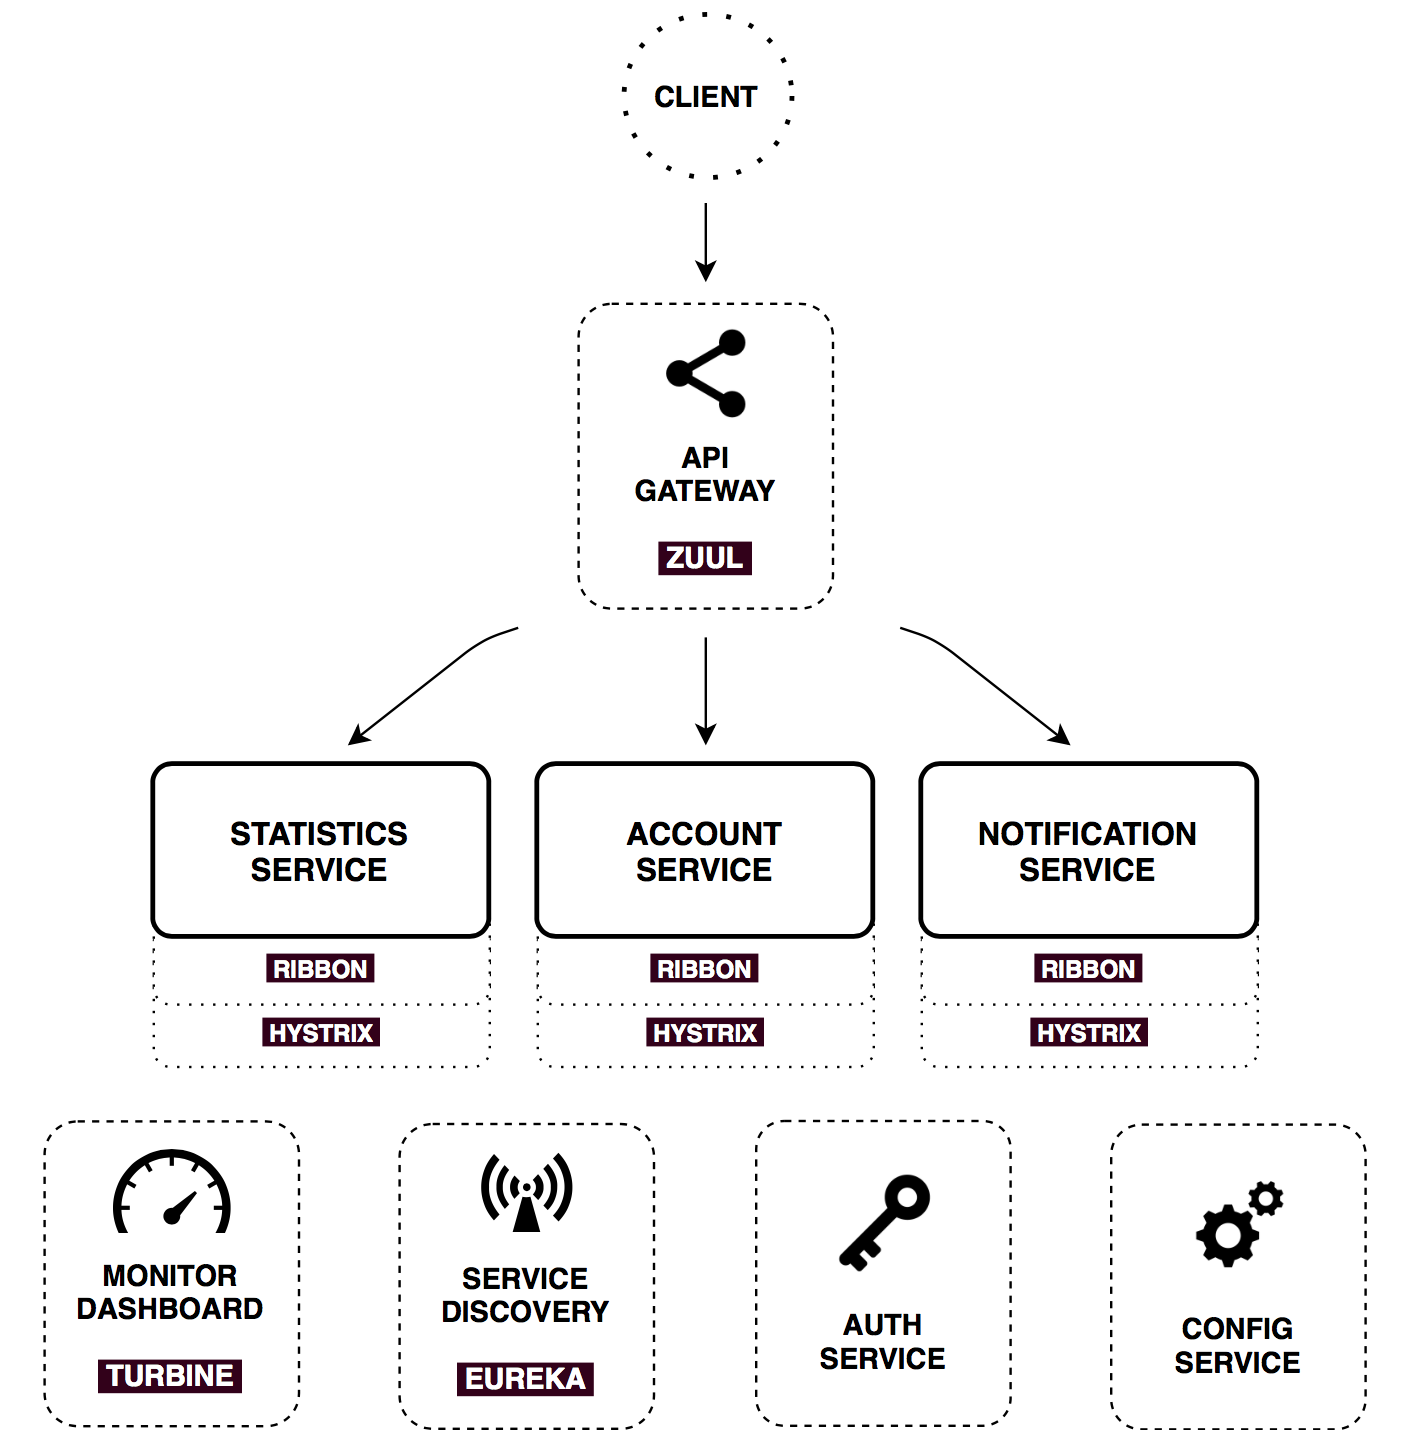
\includegraphics[width=0.9\textwidth]{myImages/R3.png}
\caption{Architectural diagram of Piggy Metrics application, adapted and modified from diagram in repository under MIT license}
\label{fig:R3_arch}
\end{figure}

\subsection{Microservices Design Patterns and Anti-Patterns in R3}
\label{subsec:R3_detection}

The presence of each pattern and anti-pattern is displayed in Table~\ref{table:R3_result}.

\begin{table}[H]
\centering 
    \begin{tabular}{ 
  | >{\centering\arraybackslash} m{16em} 
  | >{\centering\arraybackslash} m{2.2em} 
  | >{\centering\arraybackslash} m{16em} 
  | >{\centering\arraybackslash} m{2.2em} | }
    \hline
    \rowcolor{bluepoli!40}
    \textbf{Design Pattern} & \cmark \textbackslash – & \textbf{Anti-Pattern} & \cmark \textbackslash – \T\B \\
    \hline \hline
    API Gateway & \cmark & Wrong Cut & – \T\B\\
    \hline
    \rowcolor{bluepoli!10}
    Service Mesh with Sidecar & – & Nano Microservice & – \T\B \\
    \hline
    Service Registry \& Discovery & \cmark & Mega Microservice & – \T\B \\
    \hline
    \rowcolor{bluepoli!10}
    Backends for Frontends & – & ESB Usage & – \T\B \\
    \hline
    Asynchronous Messaging & – & Hardcoded Endpoints & – \T\B \\
    \hline
    \rowcolor{bluepoli!10}
    Database per Service & \cmark & No API Gateway & – \T\B \\
    \hline
    API Composition & – & Shared Persistence & – \T\B \\
    \hline
    \rowcolor{bluepoli!10}
    CQRS & – & No CI/CD & – \T\B \\
    \hline
    Event Sourcing & – & Multiple Service Instances per Host & – \T\B \\
    \hline
    \rowcolor{bluepoli!10}
    Service Instance per VM & – & No API Versioning & \cmark \T\B \\
    \hline
    Service Instance per Container & \cmark & No Health Check & – \T\B \\
    \hline
    \rowcolor{bluepoli!10}
    Serverless & – & Local Logging & \cmark \T\B \\
    \hline
    Health Check & \cmark &  & \T\B \\
    \hline
    \rowcolor{bluepoli!10}
    Distributed Tracing & \cmark & & \T\B \\
    \hline
    Log Aggregator & – &  & \T\B \\
    \hline
    \rowcolor{bluepoli!10}
    Circuit Breaker & \cmark &  & \T\B \\
    \hline
    \end{tabular}
    \\[10pt]
    \caption{Presence of microservice design patterns and anti-patterns in repository R3}
    \label{table:R3_result}
\end{table}

A few statements about each item below explains the related item concisely.

    \paragraph{API Gateway} The application is built around microservice framework Spring Cloud and the architecture contains microservice architecture components and features supported by Spring Cloud framework. 
    One such component is the Zuul API gateway component, which is implemented by Netflix and open sourced later on as part of the set of open source distributed system components, namely  Netflix OSS.
    Thanks to the support of Spring Cloud framework, Zuul API gateway is enabled by specifying the respective module in "pom.xml" and stating the "@EnableZuulProxy" annotation in a Spring application.
    The HTTP requests are automatically transmitted to underlying microservices according to the path matching routing rules defined in "gateway.yml" file, to be applied by the docker-compose file that instantiates all services.
    
    \paragraph{Service Mesh with Sidecar} The repository does not contain instruction to deploy the application on a service mesh or to inject individual microservices with a sidecar proxy.
    
    \paragraph{Service Registry and Discovery} Another Netflix OSS component supported by Spring Cloud framework is the Eureka service registry component.
    Similar to the API gateway, service registry is enabled by a dependency in "pom.xml" and a "@EnableEureka- Server" annotation in a Spring application.
    The microservices that has "@EnableDiscoveryClient" annotation are automatically registered to the Eureka service registry and microservices can look up the location of other services by the service names.
    The location of the Eureka instance is provided by Spring Cloud Config server to all microservice instances, which stores the configurations for microservices locally or points to a remote GitHub repository that stores the configurations.
    
    \paragraph{Backends for Frontends} The repository does not contain different implementations of the same business or aggregator microservice instance or different endpoints for different kinds of clients.
    
    \paragraph{Asynchronous Messaging} The business microservices only communicate with the API gateway microservice, which also serves static frontend assets to be client browser, and only communicates through synchronous HTTP requests.
    As a side note, the architecture contains one RabbitMQ instance not for conveying business domain related messages but for pushing application metrics to a monitoring service.
    Because the business microservices only use synchronous communication, the asynchronous messaging pattern is not utilized.
    
    \paragraph{Database per Service} The three business microservices "account", "notification" and "statistics" each has their own separate MongoDB instances, which is the suggested solution that offers maximum separation of tasks in terms of data storage, access and deployment.
    
    \paragraph{API Composition} The architecture does not contain any aggregator service that composes API calls to answer a complex query.
    
    \paragraph{CQRS} There is no separation of command and query aspects per microservice or handler logic basis.
    
    \paragraph{Event Sourcing} The communication mechanism does not utilize notion of messages and an event store is not present in the system.
    
    \paragraph{Service Instance per Virtual Machine} The repository does not contain VM images as a readily provided deployment option.
    
    \paragraph{Service Instance per Container} The microservices are containerized into Docker images and stored in Docker Hub to be downloaded and instantiated by applying the provided docker-compose file.
    
    \paragraph{Serverless} Similar to other projects, no instructions about serverless deployment is provided deploy the application in the repository.
    
    \paragraph{Health Check} The clients that register to the Eureka service registry periodically send heartbeat signals to the Eureka instance, in order to stay registered in the registry so that the other services can locate them.
    Additionaly, Eureka provides a dashboard in the browser that displays the status of registered microservices.
    
    \paragraph{Distributed Tracing} The distributed tracing pattern is employed through the use of another component of the Spring Cloud ecosystem.
    As with other Spring Cloud libraries, the distributed tracing library Spring Cloud Sleuth is included as a dependency inside the "pom.xml" file, and it automatically tags the logs with the labels "spanId" and "traceId".
    The architecture does not contain a compatible trace collector service, such as a Zipkin server.
    Nonetheless, because microservices are instrumented with trace generating instruments, it is concluded that the system is ready for enabling the distributed tracing mechanism.
    
    \paragraph{Log Aggregator} The application does not contain a log aggregator service.
    
    \paragraph{Circuit Breaker} The circuit breaker pattern is implemented through the use of Feign\footnotemark[80]\footnotetext[80]{\href{https://spring.io/projects/spring-cloud-openfeign}{https://spring.io/projects/spring-cloud-openfeign}} and Hystrix Spring Cloud libraries.
    Feign is a HTTP web client that makes implementing microservices easier by providing a set of tools often needed in microservice architectures, and Hystrix is, although can be used without Feign, one such tool that implements circuit breaker pattern.
    Additionaly, by adding additional annotations, Hystrix provides users with a dashboard that displays whether the communication circuit is open or closed, number of errors and average latency of remote procedure calls.
    
    \paragraph{Wrong Cut} Similar to the other inspected microservice projects, the microservices are constructed around separate business domains.
    Being a banking system that displays incomes, outcomes and savings, the application consists of "accounts", "statistics" and "notifications" microservices with additional microservices that deals with API call routing, identity, performance monitoring, configuration and service discovery.
    Because the core microservices are not layered as explained in the state-of-the-art section, the wrong cut anti-pattern is avoided.
    
    \paragraph{Nano or Mega Microservices} Considering the scope of the application, the number of HTTP endpoints of the three business microservices are similar and do not possess a difference that implies the presence of nano or mega microservices anti-patterns.
    
    \paragraph{ESB Usage} The application does not utilize a ESB component.
    
    \paragraph{Hardcoded Endpoints} The source code or configuration files do not contain a hardcoded IP address, as the architecture contains a service discovery mechanism.
    
    \paragraph{No API Gateway} The system makes use of Zuul API gateway, preventing the related no API gateway anti-pattern.
    
    \paragraph{Shared Persistence} The business microservices only access their own MongoDB instances directly, and use other REST API's when access to other kinds of data is needed.
    
    \paragraph{No CI/CD} The repository uses Travis CI\footnotemark[81]\footnotetext[81]{\href{https://travis-ci.org}{https://travis-ci.org}} to first trigger docker image builds on GitHub pushes, then triggers Codecov\footnotemark[82]\footnotetext[82]{\href{https://about.codecov.io}{https://about.codecov.io}} to carry out a code coverage test, and then deploys the new docker images automatically using continuous deployment method, or with one-click approach using continuous delivery option, depending on the configuration.
    
    \paragraph{Multiple Service Instances per Host} Similar to the most examined projects, the microservices are containerized into docker images, hence not resulting in the absolute need to deploy all instances on the same host.
    
    \paragraph{No API Versioning} The REST API endpoints do not have prefixes that implies API versioning practice.
    
    \paragraph{No Health Check} The microservices make use of heartbeats to the Eureka service to employ health check pattern.
    
    \paragraph{Local Logging} As stated earlier, the application does not involve a log aggregation mechanism, causing local logging anti-pattern to exist and make log analysis more difficult.

\section{R4: Event Sourcing \& CQRS Example}
\label{sec:R4}

\subsection{Overview of the Application R4}
\label{subsec:R4_overview}

The fourth examined application is an example application for event sourcing and CQRS patterns, implemented by Eventuate\footnotemark[83]\footnotetext[83]{\href{https://eventuate.io}{https://eventuate.io}} team to demonstrate the use of their Eventuate Tram event store, which is a database for storing events that utilizes MySQL and Kafka under the hood.
The business microservices are separated into two command and query sides.
The command-side services include "customer command-side service", "account command-side service" and "transactions command-side service", while the query-side services "customer query-side service" and "account query-side service" deal with query tasks from the client.
The business microservices and the API gateway are implemented as Spring Boot applications.
Figure~\ref{fig:R4_arch}, which is provided in the application repository, displays the architectural diagram of the application.

\begin{figure}[H]
\centering
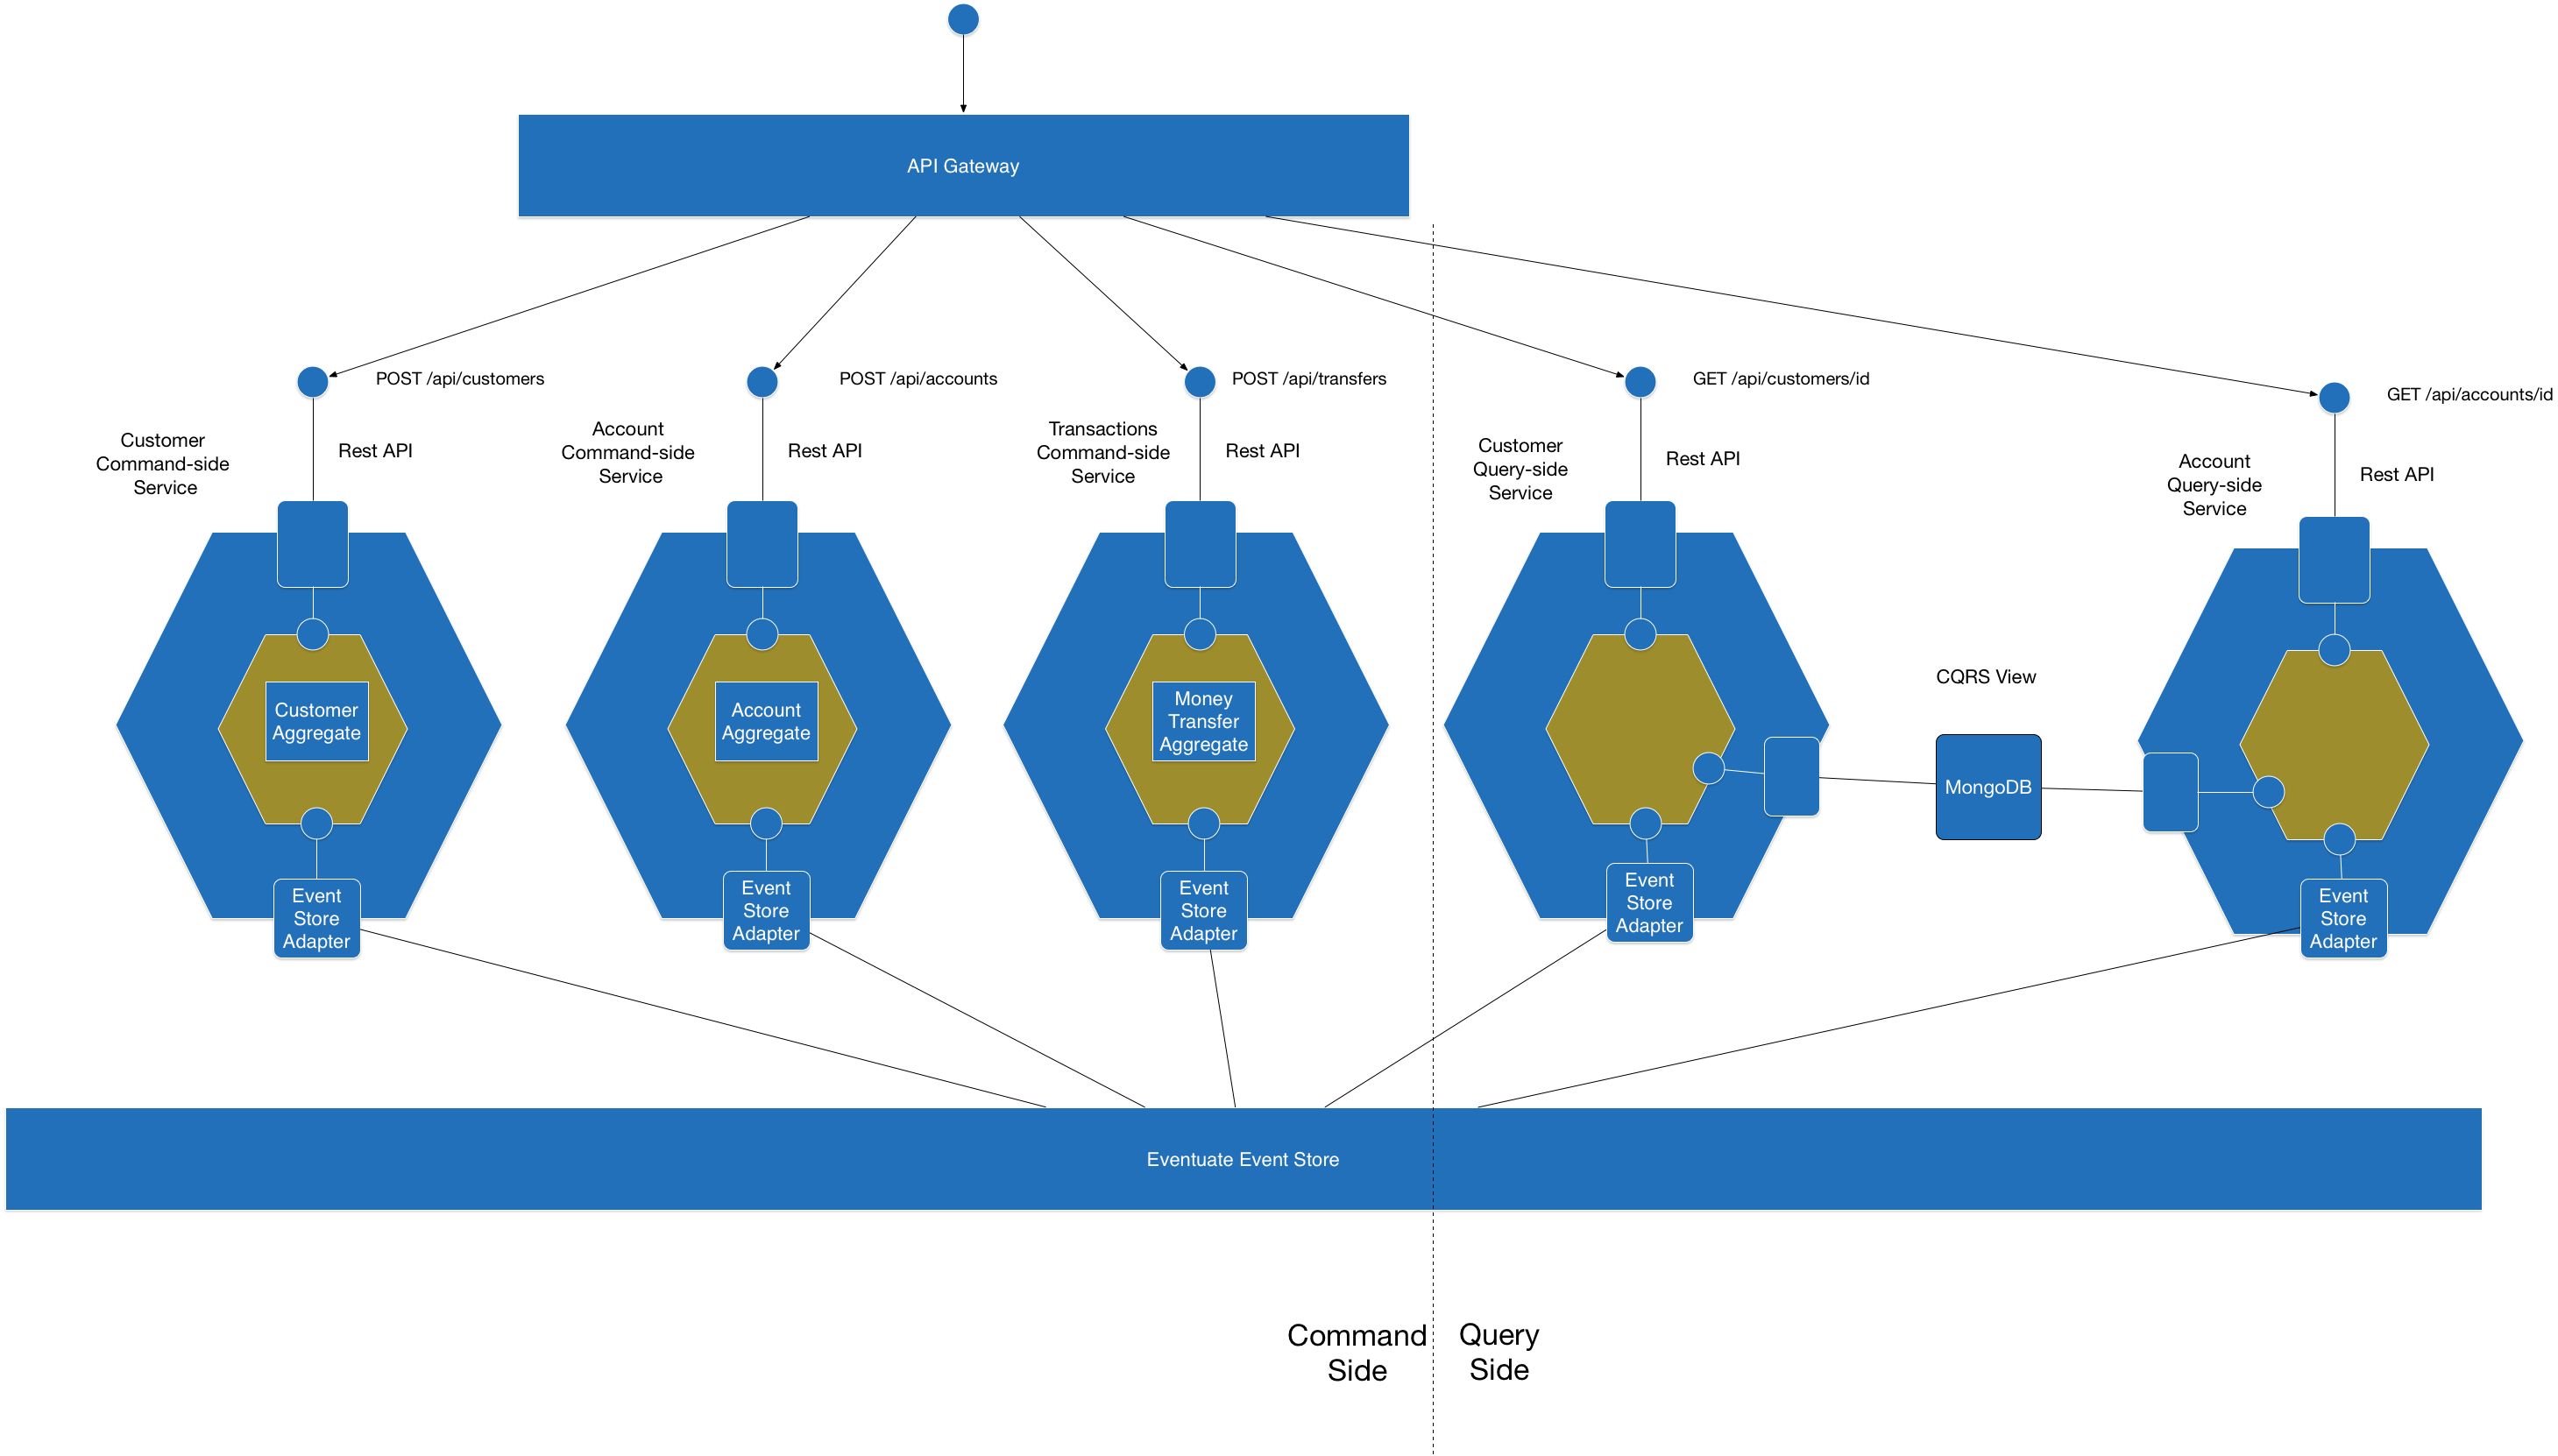
\includegraphics[width=1\textwidth]{myImages/R4.png}
\caption{Architectural diagram of Event Sourcing \& CQRS example application, by Chris Richardson under Apache 2.0 license}
\label{fig:R4_arch}
\end{figure}

\subsection{Microservices Design Patterns and Anti-Patterns in R4}
\label{subsec:R4_detection}

Table~\ref{table:R4_result} presents the presence of design patterns and anti-patterns detected in this application.

\begin{table}[H]
\centering 
    \begin{tabular}{ 
  | >{\centering\arraybackslash} m{16em} 
  | >{\centering\arraybackslash} m{2.2em} 
  | >{\centering\arraybackslash} m{16em} 
  | >{\centering\arraybackslash} m{2.2em} | }
    \hline
    \rowcolor{bluepoli!40}
    \textbf{Design Pattern} & \cmark \textbackslash – & \textbf{Anti-Pattern} & \cmark \textbackslash – \T\B \\
    \hline \hline
    API Gateway & \cmark & Wrong Cut & – \T\B\\
    \hline
    \rowcolor{bluepoli!10}
    Service Mesh with Sidecar & – & Nano Microservice & – \T\B \\
    \hline
    Service Registry \& Discovery & – & Mega Microservice & – \T\B \\
    \hline
    \rowcolor{bluepoli!10}
    Backends for Frontends & – & ESB Usage & – \T\B \\
    \hline
    Asynchronous Messaging & \cmark & Hardcoded Endpoints & \cmark \T\B \\
    \hline
    \rowcolor{bluepoli!10}
    Database per Service & – & No API Gateway & – \T\B \\
    \hline
    API Composition & – & Shared Persistence & \cmark \T\B \\
    \hline
    \rowcolor{bluepoli!10}
    CQRS & \cmark & No CI/CD & \cmark \T\B \\
    \hline
    Event Sourcing & \cmark & Multiple Service Instances per Host & – \T\B \\
    \hline
    \rowcolor{bluepoli!10}
    Service Instance per VM & – & No API Versioning & \cmark \T\B \\
    \hline
    Service Instance per Container & \cmark & No Health Check & \cmark \T\B \\
    \hline
    \rowcolor{bluepoli!10}
    Serverless & – & Local Logging & \cmark \T\B \\
    \hline
    Health Check & – &  & \T\B \\
    \hline
    \rowcolor{bluepoli!10}
    Distributed Tracing & – & & \T\B \\
    \hline
    Log Aggregator & – &  & \T\B \\
    \hline
    \rowcolor{bluepoli!10}
    Circuit Breaker & – &  & \T\B \\
    \hline
    \end{tabular}
    \\[10pt]
    \caption{Presence of microservice design patterns and anti-patterns in repository R4}
    \label{table:R4_result}
\end{table}

Next, a short clarification about each item is provided below.

\paragraph{API Gateway} The application uses a Spring Boot application implemented as a API gateway.
The routing rules are defined in a "application.properties" file based on the specifics of the HTTP request.

\paragraph{Service Mesh with Sidecar} The repository does not include instructions to deploy the application on a service mesh and the microservices are not injected with a sidecar proxy that makes the application ready for service mesh option.

\paragraph{Service Registry and Discovery} The architecture does not contain a separate service registry such as Eureka and in its current state, does not utilize a infrastructure platform such as Kubernetes.
The only deployment option readily provided is through the use of a "docker-compose" file, that is used to create a cluster (set of nodes in which containers are instantiated), and a network that is useful only in the case the cluster is created on the same physical machine.
In other words, the service discovery mechanism provided in this application in its current state only works if the entire application is deployed to the same host.
Because the application does not utilize a separate service registry and discovery mechanism or one from underlying infrastructure, the service registry and discovery pattern is not employed.

\paragraph{Backends for Frontends} The system does not have different aggregators, different implementations or endpoints of microservices depending on the kind of the client.

\paragraph{Asynchronous Messaging} The microservices employ the communication through messages and events indirectly by means of a separate event store, which is similar to a message broker but implemented also a persistent data store that stores and relays events as abstractions of data.
The pattern that captures this mechanism is called event sourcing, and since event sourcing is one way of embracing asynchronous messaging pattern, this application can be said to also have the asynchronous messaging pattern.

\paragraph{Database per Service} In this architecture the persistence tasks are delegated to the event store and individual microservice do not make use additional databases, except for two query services that create view-only schemes in MongoDB.
Because the databases do not have their own database instances, database per service pattern is not utilized.

\paragraph{API Composition} Because the system does not have aggregator or query-specific microservices, the API composition pattern is not utilized.

\paragraph{CQRS} The business domain microservices are separated into command and query microservices.
The microservices that handle the command duties include "customer command-side", "account command-side" and "transactions command-side" services, while there are "customer query-side" and "account query-side" services that execute query needs.
As the name of the project suggests, the application is designed to separate the two tasks to the full extent and create independent microservices for command and query side.
For this reason, the CQRS pattern can be said to be entirely adopted in this application.

\paragraph{Event Sourcing} As previously stated, the microservices communicate through events and delegate persistence needs to an independent event store instance.
The application uses Eventuate Local\footnotemark[84]\footnotetext[84]{\href{https://github.com/eventuate-local/eventuate-local}{https://github.com/eventuate-local/eventuate-local}} component for the event store instance, which is an open source event store built using MySQL and Kafka.
Similar to CQRS pattern, the application is built to be an example case for event sourcing pattern, specifically showcasing an open source event store and a SaaS version to be deployed on AWS, therefore employs the event sourcing pattern.

\paragraph{Service Instance per Virtual Machine} The repository does not contain readily-built VM images as a deployment option.

\paragraph{Service Instance per Container} The individual microservices are containerized into separate Docker images, making deployment using containers the go-to option for the application.

\paragraph{Serverless} In its current state, the repository does not contain instructions to deploy the application using the serverless approach.

\paragraph{Health Check} The microservices offer "/health" endpoints thanks to the Spring Boot Actuator\footnotemark[85]\footnotetext[85]{\href{https://docs.spring.io/spring-boot/docs/1.5.22.RELEASE/reference/html/production-ready-endpoints.html}{https://docs.spring.io/spring-boot/docs/1.5.22.RELEASE/reference/html/production-ready-endpoints.html}} library.
However, the architecture lacks an infrastructure or service discovery server that pings the endpoints during run-time to ensure the liveness of services or take action accordingly.
For this reason, the health check pattern is not utilized.

\paragraph{Distributed Tracing} The microservices are not instrumented with trace generating libraries and there does not exists a trace collector service.

\paragraph{Log Aggregator} Similarly, the system does not contain a log aggregation mechanism.

\paragraph{Circuit Breaker} The microservices do not make use of circuit breaker libraries offered by Spring Cloud framework and there is no infrastructure like a service mesh that readily offers the circuit breaking mechanism.

\paragraph{Wrong Cut} By separating the duties in terms of business domains and not using technical layered architecture, the wrong cut anti-pattern is preventing in this application.

\paragraph{Nano or Mega Microservices} The system consists of three command-handling "customer", "account" and "money transfer" microservices,  and two query-handling "customer" and "account" microservices, in addition to an API gateway and an event store.
Regarding the scope of the microservices, there is no difference among microservice that would result in a nano or mega microservice anti-pattern.

\paragraph{ESB Usage} The architecture does not contain an ESB for communication purposes.

\paragraph{Hardcoded Endpoints} The implementation contains hardcoded endpoints anti-pattern by specifying host addresses of all five microservices as "localhost" inside the "application.properties" file, which API gateway component uses to configure the routing of incoming requests.

\paragraph{No API Gateway} The architecture makes use of a Spring Boot application as API gateway component, hence avoiding the no API gateway anti-pattern.

\paragraph{Shared Persistence} The persistence needs of all microservices is handled by the same event store instance.
However, this design choice is related to the particular persistence mechanism selected for the application, which is using the event source pattern.
For this reason, the common use of the same event store instance is not regarded as the shared persistence anti-pattern, which usually implies using a traditional database instance for multiple microservices. 
Nonetheless, because the two query-side services make use of a single MongoDB instance in the sense that they create their own data models tailored for queries results in shared persistence anti-pattern, as the failure in the shared database instance might effect the both query services.

\paragraph{No CI/CD} The repository does not contain a CI/CD mechanism.

\paragraph{Multiple Service Instances per Host} Also with this application, the microservices are containerized, preventing the multiple service instances per host deployment anti-pattern.

\paragraph{No API Versioning} The REST endpoints do not contain any API versioning prefixes.

\paragraph{No Health Check} Although the microservices provide "/health" endpoints, no health check mechanism is implemented.

\paragraph{Local Logging} As stated in the relative pattern, the absence of log aggregation mechanism results in local logging anti-pattern in this application.

\section{R5: Food-to-Go Application}
\label{sec:R5}

\subsection{Overview of the Application R5}
\label{subsec:R5_overview}

The fifth examined application is the Food-to-Go (FTGO) application, implemented as a food ordering platform to be used by both customers and restaurants.
The application illustrates a number of microservice design patterns since it is also implemented as an example of design patterns explained in his book by software architect Chris Richardson\footnotemark[86]\footnotetext[86]{\href{https://www.chrisrichardson.net}{https://www.chrisrichardson.net}}.
The business microservices include "accounting", "consumer", "restaurant", "delivery", "order" and "order history".
For message broker purposes, Eventuate CDC (Change-Data-Capture)\footnotemark[87]\footnotetext[87]{\href{https://eventuate.io/docs/manual/eventuate-tram/latest/cdc-configuration.html}{https://eventuate.io/docs/manual/eventuate-tram/latest/cdc-configuration.html}} framework is used, which utilizes Kafka, Apache Zookeeper and MySQL under the hood.
In addition, although omitted from set of patterns to be examined in this study, saga pattern is implemented using Eventuate Tram\footnotemark[88]\footnotetext[88]{\href{https://eventuate.io/abouteventuatetram.html}{https://eventuate.io/abouteventuatetram.html}} framework for coordinating distributed business transaction across multiple microservices.
The persistence tasks of six microservices are handled by one MySQL database instance, while "order history" service uses a DynamoDB\footnotemark[89]\footnotetext[89]{\href{https://docs.aws.amazon.com/amazondynamodb/latest/developerguide/Introduction.html}{https://docs.aws.amazon.com/amazondynamodb/latest/developerguide/Introduction.html}} Local (downloadable version of DynamoDB) SQL database instance.
Last but not least, a Zipkin instance in included in the application to collect trace data from API gateway and the order service.
The architectural diagram of the application is illustrated in Figure~\ref{fig:R5_arch}.

\begin{figure}[H]
\centering
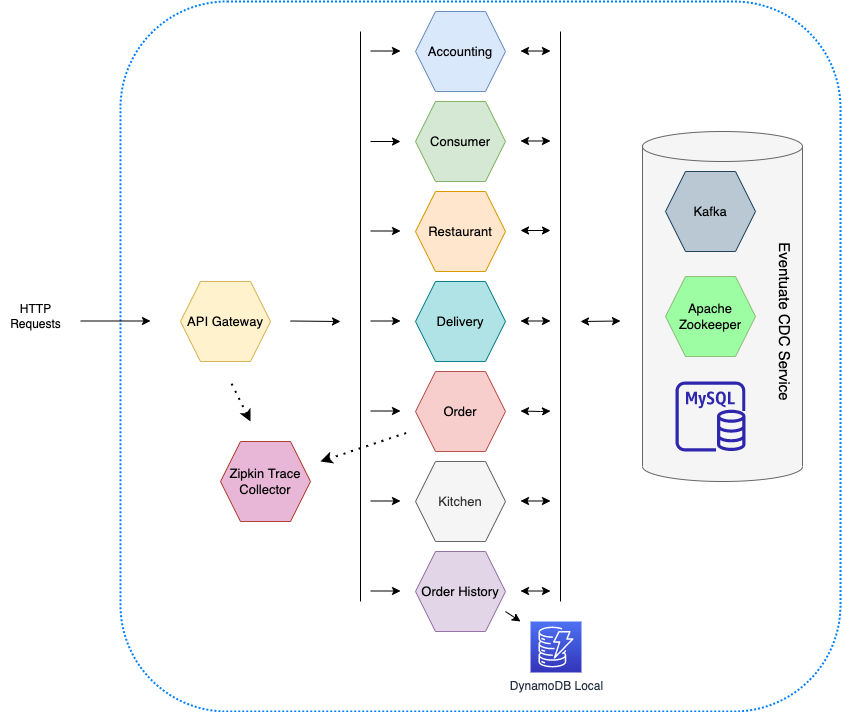
\includegraphics[width=1\textwidth]{myImages/R5.png}
\caption{Architectural diagram of Food-to-Go application}
\label{fig:R5_arch}
\end{figure}

\subsection{Microservices Design Patterns and Anti-Patterns in R5}
\label{subsec:R5_detection}

The presence of each pattern and anti-pattern is displayed in Table~\ref{table:R5_result}.

\begin{table}[H]
\centering 
    \begin{tabular}{ 
  | >{\centering\arraybackslash} m{16em} 
  | >{\centering\arraybackslash} m{2.2em} 
  | >{\centering\arraybackslash} m{16em} 
  | >{\centering\arraybackslash} m{2.2em} | }
    \hline
    \rowcolor{bluepoli!40}
    \textbf{Design Pattern} & \cmark \textbackslash – & \textbf{Anti-Pattern} & \cmark \textbackslash – \T\B \\
    \hline \hline
    API Gateway & \cmark & Wrong Cut & – \T\B\\
    \hline
    \rowcolor{bluepoli!10}
    Service Mesh with Sidecar & – & Nano Microservice & – \T\B \\
    \hline
    Service Registry \& Discovery & \cmark & Mega Microservice & – \T\B \\
    \hline
    \rowcolor{bluepoli!10}
    Backends for Frontends & – & ESB Usage & – \T\B \\
    \hline
    Asynchronous Messaging & \cmark & Hardcoded Endpoints & - \T\B \\
    \hline
    \rowcolor{bluepoli!10}
    Database per Service & – & No API Gateway & – \T\B \\
    \hline
    API Composition & – & Shared Persistence & \cmark \T\B \\
    \hline
    \rowcolor{bluepoli!10}
    CQRS & \cmark & No CI/CD & \cmark \T\B \\
    \hline
    Event Sourcing & \cmark & Multiple Service Instances per Host & – \T\B \\
    \hline
    \rowcolor{bluepoli!10}
    Service Instance per VM & – & No API Versioning & \cmark \T\B \\
    \hline
    Service Instance per Container & \cmark & No Health Check & – \T\B \\
    \hline
    \rowcolor{bluepoli!10}
    Serverless & – & Local Logging & \cmark \T\B \\
    \hline
    Health Check & \cmark &  & \T\B \\
    \hline
    \rowcolor{bluepoli!10}
    Distributed Tracing & \cmark & & \T\B \\
    \hline
    Log Aggregator & – &  & \T\B \\
    \hline
    \rowcolor{bluepoli!10}
    Circuit Breaker & – &  & \T\B \\
    \hline
    \end{tabular}
    \\[10pt]
    \caption{Presence of microservice design patterns and anti-patterns in repository R5}
    \label{table:R5_result}
\end{table}

A short comment about each design pattern and anti-pattern is provided below.

\paragraph{API Gateway} The implementation of the FTGO application uses Spring Cloud Gateway\footnotemark[90]\footnotetext[90]{\href{https://spring.io/projects/spring-cloud-gateway}{https://spring.io/projects/spring-cloud-gateway}} component as the API gateway of the application.
The routing rules are specified in the source code using the related route builder classes of Spring Cloud Gateway according to the specifics of the HTTP requests.
Additionally, for exemplary purposes, the repository contains another API gateway implemented by an API query language GraphQL\footnotemark[91]\footnotetext[91]{\href{https://graphql.org}{https://graphql.org}}, which defines APIs using types and fields, unlike REST APIs that define endpoints.

\paragraph{Service Mesh with Sidecar} The repository does not contain instructions to deploy the application on a service mesh and there is no microservices detected that has a sidecar injected.

\paragraph{Service Registry and Discovery} The application uses the service registry and discovery mechanism of Kubernetes.
Apart from this option, the architecture does not contain a service registry microservice.

\paragraph{Backends for Frontends} The application does not contain different versions of microservices, aggregators or API gateways depending on the client.

\paragraph{Asynchronous Messaging} The architecture uses Eventuate Tram framework, MySQL and Apache Kafka to implement asynchronous messaging pattern.
Eventuate Tram framework makes it easier for microservices to publish and consume domain events and commands, with the help of a compatible message broker such as Kafka for message exchange and a compatible database such as MySQL for message persistence purposes.

\paragraph{Database per Service} The application contains one DynamoDB Local instance that "order history" service uses, while the remaining six business microservices access to their own database schemas in only one MySQL instance.
According to the criteria set in this study, this is not the best practice for data persistence needs for microservices, therefore the database per service pattern is not fully utilized.

\paragraph{API Composition} The architecture does not contain separate API aggregator services although the complex business logic might involve composition of responds from multiple services.

\paragraph{CQRS} The "order history" microservice is designed to consume domain events published by other microservices and update the view-only database created in DynamoDB Local instance.
In other words, while other business microservices both handle write and read requests from client, the "order history" service does not serve any write requests directly from the user and acts as a query-only microservice.
Although the CQRS pattern is not utilized for all kinds of microservices, the "order" and "order history" microservices can be counted as an example of CQRS mechanism.

\paragraph{Event Sourcing} The event sourcing pattern is utilized in the "account" microservice, which processes events stored in the event store Eventuate Local by making use of event processing methods provided by Eventuate Client\footnotemark[92]\footnotetext[92]{\href{https://eventuate.io/docs/java/eventuate-client-framework-for-java.html}{https://eventuate.io/docs/java/eventuate-client-framework-for-java.html}} framework for Java language.

\paragraph{Service Instance per Virtual Machine} Similar to other repositories, there are no instructions or readily built VM images to deploy microservices as virtual machine images.

\paragraph{Service Instance per Container} The business microservices, API gateway and infrastructure microservices are containerized into Docker images.

\paragraph{Serverless} The repository does not contain instructions to deploy the application on a serverless platform.

\paragraph{Health Check} With the help of Spring Boot Actuator library, which implements "/health" endpoints for microservices automatically, and Kubernetes probing to the implemented health endpoints, the health check pattern is utilized.

\paragraph{Distributed Tracing} The distributed tracing pattern is implemented for exemplary purposes to show the communication only between API gateway and "order" service.
The instrumentation library used to generate traces is the Spring Cloud Sleuth\footnotemark[93]\footnotetext[93]{\href{https://spring.io/projects/spring-cloud-sleuth}{https://spring.io/projects/spring-cloud-sleuth}} library, while a Zipkin server is chosen to collect the traces and present trace data with a user interface.
Even though not all microservices are instrumented, the presence of intrumentation libraries and trace collector service shows that the distributed tracing pattern is employed to a considerable extent.

\paragraph{Log Aggregator} In the architecture there is not any log aggregator service.

\paragraph{Circuit Breaker} Similarly, there is no circuit breaker library or the use of a circuit breaking infrastructure feature that suggests the presence of circuit breaker pattern.

\paragraph{Wrong Cut} The business logic is separated into "consumer", "restaurant", "order", "kitchen", "accounting", "delivery" and "order history" microservices and not into technical layers, hence the wrong cut anti-pattern is avoided.

\paragraph{Nano or Mega Microservices} Taking into account the fact that this application is implemented as an example of a number of design patterns, the complex business logic, different communication and persistence mechanisms result in a fairly complex application.
However, noting that the nano or mega microservice anti-patterns are related to the difference in the relative share of business tasks among microservices, there is no such unequal distribution of business tasks that would suggest the presence of the mentioned anti-patterns.

\paragraph{ESB Usage} The implementation does not include an ESB component.

\paragraph{Hardcoded Endpoints} The application uses service discovery mechanism of Kubernetes and does not contain any hardcoded endpoints.

\paragraph{No API Gateway} Thanks to the use of Spring Cloud Gateway component, no API gateway anti-pattern is prevented in this application.

\paragraph{Shared Persistence} Except the "order history" service, other six microservices access to the same MySQL database instance, even though they create their own schemes.
As previously said, according to the criteria set in this study, the absence of separate database instances is count as shared persistence anti-pattern, such as in this case.

\paragraph{No CI/CD} The repository contains CircleCI\footnotemark[94]\footnotetext[94]{\href{https://circleci.com}{https://circleci.com}} configuration files as that enables continuous integration.

\paragraph{Multiple Service Instances per Host} Having separate Docker images for individual microservices prevents the absolute need to deploy all services to the same host.

\paragraph{No API Versioning} There is no API versioning detected as part of the API endpoints, resulting in the presence of this anti-pattern.

\paragraph{No Health Check} The use of Spring Boot Actuator and Kubernetes health check mechanisms prevents no health check anti-pattern.

\paragraph{Local Logging} The absence of a log aggregation mechanism results in local logging anti-pattern in this application.

\section{R6: CoolStore Microservices}
\label{sec:R6}

\subsection{Overview of the Application R6}
\label{subsec:R6_overview}

The sixth examined application is the CoolStore microservices application, which is a simple e-commerce application that is implemented to demonstrate primarily the utilization of Microsoft Tye\footnotemark[95]\footnotetext[95]{\href{https://github.com/dotnet/tye}{https://github.com/dotnet/tye}} tool and Dapr\footnotemark[96]\footnotetext[96]{\href{https://dapr.io}{https://dapr.io}} microservice run-time for microservice applications implemented using .NET framework.
The architecture consists of five business services, namely the "identity app", "inventory app", "product catalog app", "shopping app" and "sale app", with the addition of an API gateway and frontend web application.
All of the services are instrumented with Dapr sidecars, which are similar to service mesh sidecar, but help with developing microservice applications by providing service invocation, state management and such, rather than focusing on the infrastructure related tasks.
The architectural diagram of the system is shown in Figure~\ref{fig:R6_arch}, which is provided in the repository and displayed below as it is.

\begin{figure}[H]
\centering
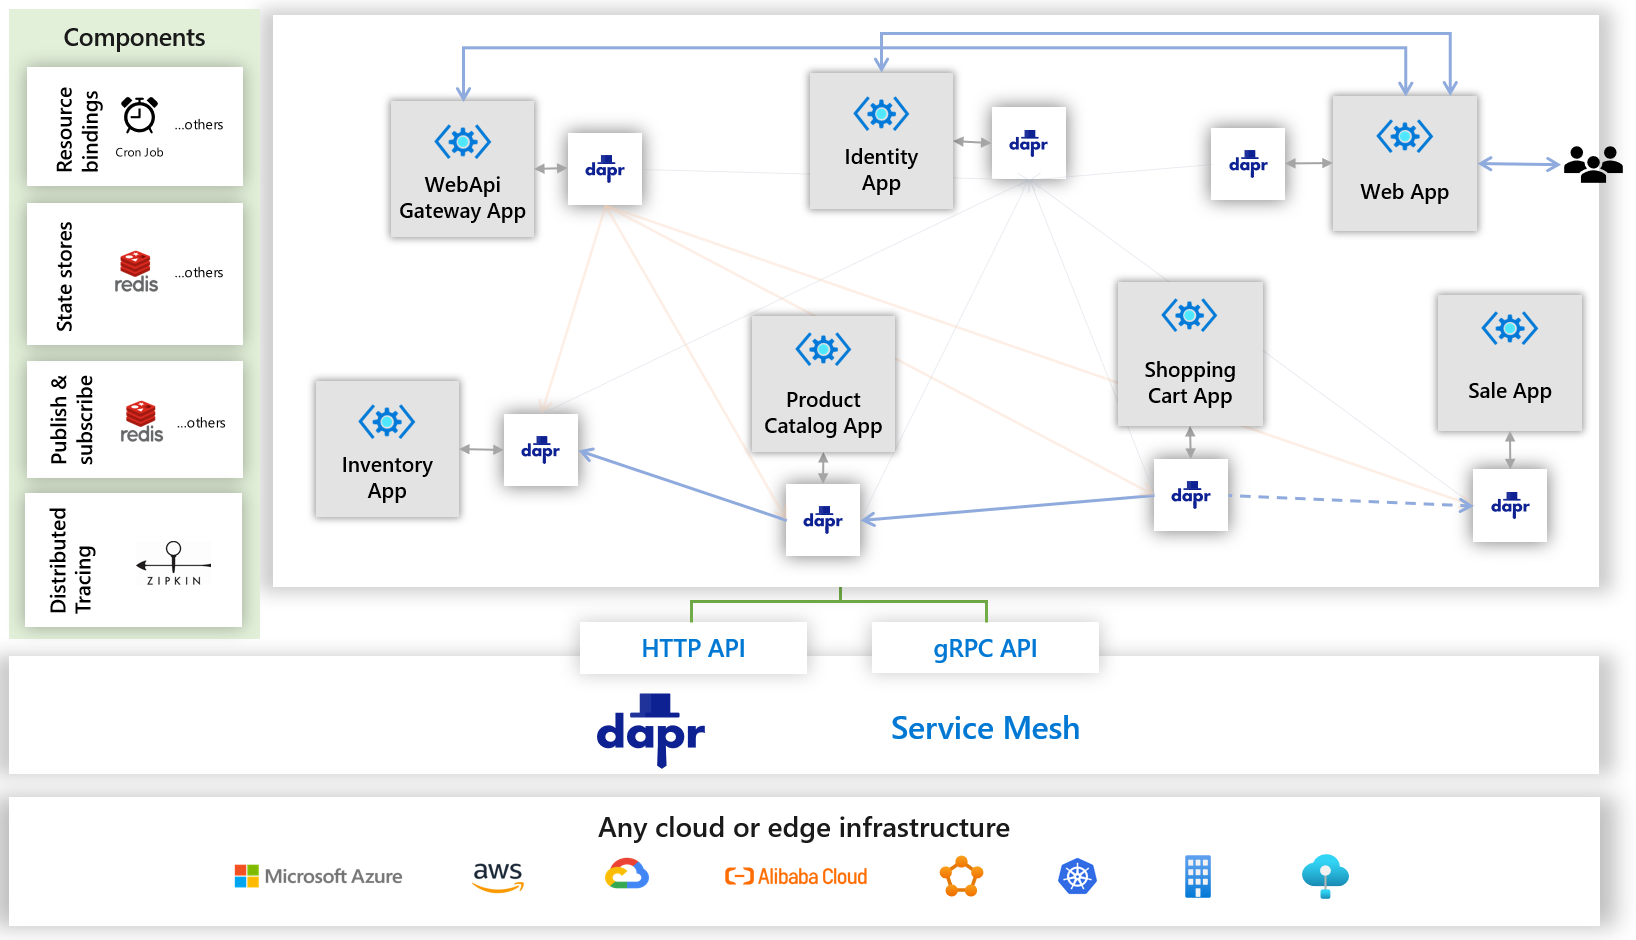
\includegraphics[width=1\textwidth]{myImages/R6.png}
\caption{Architectural diagram of CoolStore web application, by Vietnam Developer Group under MIT license}
\label{fig:R6_arch}
\end{figure}

\subsection{Microservices Design Patterns and Anti-Patterns in R6}
\label{subsec:R6_detection}

The presence of design patterns and anti-patterns are indicated in Table~\ref{table:R6_result}.

\begin{table}[H]
\centering 
    \begin{tabular}{ 
  | >{\centering\arraybackslash} m{16em} 
  | >{\centering\arraybackslash} m{2.2em} 
  | >{\centering\arraybackslash} m{16em} 
  | >{\centering\arraybackslash} m{2.2em} | }
    \hline
    \rowcolor{bluepoli!40}
    \textbf{Design Pattern} & \cmark \textbackslash – & \textbf{Anti-Pattern} & \cmark \textbackslash – \T\B \\
    \hline \hline
    API Gateway & \cmark & Wrong Cut & – \T\B\\
    \hline
    \rowcolor{bluepoli!10}
    Service Mesh with Sidecar & \cmark & Nano Microservice & – \T\B \\
    \hline
    Service Registry \& Discovery & \cmark & Mega Microservice & – \T\B \\
    \hline
    \rowcolor{bluepoli!10}
    Backends for Frontends & – & ESB Usage & – \T\B \\
    \hline
    Asynchronous Messaging & \cmark & Hardcoded Endpoints & \cmark \T\B \\
    \hline
    \rowcolor{bluepoli!10}
    Database per Service & – & No API Gateway & – \T\B \\
    \hline
    API Composition & – & Shared Persistence & \cmark \T\B \\
    \hline
    \rowcolor{bluepoli!10}
    CQRS & – & No CI/CD & – \T\B \\
    \hline
    Event Sourcing & – & Multiple Service Instances per Host & – \T\B \\
    \hline
    \rowcolor{bluepoli!10}
    Service Instance per VM & – & No API Versioning & \cmark \T\B \\
    \hline
    Service Instance per Container & \cmark & No Health Check & – \T\B \\
    \hline
    \rowcolor{bluepoli!10}
    Serverless & – & Local Logging & \cmark \T\B \\
    \hline
    Health Check & \cmark &  & \T\B \\
    \hline
    \rowcolor{bluepoli!10}
    Distributed Tracing & \cmark & & \T\B \\
    \hline
    Log Aggregator & – &  & \T\B \\
    \hline
    \rowcolor{bluepoli!10}
    Circuit Breaker & – &  & \T\B \\
    \hline
    \end{tabular}
    \\[10pt]
    \caption{Presence of microservice design patterns and anti-patterns in repository R6}
    \label{table:R6_result}
\end{table}

A short description about each item is provided below.

\paragraph{API Gateway} The architecture contains an API gateway built with .NET framework that routes incoming requests to four business domain microservices, with rules specified in the source code in "Startup.cs" file in API Gateway folder.

\paragraph{Service Mesh with Sidecar} The repository contains configuration files that injects Istio sidecars to services when the application is deployed on Azure Kubernetes Service and the service mesh Istio is installed.
Additionally, the application uses Dapr run-time, which is similar to a service mesh in injecting sidecars and controlling via a control plane, but focuses more on aiding developers with business related tasks, such as service invocation, state management and publish/subscribe mechanism\footnotemark[97]\footnotetext[97]{\href{https://docs.dapr.io/concepts/overview/}{https://docs.dapr.io/concepts/overview/}}.

\paragraph{Service Registry and Discovery} The application utilizes Tye tool, which aims to simplify microservices implementation and deployment by creating Docker files, images and pushing them to Docker Hub, generating Kubernetes files (called "manifests) and deploying applications to Kubernetes, in a way that works the same or require minimal configuration for both local and cloud deployment options\footnotemark[98]\footnotetext[98]{\href{https://github.com/dotnet/tye/blob/main/docs/reference/service_discovery.md}{Service discovery of Tye in more detail}}.
For service registry and discovery tasks, after deploying the application using "tye run" command to apply rules in "tye.yaml", Tye deploys the services on Kubernetes and uses Kubernetes service registry and discovery under the hood.
Service invocation between services is handled by combination of Dapr sidecars and Tye tool, which is enabled by specifying Dapr extension in "tye.yaml" file, which is explained more using a separate project in related directory of Tye documentation\footnotemark[99]\footnotetext[99]{\href{https://github.com/dotnet/tye/blob/main/docs/recipes/dapr.md}{https://github.com/dotnet/tye/blob/main/docs/recipes/dapr.md}}.

\paragraph{Backends for Frontends} The implementation does not contain different services or aggregators for different kinds of clients.

\paragraph{Asynchronous Messaging} The Dapr run-time provides publish/subscribe mechanism for events by making use of one of the compatible message brokers, such as Redis store in this case.

\paragraph{Database per Service} The implementation makes use of one PostgreSQL database instance, hence database per service pattern is not employed.

\paragraph{API Composition} The architecture does not contain any aggregator service.

\paragraph{CQRS} There is no division of tasks into command and query services in the project.

\paragraph{Event Sourcing} Similarly, the architecture does not involve an event store that enables event sourcing pattern.

\paragraph{Service Instance per Virtual Machine} There is no readily built VM images for this deployment pattern to be employed.

\paragraph{Service Instance per Container} The microservices are containerized into Docker images to be instantiated using Docker Compose, Kubernetes or Azure AKS.

\paragraph{Serverless} The repository does not contain instructions for serverless deployment.

\paragraph{Health Check} The application uses health check feature of .NET framework and probing function of gRPC health check utility\footnotemark[73] found in R2, specified to be executed by Kubernetes to the "/healthz" endpoints.

\paragraph{Distributed Tracing} The Dapr sidecars that run along the microservices generate trace data, while a compatible trace collector service, Zipkin server in this case, collects the traces and provides users with an interface for querying traces.

\paragraph{Log Aggregator} The architecture uses Serilog structured logger for logging events and Dapr provides ability to send the logs to a compatible log collector, such as Fluentd server or Azure OMS cloud service.
However, because the architecture does not contain a log aggregator in its current state, the log aggregator pattern is not utilized.

\paragraph{Circuit Breaker} The application does not apply circuit breaker pattern through libraries or as an enabled capability through underlying infrastructure.

\paragraph{Wrong Cut} The application is intended to be an e-commerce application and business microservices are separated into "identity", "inventory", "product catalog", "shopping cart" and "sale" microservices.
Since the application is not separated into technical layers, the wrong cut anti-pattern is avoided.

\paragraph{Nano or Mega Microservices} Regarding the division of business tasks and the fact that each service has three or four API endpoints, there is no difference in size between microservices that resembles nano or mega microservice anti-pattern.

\paragraph{ESB Usage} The architecture does not contain any ESB component.

\paragraph{Hardcoded Endpoints} The implementation contains IP addresses such as "0.0.0.0" and "127.0.0.1" as part of Helm values, however these variables are not used while replacing variables with actual values in creating Kubernetes manifests.
The application uses service discovery mechanism of Tye and Kubernetes in case the application is deployed using Tye, which does not utilize any hardcoded endpoints in this case.
In other cases where the microservices are instantiated one-by-one in the same host, the folders of each service contain "appsettings.json" files that have key-value pairs, pointing to, for example, identity service by specifying "http://localhost:5001".
Because of these cases, we could state that the implementation contains hardcoded endpoints that can be used to locate services, in case the actual service discovery mechanism by Tye and Kubernetes are not utilized in the deployment of application.

\paragraph{No API Gateway} Because of the presence of an API gateway, this anti-pattern is avoided.

\paragraph{Shared Persistence} In the "tye.yaml", which is a configuration file for Tye deployment tool, the same connection string to PostgreSQL database instance is used by "inventory", "product catalog" and "sale" microservices.
According to the detection criteria, the application hence contains shared persistence anti-pattern.

\paragraph{No CI/CD} The repository includes a Travis CI file that triggers Docker image builds and pushes new images to Docker Hub upon accepted pull requests on master branch.

\paragraph{Multiple Service Instances per Host} Thanks to containerisation of services, there is no constraint that would cause deployment of all services on the same host.

\paragraph{No API Versioning} The endpoints do no contain API version numbers.

\paragraph{No Health Check} The application implements and pings health check endpoints.

\paragraph{Local Logging} The absence of a log aggregator service results in local logging anti-pattern in this application.

\section{R7: Cinema Microservices}
\label{sec:R7}

\subsection{Overview of the Application R7}
\label{subsec:R7_overview}

The next examined application is cinema microservice application, which consists of an API gateway, business microservices "booking", "cinema catalog", "movies", "notification" and "payment", and a single MongoDB instance shared by services, without any frontend service that provides a graphical UI to users.
Unlike other examined applications in this study, the last commit on this repository has taken place in 2017, which suggests a "red flag" from a software engineering perspective since it has not been maintained for at least four years.
Indeed, the project does not makes use of modern solutions such as Kubernetes and utilizes Docker Swarm, a cluster management tool for Docker images that is different from Docker "swarm mode" and not actively maintained, as stated in an official announcement\footnotemark[100]\footnotetext[100]{\href{https://docs.docker.com/engine/swarm/}{https://docs.docker.com/engine/swarm/}}.
In addition, the implementation of the project is not quite self-explanatory and the blog post provided for explanation is outdated and not clear.
Nonetheless, even though this project is not one of the reference projects from well-known software companies or good developer teams, this project is included in this study in order to take a look at changes over the years in understanding of microservice principles and used libraries and tools.
Figure~\ref{fig:R7_arch} shows the architectural diagram of the application.

\begin{figure}[H]
\centering
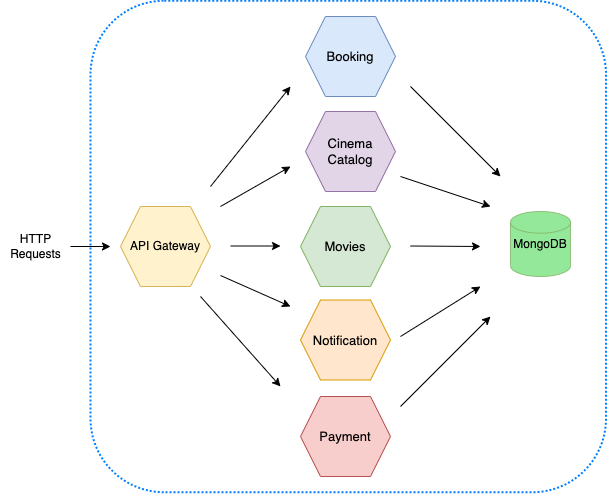
\includegraphics[width=0.8\textwidth]{myImages/R7.png}
\caption{Architectural diagram of Cinema microservices application}
\label{fig:R7_arch}
\end{figure}

\subsection{Microservices Design Patterns and Anti-Patterns in R7}
\label{subsec:R7_detection}

The presence of each design pattern and anti-pattern is provided in Table~\ref{table:R7_result}.

\begin{table}[H]
\centering 
    \begin{tabular}{ 
  | >{\centering\arraybackslash} m{16em} 
  | >{\centering\arraybackslash} m{2.2em} 
  | >{\centering\arraybackslash} m{16em} 
  | >{\centering\arraybackslash} m{2.2em} | }
    \hline
    \rowcolor{bluepoli!40}
    \textbf{Design Pattern} & \cmark \textbackslash – & \textbf{Anti-Pattern} & \cmark \textbackslash – \T\B \\
    \hline \hline
    API Gateway & \cmark & Wrong Cut & – \T\B\\
    \hline
    \rowcolor{bluepoli!10}
    Service Mesh with Sidecar & – & Nano Microservice & – \T\B \\
    \hline
    Service Registry \& Discovery & \cmark & Mega Microservice & – \T\B \\
    \hline
    \rowcolor{bluepoli!10}
    Backends for Frontends & – & ESB Usage & – \T\B \\
    \hline
    Asynchronous Messaging & – & Hardcoded Endpoints & \cmark \T\B \\
    \hline
    \rowcolor{bluepoli!10}
    Database per Service & – & No API Gateway & – \T\B \\
    \hline
    API Composition & – & Shared Persistence & \cmark \T\B \\
    \hline
    \rowcolor{bluepoli!10}
    CQRS & – & No CI/CD & \cmark \T\B \\
    \hline
    Event Sourcing & – & Multiple Service Instances per Host & – \T\B \\
    \hline
    \rowcolor{bluepoli!10}
    Service Instance per VM & – & No API Versioning & \cmark \T\B \\
    \hline
    Service Instance per Container & \cmark & No Health Check & \cmark \T\B \\
    \hline
    \rowcolor{bluepoli!10}
    Serverless & – & Local Logging & \cmark \T\B \\
    \hline
    Health Check & – &  & \T\B \\
    \hline
    \rowcolor{bluepoli!10}
    Distributed Tracing & – & & \T\B \\
    \hline
    Log Aggregator & – &  & \T\B \\
    \hline
    \rowcolor{bluepoli!10}
    Circuit Breaker & – &  & \T\B \\
    \hline
    \end{tabular}
    \\[10pt]
    \caption{Presence of microservice design patterns and anti-patterns in repository R7}
    \label{table:R7_result}
\end{table}

Furthermore, a short comment about each item has been provided below.

\paragraph{API Gateway} The application contains an API gateway implemented in Node.js that routes requests to five business microservices.
The API definitions are specified using RAML\footnotemark[101]\footnotetext[101]{\href{https://raml.org}{https://raml.org}} API definition tool in the "api.raml" files of service folders, which is consumed by API gateway for correct routing.

\paragraph{Service Mesh with Sidecar} The implementation does not contain sidecar proxies or instructions to deploy application on a service mesh.

\paragraph{Service Registry and Discovery} The architecture uses service discovery mechanism of Docker Swarm mode, which is similar to Kubernetes in providing multi-host networking and embedded DNS server.

\paragraph{Backends for Frontends} Similarly, there is no different implementations of services or aggregators depending on the kind of the client.

\paragraph{Asynchronous Messaging} The microservices do not use events and message queues but only use synchronous HTTP calls.

\paragraph{Database per Service} The application contains one MongoDB instance with two replica sets, which holds the same data for redundancy and high-availability purposes.
Because the microservices do not have their own database instances, the database per service pattern is not employed.

\paragraph{API Composition} The application does not contain a separate API composer service.

\paragraph{CQRS} The microservices are not grouped into command and query groups in this application.

\paragraph{Event Sourcing} Similarly, the system does not involve an event store.

\paragraph{Service Instance per Virtual Machine} The repository does not contain readily built VM images.

\paragraph{Service Instance per Container} The repository does not contain readily built Docker images, however the deployment scripts build one Docker image per service, hence the service instance per container pattern can be said to be employed.

\paragraph{Serverless} There is no instructions for serverless deployment in the repository.

\paragraph{Health Check} No manual or readily-provided health check mechanisms are detected in the application.

\paragraph{Distributed Tracing} Similarly, the services are not instrumented with trace generator mechanisms.

\paragraph{Log Aggregator} The architecture does not include a log aggregator service or structured log creation that can easily integrate with such a service.

\paragraph{Circuit Breaker} No circuit breaker feature is implemented or used from libraries or infrastructure services.

\paragraph{Wrong Cut} The system is intended to be movie querying and ticket purchasing system, so the implemented microservices are "movie", "cinema catalog", "booking", "payment" and "notification", with an API gateway.
Because of the absence of the technical layers related to domain separation tasks, wrong cut anti-pattern is avoided in this example application.

\paragraph{Nano or Mega Microservices} The scope of the application is quite small and each microservice handles two or three REST endpoints.
For this reason, there is no nano or mega microservice anti-pattern detected in this application.

\paragraph{ESB Usage} The implementation does not contain any ESB component.

\paragraph{Hardcoded Endpoints} The connection to Docker host and database servers are constructed using hardcoded private IP addresses "tcp://192.168.99.100:2376" and "192.168.99   .100:27017, 192.168.99.101:27017 and 192.168.99.102:27017" in the implementation and integration test code.

\paragraph{No API Gateway} The use of an API gateway prevents no API gateway pattern in this application.

\paragraph{Shared Persistence} The application contains one MongoDB instance, shared by all five business microservices, therefore constitutes an example of shared persistence anti-pattern.

\paragraph{No CI/CD} The repository does not make use of any CI/CD automation tool.

\paragraph{Multiple Service Instances per Host} Similar to other applications, containerisation of services prevent multiple service instances per host anti-pattern.

\paragraph{No API Versioning} There is no API version prefixes detected in the definition of endpoints.

\paragraph{No Health Check} The absence of a health check mechanism results in no health check anti-pattern for this application.

\paragraph{Local Logging} Similarly, the service logs are not sent to a log collector service, hence the application contains the local logging anti-pattern.


\section{R8: Dotnetcore Insurance Microservices}
\label{sec:R8}

\subsection{Overview of the Application R8}
\label{subsec:R8_overview}

The eight examined project is a simplified insurance sales application implemented by Altkom Software\footnotemark[102]\footnotetext[102]{\href{https://github.com/asc-lab}{https://github.com/asc-lab}} using .NET framework and compatible microservice components.
The system consists of "document", "dashboard", "product", "pricing", "payment", "policy" and "policy search" business services, with additional "chat" and "auth" services, a Vue.js frontend app, an API gateway for routing, a RabbitMQ instance for message broker purposes.
For persistence tasks, one single PostgreSQL instance is utilized for all services.
The architectural diagram is shown in Figure~\ref{fig:R8_arch}, which is provided in the related repository of the application.

\begin{figure}[H]
\centering
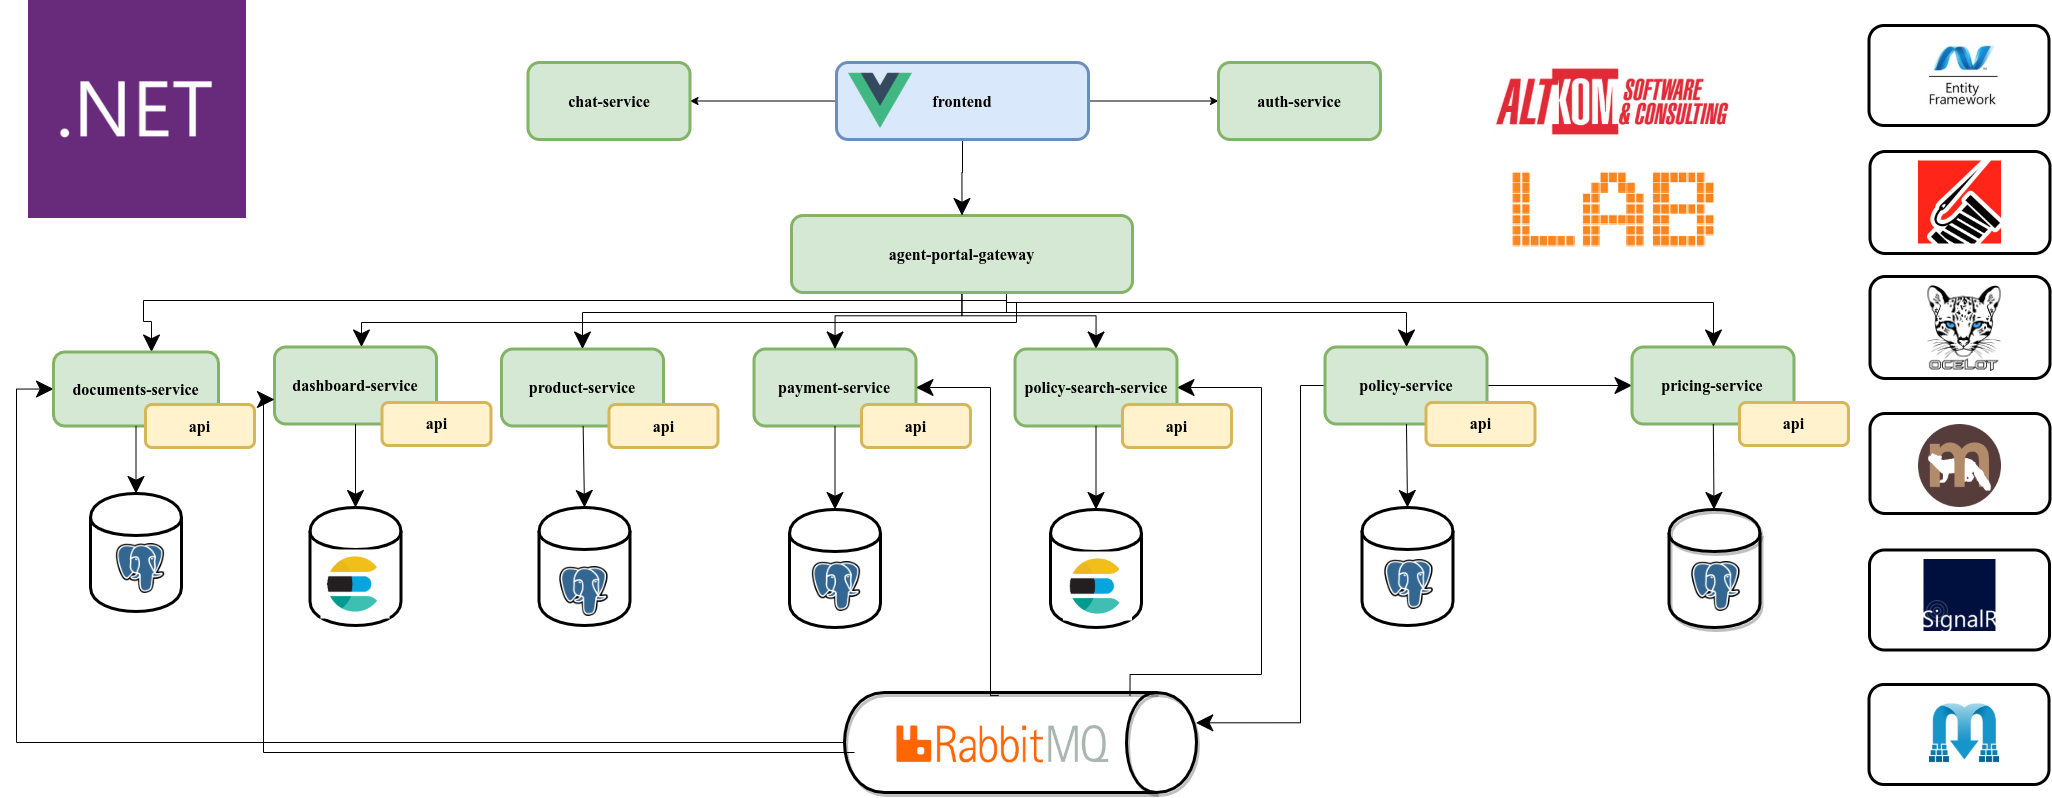
\includegraphics[width=1\textwidth]{myImages/R8.png}
\caption{Architectural diagram of Dotnetcore insurance application, by Altkom Software under Apache 2.0 license}
\label{fig:R8_arch}
\end{figure}

\subsection{Microservices Design Patterns and Anti-Patterns in R8}
\label{subsec:R8_detection}

The presence of each design pattern and anti-pattern is presented in Table~\ref{table:R8_result}.

\begin{table}[H]
\centering 
    \begin{tabular}{ 
  | >{\centering\arraybackslash} m{16em} 
  | >{\centering\arraybackslash} m{2.2em} 
  | >{\centering\arraybackslash} m{16em} 
  | >{\centering\arraybackslash} m{2.2em} | }
    \hline
    \rowcolor{bluepoli!40}
    \textbf{Design Pattern} & \cmark \textbackslash – & \textbf{Anti-Pattern} & \cmark \textbackslash – \T\B \\
    \hline \hline
    API Gateway & \cmark & Wrong Cut & – \T\B\\
    \hline
    \rowcolor{bluepoli!10}
    Service Mesh with Sidecar & – & Nano Microservice & – \T\B \\
    \hline
    Service Registry \& Discovery & \cmark & Mega Microservice & – \T\B \\
    \hline
    \rowcolor{bluepoli!10}
    Backends for Frontends & – & ESB Usage & – \T\B \\
    \hline
    Asynchronous Messaging & \cmark & Hardcoded Endpoints & – \T\B \\
    \hline
    \rowcolor{bluepoli!10}
    Database per Service & – & No API Gateway & – \T\B \\
    \hline
    API Composition & – & Shared Persistence & \cmark \T\B \\
    \hline
    \rowcolor{bluepoli!10}
    CQRS & \cmark & No CI/CD & – \T\B \\
    \hline
    Event Sourcing & – & Multiple Service Instances per Host & – \T\B \\
    \hline
    \rowcolor{bluepoli!10}
    Service Instance per VM & – & No API Versioning & \cmark \T\B \\
    \hline
    Service Instance per Container & \cmark & No Health Check & \cmark \T\B \\
    \hline
    \rowcolor{bluepoli!10}
    Serverless & – & Local Logging & \cmark \T\B \\
    \hline
    Health Check & – &  & \T\B \\
    \hline
    \rowcolor{bluepoli!10}
    Distributed Tracing & – & & \T\B \\
    \hline
    Log Aggregator & – &  & \T\B \\
    \hline
    \rowcolor{bluepoli!10}
    Circuit Breaker & – &  & \T\B \\
    \hline
    \end{tabular}
    \\[10pt]
    \caption{Presence of microservice design patterns and anti-patterns in repository R8}
    \label{table:R8_result}
\end{table}

In the following pages, we provide short explanations about each microservice pattern and anti-pattern in the application.

\paragraph{API Gateway} The architecture contains an API gateway built with .NET framework and named Ocelot\footnotemark[103]\footnotetext[103]{\href{https://github.com/ThreeMammals/Ocelot}{https://github.com/ThreeMammals/Ocelot}}, which makes it easier to integrate with .NET components.
Ocelot routes incoming HTTP requests to business microservices according to the rules specified in the JSON file "ocelot.json".

\paragraph{Service Mesh with Sidecar} The repository does not contain instructions to inject sidecars or deploy the application on a service mesh.

\paragraph{Service Registry and Discovery} The application uses Eureka service discovery server and discovery clients for microservices that registers microservices to the Eureka discovery server.
For this project, Steeltoe\footnotemark[104]\footnotetext[104]{\href{https://github.com/SteeltoeOSS/Steeltoe}{https://github.com/SteeltoeOSS/Steeltoe}} discovery client is used on microservices, which is a .NET discovery client implementation that is compatible with Eureka discovery server.

\paragraph{Backends for Frontends} There is no custom aggregators or microservices implemented regarding the particular kind of the client.

\paragraph{Asynchronous Messaging} The implementation contains a RabbitMQ message broker instance that relays business domain events between microservices.

\paragraph{Database per Service} The architecture contains one PostgreSQL database instance which is accessed by multiple business microservices, therefore does not qualify for the actual database per service pattern in this application.

\paragraph{API Composition} There is no API composer microservice found in this project.

\paragraph{CQRS} Similar to the examined project R2, the segregation of command and query tasks is implemented not on the entire application level but inside microservices with different handlers for the two tasks, by making use of MediatR library, which helps implement CQRS pattern in .NET microservices.
For example, the "policy" service separates "create policy" command from "get policy details" query, by utilizing different data models required for these two tasks.
Similarly, the "product" service separates commands that creates new products or changes the state of the products, from queries that return product details by product ID.
Additionally, there are also services that utilizes only the command or query related tasks.
For example, the "dashboard" service only conducts queries that returns information about sales of the staff, while "pricing" service only executes price calculation commands based on a number of parameters.

\paragraph{Event Sourcing} In this architecture there is no event store used to implement event sourcing pattern.
As a side note, the microservices use MartenDB\footnotemark[105]\footnotetext[105]{\href{https://github.com/JasperFx/marten}{https://github.com/JasperFx/marten}} tool, which is similar to an ORM in making it easier to talk to database entities by making use of classes, but also offers features such as enabling PostgreSQL databases to be used as a document database or an event store.
However, in this application, MartenDB is not used as an event store but as an intermediary for PostgreSQL by microservices.

\paragraph{Service Instance per Virtual Machine} There is no readily built VM images or necessary instructions in the repository.

\paragraph{Service Instance per Container} The business and infrastructure microservices are containerized in this application and can be instantiated by applying .yml files by Docker Compose.

\paragraph{Serverless} The repository does not contain instructions for serverless deployment.

\paragraph{Health Check} No manual or built-in health check mechanism is found in the application.

\paragraph{Distributed Tracing} The microservices are not instrumented and the architecture does not contain a trace collector service.

\paragraph{Log Aggregator} Although the "policy" and "pricing" services use Serilog that can be used with a log aggregator, the architecture does not contain a log aggregator service.

\paragraph{Circuit Breaker} The "policy" microservice, by making use of Polly\footnotemark[106]\footnotetext[106]{\href{https://github.com/App-vNext/Polly}{https://github.com/App-vNext/Polly}} circuit breaker library for .NET services, implements a simple retry logic in the "PricingClient.cs" file.
In case an "HttpRequestException" occurs, the policy service is configured to retry up to three times the request.
However, because the full circuit breaker feature is not used in this service or any other service, the circuit breaker pattern is not utilized in this application.

\paragraph{Wrong Cut} The application is intended to be a portal for insurance policy salespeople, hence the designed microservices are "document", "dashboard", "product", "pricing", "payment", "policy" and "policy search" services.
Because the system is divided regarding business domains and not technical layers, the wrong cut anti-pattern is prevented in this application.

\paragraph{Nano or Mega Microservices} Regarding the scope of the application, there is no imbalance detected about the amount of tasks dedicated to each service that would result in a nano or mega microservice anti-pattern.

\paragraph{ESB Usage} The architecture does not contain a ESB component for communication purposes.

\paragraph{Hardcoded Endpoints} Although the microservices have a number of "launchSettings.json" files that points to "localhost" and specific port numbers, those files are intended to be used only in development stage by .NET tools (such as Visual Studio Code or dotnet-cli) and the setting files used in containerized deployment using Docker does not contain hardcoded endpoints to specific microservices.

\paragraph{No API Gateway} The application uses Ocelot API gateway which prevents no API gateway anti-pattern.

\paragraph{Shared Persistence} The business microservices access the same single PostgreSQL instance, hence become an example of shared persistence anti-pattern in this study.

\paragraph{No CI/CD} The repository makes use of Travis CI to instantiate database and run tests upon accepted pull requests.

\paragraph{Multiple Service Instances per Host} Thanks to containerization of services, there is no absolute need to deploy multiple services to the same host.

\paragraph{No API Versioning;} The application does not utilize API versioning to define API's of microservices in a versioned manner.

\paragraph{No Health Check} The implementation is an example of no health check anti-pattern since no health mechanism is detected in the application.

\paragraph{Local Logging} Likewise, the implementation becomes an example of local logging since the architecture lacks a log aggregator service.

\section{R9: Elgris Microservice To-Do App Example}
\label{sec:R9}

\subsection{Overview of the Application R9}
\label{subsec:R9_overview}

The next examined application is an example to-do app, implemented by individual contributors, for exemplary purposes for microservices architecture.
Similar to R7, the project is not actively maintained since 2018, yet it uses Docker Compose and Kubernetes, making it easier for inspection since it provides more modern organization of services.
The systems contains a frontend service implemented in Vue.js and also takes on routing tasks as an API gateway.
The business services include "Auth API" service in Go, "Users API" in Spring Boot, "TODOs API" in Node.js and "log message processor" in Python, with a Redis instance used only between "TODOs API and "log message processor".
Last but not least, the system includes a Zipkin server instance that collect traces to construct distributed tracing data.
The architectural diagram of the application is illustrated in Figure~\ref{fig:R9_arch}, adapted from the application repository.

\begin{figure}[H]
\centering
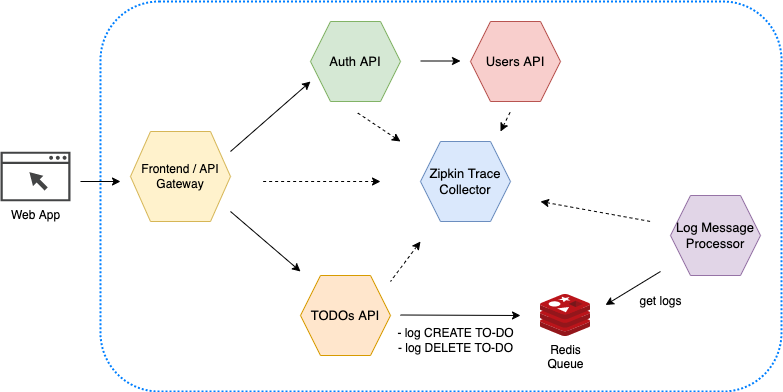
\includegraphics[width=0.95\textwidth]{myImages/R9.png}
\caption{Architectural Diagram of Example To-Do Application}
\label{fig:R9_arch}
\end{figure}

\subsection{Microservices Design Patterns and Anti-Patterns in R9}
\label{subsec:R9_detection}

The presence of design patterns and anti-patterns are indicated in Table~\ref{table:R9_result}.

\begin{table}[H]
\centering 
    \begin{tabular}{ 
  | >{\centering\arraybackslash} m{16em} 
  | >{\centering\arraybackslash} m{2.2em} 
  | >{\centering\arraybackslash} m{16em} 
  | >{\centering\arraybackslash} m{2.2em} | }
    \hline
    \rowcolor{bluepoli!40}
    \textbf{Design Pattern} & \cmark \textbackslash – & \textbf{Anti-Pattern} & \cmark \textbackslash – \T\B \\
    \hline \hline
    API Gateway & \cmark & Wrong Cut & – \T\B\\
    \hline
    \rowcolor{bluepoli!10}
    Service Mesh with Sidecar & – & Nano Microservice & – \T\B \\
    \hline
    Service Registry \& Discovery & \cmark & Mega Microservice & – \T\B \\
    \hline
    \rowcolor{bluepoli!10}
    Backends for Frontends & – & ESB Usage & – \T\B \\
    \hline
    Asynchronous Messaging & \cmark & Hardcoded Endpoints & \cmark \T\B \\
    \hline
    \rowcolor{bluepoli!10}
    Database per Service & – & No API Gateway & – \T\B \\
    \hline
    API Composition & – & Shared Persistence & – \T\B \\
    \hline
    \rowcolor{bluepoli!10}
    CQRS & – & No CI/CD & \cmark \T\B \\
    \hline
    Event Sourcing & – & Multiple Service Instances per Host & – \T\B \\
    \hline
    \rowcolor{bluepoli!10}
    Service Instance per VM & – & No API Versioning & \cmark \T\B \\
    \hline
    Service Instance per Container & \cmark & No Health Check & \cmark \T\B \\
    \hline
    \rowcolor{bluepoli!10}
    Serverless & – & Local Logging & \cmark \T\B \\
    \hline
    Health Check & – &  & \T\B \\
    \hline
    \rowcolor{bluepoli!10}
    Distributed Tracing & \cmark & & \T\B \\
    \hline
    Log Aggregator & – &  & \T\B \\
    \hline
    \rowcolor{bluepoli!10}
    Circuit Breaker & – &  & \T\B \\
    \hline
    \end{tabular}
    \\[10pt]
    \caption{Presence of microservice design patterns and anti-patterns in repository R9}
    \label{table:R9_result}
\end{table}

Next, we provide a short explanation about each pattern and anti-pattern below.

\paragraph{API Gateway} The architecture contains a frontend service component written in Vue.js that also acts as an API gateway by routing requests to "auth" and "to-do" services.

\paragraph{Service Mesh with Sidecar} The microservices do not use sidecar proxies and there is no instruction provided to deploy the application on a service mesh.

\paragraph{Service Registry and Discovery} The service registry and discovery tasks are delegated to Kubernetes by defining the "deployment" and "service" Kubernetes objects per microservice basis.

\paragraph{Backends for Frontends} In terms of responses to requests, there is no differentiation based on the kind of the requesting client.

\paragraph{Asynchronous Messaging} The architecture contains a Redis instance for demonstrating message queuing mechanism in a microservice application.
Basically, it acts as a message buffer between "to-do" and "log message processor" services.

\paragraph{Database per Service} None of the microservices in this example use a database for persistence purposes.

\paragraph{API Composition} The architecture does not contain a microservice that is implemented solely for composing API's of different services.

\paragraph{CQRS} There is no separation of the two tasks in microservice or handler level in this application.

\paragraph{Event Sourcing} The application does not use notion of events and does not contain an event store.

\paragraph{Service Instance per Virtual Machine} The microservices are not built into VM images in this repository.

\paragraph{Service Instance per Container} Similar to other examples, the microservices are built into Docker images to be instantiated by Docker Compose, Kubernetes or any other appropriate tool.

\paragraph{Serverless} The repository does not contain instructions for serverless deployment pattern.

\paragraph{Health Check} There is no manual or automatically featured health endpoint in services and no probing mechanism defined in Kubernetes .yaml files.

\paragraph{Distributed Tracing} All of the microservices are instrumented with Zipkin trace generator libraries in the programming languages they are written, and the architecture contains a Zipkin trace collector server that collects generated traces to display trace data in its UI.

\paragraph{Log Aggregator} Although one microservice is named as "message log processor", it only prints a subset of log messages generated by one single "to-do" microservice.
Because the microservices lack structured log generation and an appropriate log collector, this example application does not utilize log aggregator pattern.

\paragraph{Circuit Breaker} No circuit breaker mechanism code or library is detected in this application.

\paragraph{Wrong Cut} The application is intended as a To-Do creator with simple authentication mechanism.
Accordingly, the designed microservices are "frontend", "auth", "users", "to-do" and "message log processor", with an additional Redis instance used as message queue.
Although there are only two actual business microservices, namely "users" and "to-do", and the remaining microservices are either microservice architecture components such as "frontend" and "message queue" or cross-cutting services such as "auth", in our interpretation, it would be incorrect to conclude that the application contains the wrong cut anti-pattern, since the small scope of the application resulted in a few business microservices and the architecture is not layered into three main UI, logic and persistence layers seen in microservice applications that have the wrong cut anti-pattern.

\paragraph{Nano or Mega Microservice} Similarly,the "message log processor" would be a candidate for nano microservice anti-pattern in a regular microservice application, however, the small scope of this example makes it incorrect, in our interpretation, to conclude that the example contains a nano microservice anti-pattern.

\paragraph{ESB Usage} The architecture does not contain a ESB component.

\paragraph{Hardcoded Endpoints} Although the application uses service registry and discovery mechanism of Kubernetes, the source code contains the hardcoded IP addresses followed by the port number, such as "http://127.0.0.1:8081" in "index.js" file of frontend to point to the "auth" service, in case Kubernetes is used not for deployment and all microservices are deployed to the same host.
Because the address "127.0.0.1" is used to point to another service in the source code, this case constitutes as an example of hardocded endpoints anti-pattern.

\paragraph{No API Gateway} The presence of frontend service that acts like an API gateway prevents no API gateway anti-pattern by serving a single entry point to the microservices.

\paragraph{Shared Persistence} Because of the lack of any persistence mechanism, the shared persistence anti-pattern is not detected in this application.

\paragraph{No CI/CD} The repository does not use any CI/CD tool for automation purposes.

\paragraph{Multiple Service Instance per Host} There is no absolute need for multiple service instance per host anti-pattern to occur in this application, thanks to individual containerization of microservices.

\paragraph{No API Versioning} The endpoints of services do not utilize API versioning, hence causing this application to be an example of no API versioning anti-pattern.

\paragraph{No Health Check} The lack of health check mechanisms results in no health check anti-pattern in this implementation.

\paragraph{Local Logging} Similarly, this application becomes an example of local logging anti-pattern as a result of not utilizing a log aggregator service.

\section{R10: Run-Asp.NetCore-Microservices}
\label{sec:R10}

\subsection{Overview of the Application R10}
\label{subsec:R10_overview}

The last examined application is the Run-Asp.NetCore-Microservices application, which is an e-commerce application that has microservice architecture and implemented using .NET microservice components.
The architecture contains an API gateway, an aggregator service that serves additional API endpoints by combining calls from actual business microservices, four business microservices that have their own database instances, a RabbitMQ message broker instance and a web status service.
All four business microservices have API endpoints defined using regular HTTP, while "discount" microservice has an additional API definition using gRPC protocol.
The architectural diagram of the application is illustrated in Figure~\ref{fig:R10_arch}, which is found in the repository and displayed here as it is.

\begin{figure}[H]
\centering
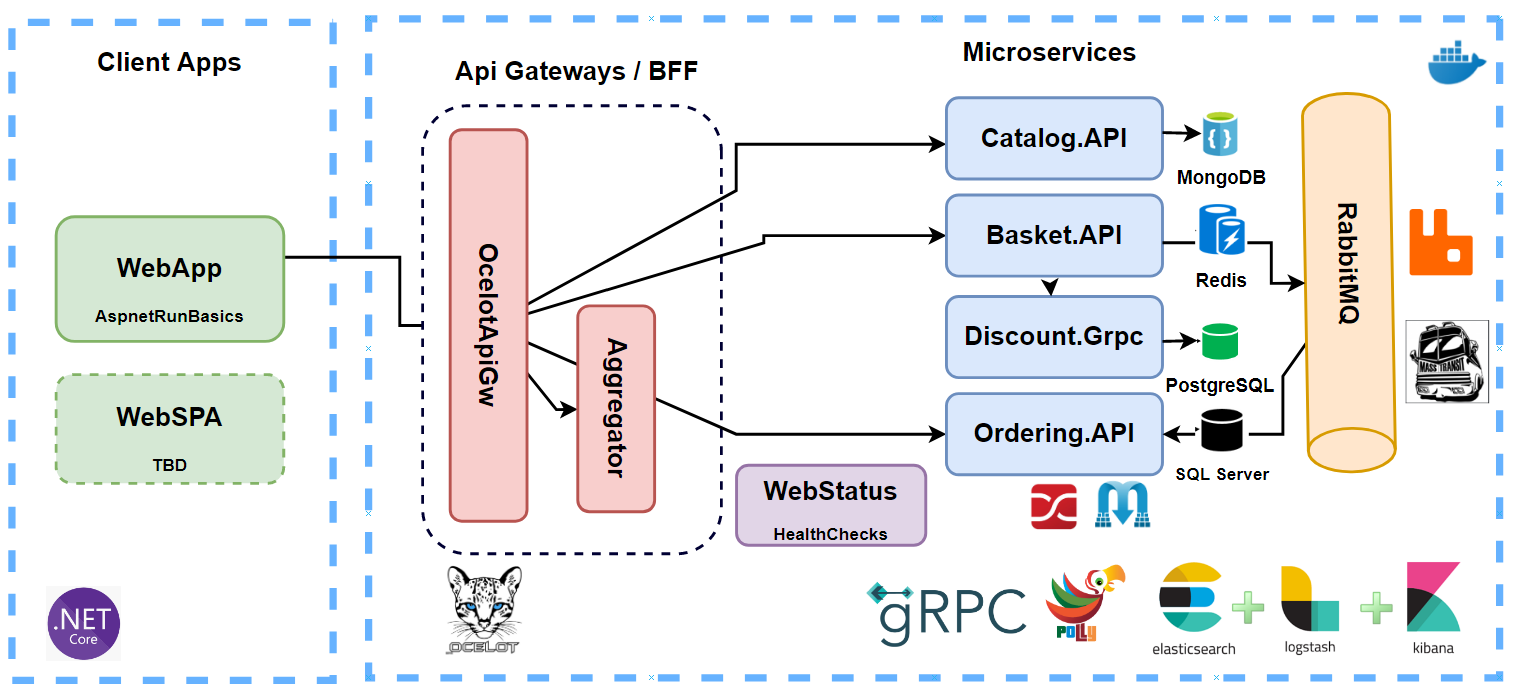
\includegraphics[width=0.95\textwidth]{myImages/R10.png}
\caption{Architectural diagram of Run-Asp.NetCore-Microservices application, by Aspnetrun under MIT license}
\label{fig:R10_arch}
\end{figure}

\subsection{Microservices Design Patterns and Anti-Patterns in R10}
\label{subsec:R10_detection}

The presence of each design pattern and anti-pattern is indicated in Table~\ref{table:R10_result}.

\begin{table}[H]
\centering 
    \begin{tabular}{ 
  | >{\centering\arraybackslash} m{16em} 
  | >{\centering\arraybackslash} m{2.2em} 
  | >{\centering\arraybackslash} m{16em} 
  | >{\centering\arraybackslash} m{2.2em} | }
    \hline
    \rowcolor{bluepoli!40}
    \textbf{Design Pattern} & \cmark \textbackslash – & \textbf{Anti-Pattern} & \cmark \textbackslash – \T\B \\
    \hline \hline
    API Gateway & \cmark & Wrong Cut & – \T\B\\
    \hline
    \rowcolor{bluepoli!10}
    Service Mesh with Sidecar & – & Nano Microservice & – \T\B \\
    \hline
    Service Registry \& Discovery & – & Mega Microservice & – \T\B \\
    \hline
    \rowcolor{bluepoli!10}
    Backends for Frontends & – & ESB Usage & – \T\B \\
    \hline
    Asynchronous Messaging & \cmark & Hardcoded Endpoints & \cmark \T\B \\
    \hline
    \rowcolor{bluepoli!10}
    Database per Service & \cmark & No API Gateway & – \T\B \\
    \hline
    API Composition & \cmark & Shared Persistence & – \T\B \\
    \hline
    \rowcolor{bluepoli!10}
    CQRS & \cmark & No CI/CD & \cmark \T\B \\
    \hline
    Event Sourcing & – & Multiple Service Instances per Host & – \T\B \\
    \hline
    \rowcolor{bluepoli!10}
    Service Instance per VM & – & No API Versioning & – \T\B \\
    \hline
    Service Instance per Container & \cmark & No Health Check & – \T\B \\
    \hline
    \rowcolor{bluepoli!10}
    Serverless & – & Local Logging & – \T\B \\
    \hline
    Health Check & \cmark &  & \T\B \\
    \hline
    \rowcolor{bluepoli!10}
    Distributed Tracing & – & & \T\B \\
    \hline
    Log Aggregator & \cmark &  & \T\B \\
    \hline
    \rowcolor{bluepoli!10}
    Circuit Breaker & \cmark &  & \T\B \\
    \hline
    \end{tabular}
    \\[10pt]
    \caption{Presence of microservice design patterns and anti-patterns in repository R10}
    \label{table:R10_result}
\end{table}

Below, the design patterns and anti-patterns in this application are concisely explained.

\paragraph{API Gateway} Similar to the project R8, the architecture contains Ocelot API gateway, which is a .Net microservice component that routes requests to the underlying four business microservices, according to the routing rules defined in "ocelot.json" file.

\paragraph{Service Mesh with Sidecar} The microservices are not injected with sidecars and the repository does not contain instructions for deployment on a service mesh.

\paragraph{Service Registry and Discovery} The application uses Docker, which provides service registry and discovery only on a single host in case a "network" in "docker-compose.yml" is defined.
The application does not even define a network a single host using this feature and calls services using "localhost" and port numbers.
Because the application lacks a service registry and discovery mechanism that is suitable for deployment in a actual distributed setting, the service registry and discovery pattern is not employed in this example.

\paragraph{Backends for Frontends} The architecture contains an aggregator service, which could be used for a different kind of client.
However, including the aggregator service, none of the microservices differentiate responses to the API calls based on the kind of client, and for this reason, the backends for frontends pattern is not utilized by this application.

\paragraph{Asynchronous Messaging} The two of the business microservices utilize RabbitMQ message broker instance for asynchronous communication, in a publish/subscribe manner.
Specifically, the "basket" microservice publishes "BasketCheckout" event, while the "ordering" service consumes the events put into the "BasketCheckout" event queue.

\paragraph{Database per Service} All four business microservices have their own SQL or NoSQL database instances.

\paragraph{API Composition} The "shopping" microservice is an example of an API composer microservice.
While it does not apply complex logic, it serves one endpoint by making calls to actual "catalog", "basket" and "ordering" business microservices and transforming the responses into a single data structure.

\paragraph{CQRS} Similar to examined .NET microservice applications, the CQRS pattern is implemented as an example inside one business microservice.
In this example, the "ordering" microservice separates checkout, create and delete order commands from order queries by making use of .NET CQRS library MediatR.

\paragraph{Event Sourcing} Although the implementation makes use of the notion of events for communication, the system lacks and event store for event sourcing pattern to be utilized.

\paragraph{Service Instance per Virtual Machine} The repository does not include readily built VM images or instruction to build and deploy them in an appropriate setting.

\paragraph{Service Instance per Container} The business and auxiliary microservices are containerized into individual Docker images, making service instance per container deployment pattern to be the go-to option for this application.

\paragraph{Serverless} Similar to other projects, the repository does not provide instructions to deploy the application on a serverless platform.

\paragraph{Health Check} The individual microservices implement "/hc" health check endpoints by utilizing the .NET health check endpoint feature, while a separate watchdog service named "WebStatus" pings the health check endpoints of services and display the status of services in a simple UI in the browser.

\paragraph{Distributed Tracing} The microservices are not instrumented with a trace generator client and the system is missing a trace collector service such as Zipkin.

\paragraph{Log Aggregator} The microservices make use of Serilog for structured logging in microservices, an ElasticSearch instance for log storage and filtering purposes and a Kibana instance for log visualisation.
Because the architecture contains all basic elements of log aggregation, it can be concluded that this application is indeed a good example of log aggregator pattern.

\paragraph{Circuit Breaker} The frontend service and the "shopping" aggregator utilize Polly library to implement circuit breaking mechanism.
Unlike the examined project R8, the services use not only the retry mechanism but actual circuit breaking feature of Polly library, by specifying the number of allowed exceptions and the time period the circuit stays in the open state.

\paragraph{Wrong Cut} The application is intended to be an example e-commerce website, so the designed microservices are "catalog", "basket", "ordering", "discount" and "shopping aggregator", along with an API gateway, event bus and monitoring services.
Similar to other examples, this application is not layered into three technical layers and hence does not contain the wrong cut anti-pattern.

\paragraph{Nano or Mega Microservices} None of the microservices seem to be a nano or mega microservice since each service handles a couple of ordinary GET and POST requests.

\paragraph{ESB Usage} The system does not contain an ESB component.

\paragraph{Hardcoded Endpoints} The implementation of application contains URLs such as "http://localhost:8000/hc" in "appsettings.json" file of web health status checking service to locate services to be checked, and URLs to "catalog", "basket" and "ordering" services in the "appsettings.json" file of API composer "shopping" service, such as "'CatalogUrl':'http://localhost:8000'".
In addition, locating the services from API gateway is done through specifying "localhost" as hosts of services and specifying port numbers of services in "ocelot.json" file, although they are not fully qualified hardcoded endpoints but hardcoded specifications to be consumed by API gateway to locate business microservices for routing purposes.
Because of these cases, the application contains the hardcoded endpoints anti-pattern.

\paragraph{No API Gateway} The presence of the Ocelot API gateway prohibits the no API gateway anti-pattern in this application.

\paragraph{Shared Persistence} The business microservices have their own different database instances and no shared connection string is detected in Docker Compose .yaml files.

\paragraph{No CI/CD} The repository does no contain any automation file to trigger a CI/CD mechanism.

\paragraph{Multiple Service Instances per Host} The business and auxiliary microservices are containerized into individual Docker images, preventing the requirement to deploy all instances to the same host.

\paragraph{No API Versioning} The endpoints of the microservices contain "api/v1/" prefix, even though the only version used is v1.
Although the version number does not seem to change during any stage of software development lifecycle, because the repository is intended to be an example microservice architecture and not an actual product to be deployed in production stage, the practice of API versioning can be said to be employed in this application.

\paragraph{No Health Check} The health check mechanisms explain in the related item prevents no health check anti-pattern for this application.

\paragraph{Local Logging} Lastly, the application avoids local logging anti-pattern by employing a structured logging tool and a log aggregator service.\\\\\\

\section{Discussion of Findings Related to Research Question 2}
\label{sec:discussion}

Referring back to the research questions, the reason why we conducted this study was to find answers to two research questions, which are about the taxonomy of design patterns and anti-patterns of microservices architecture and the presence of those patterns and anti-patterns in the popular open source microservice applications. 
In addition to the main work, regarding the second research question about the presence of patterns and anti-patterns, it is also beneficial, we believe, to take a look at the number of appearance of design patterns and anti-patterns in the examined projects.
Below, Table \ref{table:total_number} lists the total number of occurrence of patterns and anti-patterns detected during this study on the ten open source microservice projects.

\begin{table}[H]
\centering 
    \begin{tabular}{ 
  | >{\centering\arraybackslash} m{16em} 
  | >{\centering\arraybackslash} m{2em} 
  | >{\centering\arraybackslash} m{16em} 
  | >{\centering\arraybackslash} m{2em} | }
    \hline
    \rowcolor{bluepoli!40}
    \textbf{Design Pattern} & \textbf{\#} & \textbf{Anti-Pattern} & \textbf{\#} \T\B \\
    \hline \hline
    API Gateway & 10 & Wrong Cut & – \T\B\\
    \hline
    \rowcolor{bluepoli!10}
    Service Mesh with Sidecar & 3 & Nano Microservice & – \T\B \\
    \hline
    Service Registry \& Discovery & 8 & Mega Microservice & – \T\B \\
    \hline
    \rowcolor{bluepoli!10}
    Backends for Frontends & 1 & ESB Usage & – \T\B \\
    \hline
    Asynchronous Messaging & 7 & Hardcoded Endpoints & 5 \T\B \\
    \hline
    \rowcolor{bluepoli!10}
    Database per Service & 2 & No API Gateway & – \T\B \\
    \hline
    API Composition & 2 & Shared Persistence & 6 \T\B \\
    \hline
    \rowcolor{bluepoli!10}
    CQRS & 5 & No CI/CD & 5 \T\B \\
    \hline
    Event Sourcing & 2 & Multiple Service Instances per Host & – \T\B \\
    \hline
    \rowcolor{bluepoli!10}
    Service Instance per VM & – & No API Versioning & 8 \T\B \\
    \hline
    Service Instance per Container & 10 & No Health Check & 4 \T\B \\
    \hline
    \rowcolor{bluepoli!10}
    Serverless & – & Local Logging & 7 \T\B \\
    \hline
    Health Check & 6 &  & \T\B \\
    \hline
    \rowcolor{bluepoli!10}
    Distributed Tracing & 5 & & \T\B \\
    \hline
    Log Aggregator & 3 &  & \T\B \\
    \hline
    \rowcolor{bluepoli!10}
    Circuit Breaker & 2 &  & \T\B \\
    \hline
    \end{tabular}
    \\[10pt]
    \caption{Total number of design patterns and anti-patterns in examined projects}
    \label{table:total_number}
\end{table}

First observation about the number of occurrences is that, there are two design patterns that are employed in all of the examined projects, namely, the API gateway and service instance per container patterns.
The reason why the API gateway pattern is always utilized might be that, it is one of the design patterns that returns a substantial amount of value after a small investment, meaning that, it is relatively easier to understand and implement.
Also, when it is combined with required frontend tasks, as seen in most of the examined projects, it also serves static assets to the browser and provides a single entry point to the backend services.
For the service instance per container pattern, it reflects the "micro" aspect of microservice architectures quite well, provides developers with a deployment option that have a smaller learning curve with respect to service instance per VM and serverless options, and alleviates the burden of implementing or configuring services to the specifics of underlying operating system.
\\
The second observation that draws attention immediately is that there are a number of patterns and anti-patterns that are not detected in any of the examined projects.
About the deployment aspect, it might be stated that the service instance per VM and serverless patterns are not employed since they are relatively harder to learn and provides additional value with respect to per container pattern only in relatively specific cases.
For the multiple service instance per host anti-pattern, we have stated in detection criteria that even though microservices are containerized, there is no mechanism to prevent the malpractice of deploying all containers to the same host, so we checked if two or more of the microservices in an application are containerized into the same Docker image.
As a matter of fact, the containerisation of multiple services to the same container might be even harder than to containerize one service to one container image, since it would require finding more complex Docker base images than to find simpler base images such as "node:alpine" which contains Node.js run-time on top of a small Alpine Linux distribution, for services that need different run-times to be built, copied and run on top of the same Docker base image.
As a result, we might state that the microservices are in general containerized into individual images since it is easier to implement and provides better organization of the whole application.
\\
Coming to the architectural anti-patterns that are avoided in each examined application, we might observe that the design principles of microservice architectures are very well embraced and digested by the projects.
The microservices are designed around business capabilities in a balanced way and the principle of "smart endpoints, dumb pipes" is put into practice in those designs.
\\
Next, we see that the three design patterns, namely, service registry and discovery, asynchronous messaging and health check, are employed more frequently with respect to the remaining ones.
While service registry and discovery is a must for microservices to work in a distributed environment, we observe that through the use of health checks, the reliability aspect is also emphasized in those applications.
Together with tools such as Kubernetes and in essence the feedback loop that pings health endpoints of services and creates or deletes pods accordingly, health check mechanism increases fault-tolerance abilities of the application.
Additionally, the utilization of message queues is in alignment with the notion of fault-tolerance in the sense that, if implemented accordingly, the business microservices could consume messages sent by other services when they are up and running after they experience a run-time failure.
\\
Another observation about the numbers is that the most frequent anti-pattern has been no API versioning anti-pattern.
Even though it is quite simple to implement API versioning as code, because the examined applications are not actual microservice products that are maintained by a number of different development teams, it might be deemed not necessary by developers of examined repositories to make use of API versioning practice.
On the other hand, we see that even though the repositories are not actual software products, the developers of half of the repositories chose to utilize some sort of CI/CD mechanism to automatically build images or automatically test their code, as these practices are not about changing API definitions but to cope with recurrent tasks through automation during development stage.
\\
Considering the next two most frequent patterns, we observe that although the distributed tracing and CQRS patterns are not trivial to implement, five of the repositories utilize those patterns, at least as part of some of their microservices.
Visualization of inter-service calls and hence having some sort of "big-picture" view of business logic might be one of the biggest benefits for those projects utilizing distributed tracing across most of their services.
On the other hand, from a subjective point-of-view, the use of CQRS pattern might be a case of "over-engineering" in those projects, since the applications do not have many microservices and have relatively simple business logic to implement, which might be also doable without segregating the read and write tasks.
Therefore, CQRS pattern might be implemented for exemplary purposes and employed together with event sourcing pattern to feature a commercial CQRS framework as in Eventuate framework examples in R4 and R5, or to promote a CQRS library in as in MediatR use cases in R1, R8 and R10, as part of the .NET framework.
\\
Next, we see that the data-related patterns are not very frequently utilized, probably as a result of small scope of applications, opting to share a single database instance or not utilizing any database instance at all.
The relatively simple business logic of applications might also contribute to the fact that the developers did not choose to employ event sourcing and API composition as separate service patterns, considering that those patterns might complicate the architecture rather than transform complex logic into simpler handling mechanisms.
\\
The last observation about the presence of patterns and anti-patterns is that the log aggregator, circuit breaker and backends for frontends patterns have been the three least utilized patterns by the examined microservice projects.
The reason why they are not frequently employed might be, as a result of our contemplation, that the log aggregator and circuit breaker solve problems that might be faced later on the production stage.
In other words, as the application is used by users for some time, the architecture is verified to be working but the resilience of application is needed to be improved through circuit breaker and some action is needed to be introduced to ease the problem solving and debugging tasks through a mechanism such as log aggregator.
Even though it is better to incorporate those mechanisms during design stage for an actual microservice product, the implementation of these two design patterns is not prioritized by most examined projects in this study.
As for the backends for frontends pattern, it is embraced by only one project, namely R1, which is developed to be the reference microservice application by Microsoft for the use cases of features of .NET framework for microservice architecture, hence the backends for frontends pattern is implemented to show how developers can implement the same pattern in case they want to differentiate the kind of clients in their .NET microservice applications.
\\
Aside from the observations stated above, we would like to note that there are a number of limitations involved in this study which might harm the reliability of the results.
First, due to the manual inspection of source code, which mainly resulted from heterogeneity of technologies utilized in the projects, the number of projects examined was limited to ten, meaning that the small sample size of examined projects might result in reduced ability to generalise the results to other microservice projects.
Particularly, the frequency of design patterns and anti-patterns in the examined projects might not be conserved in another study which might examine a different or larger set of microservice projects.
\\
The second limitation is that, to define "popularity" of projects, we chose to observe the GitHub stars of the projects, which basically state how many GitHub accounts add the particular project to their set of favourite projects or just saved them for later use or observation.
As a result, in addition to the examined well-maintained projects, all of which has last commit dates in 2021, we added three not-relatively maintained microservice projects into the sample set.
The two projects, R4 and R7, have been modified last in 2017, while R9 has the last commit date in 2018.
Although those projects have relatively high number of GitHub stars, it is important to note that they might not be used, tinkered with or deployed by practitioners to learn about microservices architecture anymore, simply because they do not utilize common modern technologies, such as R7 using Docker Swarm instead of Kubernetes, or because they might not find answers to their questions about the projects because there are no more active contributors to those three projects.
The limitation regarding finding most popular microservice projects nowadays might be removed to some extent in another study that also inspects commit dates and the heartbeat diagram of the projects on GitHub that visualise contributor activity in the past year.
\\
Lastly, for the sake of completion, we would like to repeat the limitation about not detecting the saga pattern and shared libraries anti-pattern in this study, since the detection of these two pattern and anti-pattern requires a deeper understating of the business logic and a more competent literacy in the utilized programming language and the framework, which would demand so much more time and effort from the researchers.

% mention number of studies of pattern > studies of anti-patterns

\chapter{Conclusion}
\label{ch:conclusion}%

With this study, we investigated the literature about classifications regarding microservice patterns and anti-patterns, and observed that there are indeed a number of different categorizations present in the studies.
By taking into account the way these studies categorize the patterns and anti-patterns and by constructing our own argumentation, we presented our taxonomy proposal by suggesting to utilize "architectural", "deployment" and "monitoring \& reliability" categories, in order to provide a simple and valid structure in terms of classification for patterns and anti-patterns.
Furthermore, we manually inspected ten open source microservice projects to see if those patterns and anti-patterns are actually present in implemented microservice architectures.
We noticed that, among the set of design patterns and anti-patterns, there are two design patterns, namely the API gateway and service instance per container patterns, that are employed in each examined microservices project.
Then, we made additional observations about the presence of microservice patterns and anti-patterns in those projects.
\\
We hope this study to be beneficial for students, researchers and developers who may want to learn about microservices architecture, the design patterns to utilize to solve common problems of microservices and anti-patterns to avoid during various stages of a microservice application lifecycle.
Through our proposed classification, we aim to ease the learning curve regarding the patterns and anti-patterns by broadly structuring them, in addition to bringing another point-of-view regarding possible classifications in this area.
Moreover, by providing concrete examples of microservice design patterns and anti-patterns through open source projects, we wish to support understanding of microservices architecture principles.
\\
Regarding the future work on microservice patterns and anti-patterns, one valuable research effort could be to conduct studies on projects in a way that does not involve the limitations faced in this study.
By inspecting more open source projects, the ability to generalise the result might be increased, and focusing on projects that make use of the same framework and the same technologies, a precise and thorough understanding of the implemented business logic could be achieved, enabling more observations about patterns and anti-patterns related to the logic of the application.

%-------------------------------------------------------------------------
%	BIBLIOGRAPHY
%-------------------------------------------------------------------------

\addtocontents{toc}{\vspace{2em}} % Add a gap in the Contents, for aesthetics
\bibliography{myThesisBib}

%-------------------------------------------------------------------------
%	APPENDICES
%-------------------------------------------------------------------------

% LIST OF FIGURES
\listoffigures

% LIST OF TABLES
\listoftables

% LIST OF ABBREVIATIONS
% Write out the List of Symbols in this page
\chapter*{List of Abbreviations}
\begin{table}[H]
    \centering
    \begin{tabular}{ll}
        \textbf{Abbreviation} & \textbf{Description} \\\hline\\[-9px]
        AMQP & Advanced Messaging Queuing Protocol \\[2px]
        API & Application Programming Interface \\[2px]
        BC & Bounded Context \\[2px]
        CI/CD & Continuous Integration / Continuous Delivery \\[2px]
        CaaS & Container-as-a-Service \\[2px]
        DDD & Domain Driven Design \\[2px]
        DNS & Domain Name System \\[2px]
        DevOps & A combination of software development and IT operations \\[2px]
        DRY & Don't Repeat Yourself \\[2px]
        ESB & Enterprise Service Bus \\[2px]
        HTTP & Hypertext Transfer Protocol \\[2px]
        IaaS & Infrastructure-as-a-Service \\[2px]
        LOC & Lines of Code \\[2px]
        MSMQ & Microsoft Messaging Queuing \\[2px]
        NoSQL & Not-Only-SQL, to refer to different kinds of non-relational databases \\[2px]
        ORM & Object Relational Mapping \\[2px]
        QoS & Quality of Service \\[2px]
        REST & Representational State Transfer \\[2px]
        RESTful API & an API that adheres to REST principles \\[2px]
        SOAP & Simple Object Access Protocol \\[2px]
        SQL & Structured Query Language \\[2px]
        SSH & Secure Shell \\[2px]
        TLS & Transport Layer Security \\[2px]
        UI & User Interface \\[2px]
        UX & User Experience \\[2px]
        VM & Virtual Machine \\[2px]
    \end{tabular}
\end{table}



% ACKNOWLEDGEMENTS
\chapter*{Acknowledgements}

First and foremost, I would like to thank my advisor Prof. Elisabetta Di Nitto for her kind support and guidance throughout my thesis.
Her suggestion of the topic of microservices excited me at the beginning, since a study about a novel software architecture would help me learn about different aspects of modern software development and see the big picture by connecting several theoretical parts, and in doing so, preparing me to my new career as a software engineer, graduated with a masters degree from one of the best universities in Europe.
As I started my initial research about the topic, I started to realize how big the knowledge gap is that I have regarding this area and technologies around this architecture.
Nonetheless, thanks to the encouragement, never-ending patience and assistance of Prof. Di Nitto, I continued my study on microservices and created a work that I am proud of today.
\\
Next, I would like to acknowledge the authorities of Politecnico di Milano regarding the "Diritto allo Studio Universitario" scholarship that they provided me during the course of my masters degree.
Without this financial aid, it would be much more difficult to continue my studies that require me to work long hours while stressing financially in a foreign country for me.
\\
I would also like to thank all of my friends in Italy and my family in Turkey for the support they showed and the joy they brought to my life during this chapter of my life.
In addition to the academic achievement, these few years have definitely been remarkable for me in the sense that I got to experience more in life, learn lessons and expand my vision.
\\
As I am writing these words now, my two brothers Tarık and İlke are studying hard for their university and high school entrance exams.
I would like to dedicate my work to them in the hope that they will be able to pass their exams, enter a good university and a good high school and take their first steps in their happy and successful lives.

\cleardoublepage

\end{document}
